% ******************************* PhD Thesis Template **************************
% Please have a look at the README.md file for info on how to use the template
%\pdfminorversion=5
\pdfpageattr {/Group << /S /Transparency /I true /CS /DeviceRGB>>} 

\documentclass[a4paper,11pt,numbered,customfont]{Classes/PhDThesisPSnPDF}

% ******************************************************************************
% ******************************* Class Options ********************************
% *********************** See README for more details **************************
% ******************************************************************************

% `a4paper'(The University of Cambridge PhD thesis guidelines recommends a page
% size a4 - default option) or `a5paper': A5 Paper size is also allowed as per
% the Cambridge University Engineering Department guidelines for PhD thesis
%
% `11pt' or `12pt'(default): Font Size 10pt is NOT recommended by the University
% guidelines
%
% `oneside' or `twoside'(default): Printing double side (twoside) or single
% side.
%
% `print': Use `print' for print version with appropriate margins and page
% layout. Leaving the options field blank will activate Online version.
%
% `index': For index at the end of the thesis
%
% `draftclassic': For draft mode without loading any images (same as draft in book)
%
% `draft': Special draft mode with line numbers, images, and water mark with
% timestamp and custom text. Position of the text can also be modified.
%
% `abstract': To generate only the title page and abstract page with
% dissertation title and name, to submit to the Student Registry
%
% `chapter`: This option enables only the specified chapter and it's references
%  Useful for review and corrections.
%
% ************************* Custom Page Margins ********************************
%
% `custommargin`: Use `custommargin' in options to activate custom page margins,
% which can be defined in the preamble.tex. Custom margin will override
% print/online margin setup.
%
% *********************** Choosing the Fonts in Class Options ******************
%
% `times' : Times font with math support. (The Cambridge University guidelines
% recommend using times)
%
% `fourier': Utopia Font with Fourier Math font (Font has to be installed)
%            It's a free font.
%
% `customfont': Use `customfont' option in the document class and load the
% package in the preamble.tex
%
% default or leave empty: `Latin Modern' font will be loaded.
%
% ********************** Choosing the Bibliography style ***********************
%
% `authoryear': For author-year citation eg., Krishna (2013)
%
% `numbered': (Default Option) For numbered and sorted citation e.g., [1,5,2]
%
% `custombib': Define your own bibliography style in the `preamble.tex' file.
%              `\RequirePackage[square, sort, numbers, authoryear]{natbib}'.
%              This can be also used to load biblatex instead of natbib
%              (See Preamble)
%
% **************************** Choosing the Page Style *************************
%
% `default (leave empty)': For Page Numbers in Header (Left Even, Right Odd) and
% Chapter Name in Header (Right Even) and Section Name (Left Odd). Blank Footer.
%
% `PageStyleI': Chapter Name next & Page Number on Even Side (Left Even).
% Section Name & Page Number in Header on Odd Side (Right Odd). Footer is empty.
%
% `PageStyleII': Chapter Name on Even Side (Left Even) in Header. Section Number
% and Section Name in Header on Odd Side (Right Odd). Page numbering in footer

% Uncomment to change page style
%\pagestyle{PageStyleII}

% ********************************** Preamble **********************************
% Preamble: Contains packages and user-defined commands and settings
% ******************************************************************************
% ****************************** Custom Margin *********************************

% Add `custommargin' in the document class options to use this section
% Set {innerside margin / outerside margin / topmargin / bottom margin}  and
% other page dimensions
\ifsetCustomMargin
  \RequirePackage[left=25mm,right=25mm,top=25mm,bottom=25mm]{geometry}
  \setFancyHdr % To apply fancy header after geometry package is loaded
\fi

% Add spaces between paragraphs
\setlength{\parskip}{0.5em}
%Set indentation length for paragraphs
\setlength{\parindent}{0pt}
% Ragged bottom avoids extra whitespaces between paragraphs
\raggedbottom
% To remove the excess top spacing for enumeration, list and description
%\usepackage{enumitem}
%\setlist[enumerate,itemize,description]{topsep=0em}

% *****************************************************************************
% ******************* Fonts (like different typewriter fonts etc.)*************

% Add `customfont' in the document class option to use this section

\ifsetCustomFont
  % Set your custom font here and use `customfont' in options. Leave empty to
  % load computer modern font (default LaTeX font).
  %\RequirePackage{helvet}

  % For use with XeLaTeX
  %  \setmainfont[
  %    Path              = ./libertine/opentype/,
  %    Extension         = .otf,
  %    UprightFont = LinLibertine_R,
  %    BoldFont = LinLibertine_RZ, % Linux Libertine O Regular Semibold
  %    ItalicFont = LinLibertine_RI,
  %    BoldItalicFont = LinLibertine_RZI, % Linux Libertine O Regular Semibold Italic
  %  ]
  %  {libertine}
  %  % load font from system font
  %  \newfontfamily\libertinesystemfont{Linux Libertine O}
\fi

% *****************************************************************************
% **************************** Custom Packages ********************************

% ************************* Algorithms and Pseudocode **************************

%\usepackage{algpseudocode}


% ********************Captions and Hyperreferencing / URL **********************

% Captions: This makes captions of figures use a boldfaced small font.
%\RequirePackage[small,bf]{caption}

\RequirePackage[small,tableposition=top,labelfont=bf]{caption}
%\renewcommand{\figurename}{Figure~} %to support older versions of captions.sty
%\renewcommand{\tablename}{Table~}

% *************************** Graphics and figures *****************************

%\usepackage{rotating}
%\usepackage{wrapfig}

% Uncomment the following two lines to force Latex to place the figure.
% Use [H] when including graphics. Note 'H' instead of 'h'
%\usepackage{float}
%\restylefloat{figure}
\renewcommand{\topfraction}{.75}
% Subcaption package is also available in the sty folder you can use that by
% uncommenting the following line
% This is for people stuck with older versions of texlive
%\usepackage{sty/caption/subcaption}
\usepackage[labelformat=simple]{subcaption}
\renewcommand\thesubfigure{(\alph{subfigure})}
%
%\DeclareSubrefFormat{myparens}{#1~(#2)}
%\captionsetup[subfloat]{subrefformat=myparens}

% ********************************** Tables ************************************
\usepackage{booktabs} % For professional looking tables
\usepackage{multirow}

\usepackage{multicol}
%\usepackage{longtable}
%\usepackage{tabularx}
\usepackage{etoolbox}
\AtBeginEnvironment{tabular}{\small}


% *********************************** SI Units *********************************
\usepackage[binary-units=true]{siunitx} % use this package module for SI units


% ******************************* Line Spacing *********************************

% Choose linespacing as appropriate. Default is one-half line spacing as per the
% University guidelines

% \doublespacing
% \onehalfspacing
\singlespacing
\frenchspacing

% ******************************* Language *********************************
\usepackage[ngerman,british]{babel}

% ******************************** Hyphenations**********************************
\hyphenchar\font=\string"7F
%\hyphenation{Trans-zen-denz trans-zen-dent}

\begin{hyphenrules}{ngerman}
	\hyphenation{Arbeits-at-mo-sphä-re}
\end{hyphenrules}

% ************************ Formatting / Footnote *******************************

% Don't break enumeration (etc.) across pages in an ugly manner (default 10000)
%\clubpenalty=500
%\widowpenalty=500
\usepackage{footnotebackref}
\usepackage[perpage,hang,symbol]{footmisc} %Range of footnote options
%\renewcommand*{\thefootnote}{(\arabic{footnote})}
\DefineFNsymbols*{lamportnostar}[math]{\dagger\S\ddagger\P\|{\dagger\dagger}{\ddagger\ddagger}}
\setfnsymbol{lamportnostar}
% *****************************************************************************
% *************************** Bibliography  and References ********************

\usepackage{cleveref} %Referencing without need to explicitly state fig /table

% Add `custombib' in the document class option to use this section
\ifuseCustomBib
   \RequirePackage[square, sort, numbers, authoryear]{natbib} % CustomBib

% If you would like to use biblatex for your reference management, as opposed to the default `natbibpackage` pass the option `custombib` in the document class. Comment out the previous line to make sure you don't load the natbib package. Uncomment the following lines and specify the location of references.bib file

%\RequirePackage[backend=biber, style=numeric, citestyle=numeric, natbib=true, sorting=none]{biblatex}
%%\addbibresource{References/dummy.bib}
%\addbibresource{References/references.bib}
%\addbibresource{References/atlas_journal.bib}
%\addbibresource{References/atlas_pub.bib}
%\addbibresource{References/atlas_conf.bib}
%\addbibresource{References/websites.bib} %Location of references.bib only for biblatex, Do not omit the .bib extension from the filename.

\fi

% changes the default name `Bibliography` -> `References'
\renewcommand{\bibname}{References}


% ******************************************************************************
% ************************* User Defined Commands ******************************
% ******************************************************************************

% *********** To change the name of Table of Contents / LOF and LOT ************

%\renewcommand{\contentsname}{My Table of Contents}
%\renewcommand{\listfigurename}{My List of Figures}
%\renewcommand{\listtablename}{My List of Tables}


% ********************** TOC depth and numbering depth *************************

\setcounter{secnumdepth}{2}
\setcounter{tocdepth}{2}


% ******************************* Nomenclature *********************************
% To change the name of the Nomenclature section, uncomment the following line
\renewcommand{\nomname}{Symbols}

\RequirePackage[acronym]{glossaries}
\renewcommand*{\glstextformat}[1]{\textcolor{black}{#1}}
\makeglossaries

% ********************************* Appendix ***********************************

% The default value of both \appendixtocname and \appendixpagename is `Appendices'. These names can all be changed via:

%\renewcommand{\appendixtocname}{List of appendices}
%\renewcommand{\appendixname}{Appndx}

% *********************** Configure Draft Mode **********************************

% Uncomment to disable figures in `draft'
%\setkeys{Gin}{draft=true}  % set draft to false to enable figures in `draft'

% These options are active only during the draft mode
% Default text is "Draft"
%\SetDraftText{DRAFT}

% Default Watermark location is top. Location (top/bottom)
%\SetDraftWMPosition{bottom}

% Draft Version - default is v1.0
%\SetDraftVersion{v1.1}

% Draft Text grayscale value (should be between 0-black and 1-white)
% Default value is 0.75
%\SetDraftGrayScale{0.8}

% ******************************** Style stuff **********************************
%\usepackage[Bjornstrup]{fncychap}


%\usepackage{titlesec,blindtext}
%
%\titleformat{\chapter}[display]
%{\normalfont\Large\raggedleft}
%{\MakeUppercase{\chaptertitlename}%
%	\rlap{ \resizebox{!}{1.5cm}{\thechapter} \rule{5cm}{1.5cm}}}
%{10pt}{\Huge}
%\titlespacing*{\chapter}{0pt}{30pt}{20pt}

%\definecolor{gray75}{gray}{0.75}
%\newcommand{\hsp}{\hspace{20pt}}
%\titleformat{\chapter}[hang]{\Huge\bfseries}{\thechapter\hsp\textcolor{black}{|}\hsp}{0pt}{\Huge\bfseries}

%\titleformat{\chapter}[display]
%  {\bfseries\huge}
%  {\filleft\large\chaptertitlename~\thechapter}
%  {3ex}
%  {\titlerule\vspace{1.5ex}\filright}
%  [\vspace{1ex}\titlerule]

% ******************************** Todo Notes **********************************
%% Uncomment the following lines to have todonotes.

%\ifsetDraft
%	\usepackage[colorinlistoftodos]{todonotes}
%	\newcommand{\mynote}[1]{\todo[author=kks32,size=\small,inline,color=green!40]{#1}}
%\else
%	\newcommand{\mynote}[1]{}
%	\newcommand{\listoftodos}{}
%\fi

% Example todo: \mynote{Hey! I have a note}



% *****************************************************************************
% ******************* Better enumeration my MB*************
\usepackage{enumitem}

%\usepackage{titlesec}
\usepackage{placeins}
\usepackage{braket}
\usepackage{bbold}
\usepackage{multirow}
\usepackage{tikz}
\usepackage{pdflscape}
\usepackage{xargs}    % Use more than one optional parameter in a new commands       
\usepackage{makecell}



% package for displaying captions on weird places
\RequirePackage{floatrow}
\floatsetup[table]{capposition=above}

% Select what to do with todonotes: 
% \usepackage[disable]{todonotes} % notes not showed
\setlength{\marginparwidth}{2cm}
\usepackage[draft,textsize=small]{todonotes}   % notes showed

% ******************************** New custom commands **********************************


\newcommand{\comment}[1]
{\par {\bfseries \color{blue} #1 \par}} %comment showed
\newcommandx{\unsure}[2][1=]{\todo[linecolor=red,backgroundcolor=red!25,bordercolor=red,#1]{#2}}
\newcommandx{\change}[2][1=]{\todo[linecolor=blue,backgroundcolor=blue!25,bordercolor=blue,#1]{#2}}
\newcommandx{\info}[2][1=]{\todo[linecolor=OliveGreen,backgroundcolor=OliveGreen!25,bordercolor=OliveGreen,#1]{#2}}
\newcommandx{\improvement}[2][1=]{\todo[linecolor=Plum,backgroundcolor=Plum!25,bordercolor=Plum,#1]{#2}}
\newcommandx{\thiswillnotshow}[2][1=]{\todo[disable,#1]{#2}}

%some shortcuts for variables and symbols
\newcommand*\diff{\mathop{}\!\mathrm{d}}
\newcommand*\Diff[1]{\mathop{}\!\mathrm{d^#1}}
\newcommand*\codiff{\mathop{}\!D}
\newcommand{\Lagr}{\mathcal{L}}
\newcommand{\etmiss}{E_{\textrm{T}}^{\textrm{miss}}}
\newcommand{\met}{E_{\textrm{T}}^{\textrm{miss}}}
\newcommand{\vetmiss}{\boldsymbol{E}_{\textrm{T}}^{\textrm{miss}}}
\newcommand{\ptmiss}{p_{\textrm{T}}^{\textrm{miss}}}
\newcommand{\pt}{p_{\textrm{T}}}
\newcommand{\mbb}{m_{b\bar{b}}}
\newcommand{\ptl}{p^\ell_{\textrm{T}}}
\newcommand{\mt}{m_{\textrm{T}}}
\newcommand{\mct}{m_{\textrm{CT}}}
\newcommand{\mlb}{m_{\ell b_{1}}}
\newcommand{\mjj}{m_{\textrm{jj}}}
\newcommand{\GeV}{\SI{}{\GeV}}
\newcommand{\vptlep}{\boldsymbol{p}_{\textrm{T}}^\ell}
\newcommand{\lsp}{\tilde{\chi}_1^0}
\newcommand{\charg}{\tilde{\chi}_1^\pm}
\newcommand{\neutr}{\tilde{\chi}_2^0}
\newcommand{\wjets}{W+\mathrm{jets}}
\newcommand{\ttbar}{t\bar{t}}


\newcommand{\onethirtynineifb}{\ensuremath{\SI{139}{\femto\barn^{-1}}}\@\xspace}
\newcommand{\onefortyifb}{\ensuremath{\SI{140}{\femto\barn^{-1}}}\@\xspace}
\newcommand{\onefiftyifb}{\ensuremath{\SI{150}{\femto\barn^{-1}}}\@\xspace}
\newcommand{\thirtysixifb}{\ensuremath{\SI{36.1}{\femto\barn^{-1}}}\@\xspace}


%some shortcuts for common things that I need to write quite often
\newcommand{\citeneed}{\textbf{[CITATION~NEEDED]}}
\usepackage{xspace}
\newcommand*{\eg}{e.g.\@\xspace}
\newcommand*{\ie}{i.e.\@\xspace}

\makeatletter
\newcommand*{\etc}{%
	\@ifnextchar{.}%
	{etc}%
	{etc.\@\xspace}%
}
\makeatother
%these are todo notes
\newcommand\myworries[1]{\textbf{\textcolor{red}{#1}}}

% harmonise the size of single figures
\newcommand{\singlefigsize}{0.6}
\newcommand{\figname}{fig.\@\xspace}
\newcommand{\fignames}{figs.\@\xspace}
\newcommand{\Figname}{Figure}
\newcommand{\Fignames}{Figures}
\newcommand{\reference}{Ref.\@\xspace}
\newcommand{\Reference}{Ref.\@\xspace}
\newcommand{\references}{Refs.\@\xspace}
\newcommand{\References}{Refs.\@\xspace}


% ******************************** Acronyms **********************************


\newacronym{sm}{SM}{Standard Model of Particle Physics}
\newacronym{ewk}{EWK}{electroweak}
\newacronym{lo}{LO}{leading order}
\newacronym{nlo}{NLO}{next-to-leading order}
\newacronym{nll}{NLL}{next-to-leading logarithm}
\newacronym{nnlo}{NNLO}{next-to-next-to-leading order}
\newacronym{qed}{QED}{quantum electrodynamics}
\newacronym[plural=QFTs,longplural={quantum field theories}]{qft}{QFT}{quantum field theory}
\newacronym{qcd}{QCD}{quantum chromodynamics}
\newacronym[plural=VEVs,longplural={vacuum expectation values}]{vev}{VEV}{vacuum expectation value}
\newacronym{ckm}{CKM}{Cabibbo--Kobayashi--Maskawa}
\newacronym{pmns}{PMNS}{Pontecorvo--Maki--Nakagawa--Sakata}
\newacronym{susy}{SUSY}{Supersymmetry}
\newacronym{lsp}{LSP}{lightest supersymmetric particle}
\newacronym[plural=WIMPs,longplural={weakly interacting massive particles}]{wimp}{WIMP}{weakly interacting massive particle}
\newacronym{bsm}{BSM}{beyond the Standard Model}
\newacronym{cmb}{CMB}{cosmic microwave background}
\newacronym{dm}{DM}{dark matter}
\newacronym{gut}{GUT}{grand unified theory}
\newacronym{mssm}{MSSM}{Minimal Supersymmetric Standard Model}
\newacronym{pmssm}{pMSSM}{phenomenological Minimal Supersymmetric Standard Model}
\newacronym{lcdm}{$\Lambda$CDM}{Lambda Cold Dark Matter}
\newacronym{em}{EM}{Electromagnetic}
\newacronym{emec}{EMEC}{electromagnetic end-cap calorimeter}
\newacronym{hec}{HEC}{hadronic end-cap calorimeter}
\newacronym{lhc}{LHC}{Large Hadron Collider}
\newacronym{hl-lhc}{HL-LHC}{High Luminosity LHC}
\newacronym{lep}{LEP}{Large Electron Positron}
\newacronym[plural=FCNCs,longplural={flavour-changing neutral currents}]{fcnc}{FCNC}{flavour-changing neutral current}
\newacronym{rf}{RF}{radio frequency}
\newacronym{vdm}{vdM}{van der Meer}
%\newacronym{ps}{PS}{Proton Synchrotron}
%\newacronym{sps}{SPS}{Super Proton Synchrotron}
\newacronym{id}{ID}{inner detector}
\newacronym{ip}{IP}{interaction point}
\newacronym{sct}{SCT}{silicon microstip tracker}
\newacronym{trt}{TRT}{transition radiation tracker}
\newacronym{ibl}{IBL}{insertable B-layer}
\newacronym{ecal}{ECal}{electromagnetic calorimeter}
\newacronym{fcal}{FCal}{forward calorimeter}
\newacronym{hcal}{HCal}{hadronic calorimeter}
\newacronym{lar}{LAr}{liquid argon}
\newacronym{ms}{MS}{muon spectrometer}
\newacronym[plural=MDTs,longplural={Monitored Drift Tubes}]{mdt}{MDT}{Monitored Drift Tube}
\newacronym[plural=CSCs,longplural={Cathode Strip Chambers}]{csc}{CSC}{Cathode Strip Chamber}
\newacronym[plural=RPCs,longplural={Resistive Plate Chambers}]{rpc}{RPC}{Resistive Plate Chamber}
\newacronym[plural=TGCs,longplural={Thin Gap Chambers}]{tgc}{TGC}{Thin Gap Chamber}
\newacronym{zdc}{ZDC}{Zero-Degree Calorimeter}
\newacronym{alfa}{ALFA}{Absolute Luminosity for ATLAS}
\newacronym{afp}{AFP}{ATLAS Forward Proton}
\newacronym{l1}{L1}{Level~1}
\newacronym{l1topo}{L1Topo}{Level-1 Topological Processor}
\newacronym{hlt}{HLT}{High Level Trigger}
\newacronym{daq}{DAQ}{Data Acquisition System}
\newacronym{rois}{ROIs}{Regions of Interest}
\newacronym{roi}{ROI}{Region of Interest}
\newacronym{mc}{MC}{Monte Carlo}
\newacronym{me}{ME}{Matrix Element}
\newacronym{ps}{PS}{Parton Shower}
\newacronym{isr}{ISR}{Initial State Radiation}
\newacronym{fsr}{FSR}{Final State Radiation}
\newacronym[plural=pdfs,longplural={Probability Density Functions}]{pdf}{pdf}{Probability Density Function}
\newacronym[plural=PDFs,longplural={Parton Distribution Functions}]{PDF}{PDF}{Parton Distribution Function}
\newacronym{poi}{POI}{Parameter of Interest}
\newacronym{mle}{MLE}{Maximum Likelihood Estimator}
\newacronym{hf}{HF}{heavy flavour}
\newacronym{vbf}{VBF}{vector boson fusion}
\newacronym{ggf}{ggF}{gluon--gluon fusion}
\newacronym{jes}{JES}{jet energy scale}
\newacronym{jer}{JER}{jet energy resolution}
\newacronym{jvt}{JVT}{jet vertex tagger}
\newacronym{gsc}{GSC}{global sequential calibration}
\newacronym{bdt}{BDT}{boosted decision tree}
\newacronym{dr}{DR}{diagram removal}
\newacronym{ds}{DS}{diagram subtraction}
\newacronym{roc}{ROC}{receiver operating characteristic}
\newacronym[plural=SRs,longplural={signal regions}]{sr}{SR}{signal region}
\newacronym[plural=CRs,longplural={control regions}]{cr}{CR}{control region}
\newacronym[plural=VRs,longplural={validation regions}]{vr}{VR}{validation region}


% ************************ Thesis Information & Meta-data **********************
% Thesis title and author information, refernce file for biblatex
% ************************ Thesis Information & Meta-data **********************
%% The title of the thesis

\newcommand{\myTitle}{Search for charginos and neutralinos in a signature with a Higgs boson and an isolated lepton with the ATLAS detector and its reinterpretation in the phenomenological MSSM}
\title{\myTitle}
%\texorpdfstring is used for PDF metadata. Usage:
%\texorpdfstring{LaTeX_Version}{PDF Version (non-latex)} eg.,
%\texorpdfstring{$sigma$}{sigma}

%% Subtitle (Optional)
%\subtitle{Neue Elemente zur Erweiterung der Suche nach Supersymmetrie in Ereignissen mit einem isolierten Lepton, Jets und fehlender transversaler Energie mit dem ATLAS Detektor}

%% The full name of the author
\author{Eric Schanet}

\location{M\"unchen}

%% Department (eg. Department of Engineering, Maths, Physics)
\dept{Dissertation der Fakult\"at f\"ur Physik}

%% University and Crest
\university{der\\Ludwig--Maximilians--Universit\"at M\"unchen}
% Crest minimum should be 30mm.
\crest{\includegraphics[width=0.3\textwidth]{Figs/Sigillum_Universitatis_Ludovico-Maximilianeae}}
%% Use this crest, if you are using the college crest
%% Crest long miminum should be 65mm
%\crest{\includegraphics[width=0.45\textwidth]{University_Crest_Long}}

%% College shield [optional] 
% Crest minimum should be 30mm.
%\collegeshield{\includegraphics[width=0.2\textwidth]{CollegeShields/Kings}}


%% Supervisor (optional)
%% for multiple supervisors, append each supervisor with the \newline command
%\supervisor{Prof. A.B. Supervisor\newline
%Prof. C.D. Supervisor}

%% Supervisor Role (optional) - Supervisor (default) or advisor
% \supervisorrole{\textbf{Supervisors: }}
%% if no title is desired:
% \supervisorrole{}

%% Supervisor line width: required to align supervisors
%\supervisorlinewidth{0.35\textwidth}

%% Advisor (optional)
%% for multiple advisors, append each advisor with the \newline command
%\advisor{Dr. A. Advisor\newline
%Dr. B. Advisor}
     
%% Advisor Role (optional) - Advisor (default) or leave empty
% \advisorrole{Advisors: }
%% if no title is required
% \advisorrole{}

%% Advisor line width: required to align supervisors
%\advisorlinewidth{0.25\textwidth}


%% You can redefine the submission text:
% Default as per the University guidelines:
% ``This dissertation is submitted for the degree of''
%\renewcommand{\submissiontext}{change the default text here if needed}

%% Full title of the Degree
\degreetitle{Dissertation}

%% College affiliation (optional)
%\college{}

%% Submission date
% Default is set as {\monthname[\the\month]\space\the\year}
\degreedate{M\"unchen, den 04. Mai 2021} 

%% Meta information
\subject{LaTeX} \keywords{{LaTeX} {Master Thesis} {Particle Physics} {Supersymmetry} {Ludwig-Maximilians-University Munich}}


% ***************************** Abstract Separate ******************************
% To printout only the titlepage and the abstract with the PhD title and the
% author name for submission to the Student Registry, use the `abstract' option in
% the document class.

\ifdefineAbstract
 \pagestyle{empty}
 \includeonly{Declaration/declaration, Abstract/abstract}
\fi

% ***************************** Chapter Mode ***********************************
% The chapter mode allows user to only print particular chapters with references
% Title, Contents, Frontmatter are disabled by default
% Useful option to review a particular chapter or to send it to supervisor.
% To use choose `chapter' option in the document class

\ifdefineChapter
%	\includeonly{Introduction/introduction}
%	\includeonly{chapter-theory/theory}
%	\includeonly{chapter-experiment/experiment}
%	\includeonly{chapter-statistics/statistics}
%	\includeonly{chapter-analysis/analysis,Appendix1/appendix1}
%	\includeonly{chapter-optimisation/optimisation,Appendix1/appendix1}
%	\includeonly{chapter-background/background,Appendix1/appendix1,Appendix2/appendix2}
%	\includeonly{chapter-uncertainties/uncertainties,Appendix1/appendix1}
%	\includeonly{chapter-results/results,Appendix1/appendix1}
%	\includeonly{chapter-preservation/preservation,Appendix3/appendix3}
%	\includeonly{chapter-simplify/simplify,Appendix3/appendix3}
%	\includeonly{chapter-pmssm/pmssm,Appendix4/appendix4}

%	\includeonly{chapter-statistics/statistics}
%	\includeonly{chapter-electroweak/electroweak}
%	\includeonly{chapter-theory/theory,chapter-optimisation/optimisation,chapter-summary/summary}
%	\includeonly{chapter-summary/summary}
%	\includeonly{chapter-summary/summary,Introduction/introduction,Abstract/abstract}

%	\includeonly{chapter-background/background,chapter-results/results,Appendix2/appendix2}
%	\includeonly{chapter-preservation/preservation,Appendix3/appendix3,Appendix4/appendix4}
%	\includeonly{chapter-simplify/simplify,Appendix3/appendix3,Appendix4/appendix4}
%	\includeonly{Appendix1/appendix1,Appendix3/appendix3,Appendix4/appendix4}
	\includeonly{Acknowledgement/acknowledgement}

\fi

\newenvironment{thesisinfo}[1][10em]
  {\noindent\begin{tabular}{@{}l@{~\makebox[#1]{\dotfill}}}}
  {\end{tabular}}
  
% ******************************** Front Matter ********************************
\begin{document}

\frontmatter

\maketitle

\newpage
\thispagestyle{empty}

{
\small
\begin{tikzpicture}[remember picture,overlay,shift={(current page text area.north west)}]
\node [above right]{\parbox{\textwidth}{
Erstgutachterin: PD\@\xspace Dr.\@\xspace Jeanette Lorenz \\
Zweitgutachter: Prof.\@\xspace Dr.\@\xspace Wolfgang D\"unnweber}};
\end{tikzpicture}
}

\vfill

{
\small
\begin{tikzpicture}[remember picture,overlay,shift={(current page text area.south west)}]
\node [above right]{\parbox{0.67\textwidth}{
\myTitle \\

Thesis submitted for a doctoral degree in physics\\
at the faculty of physics of the\\
Ludwig-Maximilians-University\\
Munich, Germany\\

Submitted by Eric Schanet, born in Luxembourg,\\
on May 7th, 2021\\ %and defended June 26th, 2021

Supported by the Luxembourg National Research Fund (FNR) (13562317)}};
\end{tikzpicture}
}

\cleardoublepage

% ************************** Thesis Abstract *****************************
% Use `abstract' as an option in the document class to print only the titlepage and the abstract.

\sisetup{output-decimal-marker = {,}}
\begin{otherlanguage}{ngerman} 
\begin{zusammenfassung}

Obwohl das Standardmodell der Teilchenphysik eine außerordentlich erfolgreiche Theorie darstellt, deuten einige Beobachtungen auf die Existenz neuer Physik jenseits dessen was im Rahmen des Standardmodells erklärt werden kann hin.
Supersymmetrie ist der Oberbegriff für eine Klasse von Theorien, die einige der offenen Fragen des Standardmodells erklären könnten.
Sie sagt die Existenz von supersymmetrischen Partnern für jedes Teilchen des Standardmodells voraus und könnte, unter anderem, einen Teilchenkandidaten für dunkle Materie liefern. 

Diese Arbeit stellt eine Suche nach supersymmetrischen Teilchen, die über die elektroschwache Wechsel\-wirkung paarproduziert werden, vor.
Endzustände mit einem Lepton, fehlender Transversalenergie und einem Higgs Boson, welches in zwei \textit{b}-Quarks zerfällt, werden untersucht.
Insgesamt werden \onethirtynineifb an Daten aus Proton-Proton Kollisionen berücksichtigt, welche mit dem ATLAS Detektor bei einer Schwerpunktsenergie von $\sqrt{s}=\SI{13}{\TeV}$ im Run~2 des Large Hadron Colliders aufgezeichnet wurden.
Ein, auf einer Likelihood-Methode basierender, simultaner Fit in allen Suchregionen wird verwendet, um hohe Sensitivität zu möglichst vielen kinematischen Bereichen im untersuchten Parameterraum zu gewährleisten.

Keine signifikante Abweichung von den Standardmodellvorhersagen wird in den Daten beobachtet, weshalb die Ergebnisse in einem vereinfachten Modell für Paarproduktion von Elektro\-weakinos interpretiert werden.
Für leichteste Neutralinos mit Massen von $\lesssim \SI{100}{\GeV}$ ($\approx\SI{250}{\GeV}$), können leichteste Charginos und zweitleichteste Neutralinos mit Massen von bis zu $\SI{740}{\GeV}$ ($\SI{600}{\GeV}$) ausgeschlossen werden.
%Die Ausschlussgrenzen vorheriger ATLAS Suchen nach Supersymmetrie werden signifikant verbessert.

Da heutige Teilchenphysik-Experimente aufgrund ihrer Komplexität und Größenordnung nicht trivial reproduzierbar sind, gleichzeitig aber eine Vielzahl an Modellen für Physik jenseits des Standardmodells existiert, wird ein besonderes Augenmerk auf die technische Durchführbarkeit einer Neuinterpretation der Suche gelegt.
Die volle Likelihood-Funktion der Suche wird veröffentlicht und eine vollständig reproduzierbare Umsetzung der Suche anhand Container-Technologie und parametrisierter Job-Vorlagen wird diskutiert.
Mit Hinblick auf rechenintensive Neuinterpretationen in hoch-dimensionalen Parameter\-räumen wird eine Methode eingeführt, um die Likelihood-Funktionen von ATLAS Suchen nach Supersymmetrie zu nähern.
Mit Hilfe dieser Methode wird schlussendlich eine Neuinterpretation der Suche in einem Unterraum einer 19-dimensionalen Menge von vollständigeren supersymmetrischen Modellen durchgeführt und deren Ergebnisse diskutiert. 

\end{zusammenfassung}
\end{otherlanguage}  
\sisetup{output-decimal-marker = {.}}

\begin{abstract}

Despite the success of the Standard Model of particle physics, a number of hints suggest the existence of new physics beyond the scope of phenomena that can be explained in the theoretical framework of the Standard Model.
One class of theories that could be able to explain some of the open questions of the Standard Model is Supersymmetry. It introduces supersymmetric partners to each of the Standard Model particles, and could, for example, provide a candidate for Dark Matter.

This thesis presents a search for electroweak production of supersymmetric particles in events with a lepton, missing transverse momentum and a Higgs boson decaying into two \textit{b}-quarks.
The search analyses \onethirtynineifb of proton--proton collision data at a centre-of-mass energy of $\sqrt{s}=\SI{13}{\TeV}$, recorded by the ATLAS detector at the Large Hadron Collider.
A likelihood-based simultaneous fit in all search regions is introduced in order to achieve sensitivity to a large variety of kinematic regimes.
No significant deviation from the Standard Model predictions is seen in data in any of the search regions.
The results are subsequently interpreted in a simplified model for electroweakino pair production.
Lightest chargino and next-to-lightest neutralino masses of $\SI{740}{\GeV}$ ($\SI{600}{\GeV}$) can be excluded for lightest neutralino masses of $\lesssim \SI{100}{\GeV}$ ($\approx\SI{250}{\GeV}$).
%, significantly improving the limits set by previous ATLAS searches for Supersymmetry.

Given that the particle physics experiments at the Large Hadron Collider are not easily reproducible, and a large number of phenomenologically viable models for physics beyond the Standard Model exist, special focus is put on the reusability and reinterpretability of the search.
The full likelihood function of the search is published in a readily available format, and a fully reusable implementation of the search using containerised workflows with parameterised job templates is provided. 
In light of conceptually interesting  but computationally challenging reinterpretations in high-dimensional model spaces, a method for generically approximating the likelihood functions of ATLAS searches for Supersymmetry is introduced and validated. Using this approach, a reinterpretation of the search in a subspace of a 19-dimensional set of more complete supersymmetric models is performed and its results are discussed. 

\end{abstract}




% ******************************* Thesis Dedidcation ********************************

\begin{dedication} 

\textit{There is a particularly common and---at least until recently	---widely believed seafarers’ tale which may be heard everywhere from the most noisome seafront dives to the elegant drawing rooms of the ship-owning aristocracy. This is ‘supersymmetry’. It is a seductive story. It offers many things to the excitable traveller,	 and	 one of the things it offers is Dark Matter. }

\textit{Let us hope that new experiments $\cdots$ will soon reveal new physics beyond the Standard Model. Perhaps it will look something like the possibilities discussed, but let us hope that it will take us beyond the beyonds imagined by theorists.
}

\end{dedication}



% *********************** Adding TOC and List of Figures ***********************

\tableofcontents

%\listoffigures
%
%\listoftables

% \printnomenclature[space] space can be set as 2em between symbol and description


%\printnomenclature

\cleardoublepage

% ******************************** Main Matter *********************************
\mainmatter

%\listoftodos[Notes]
%!TEX root = ../thesis.tex
%*******************************************************************************
%*********************************** Introduction *****************************
%*******************************************************************************

\chapter*{Introduction}
\addcontentsline{toc}{chapter}{Introduction}

\markboth{Introduction}{}

Particle physics studies the fundamental constituents and interactions of matter with the ultimate goal of uncovering the laws of nature that govern the most fundamental building blocks of the universe.
Over the course of more than a century, fundamental physics has continuously pushed the frontiers of knowledge, reaching ever-smaller length-scales on which the fundamental interactions of the building blocks of matter can be understood.
The resulting theoretical framework, the \gls{sm}, provides answers to some of the deepest questions that can be asked about the universe and is the most fundamental, experimentally validated description of nature known to date. 

Particle physics finds itself, however, at an interesting crossroad. On the one hand, the \gls{sm} is very successful in describing nature at its smallest scales and---with the discovery of the Higgs boson in 2012~\cite{HIGG-2012-27,CMS-HIG-12-028}---has recently been experimentally completed.
Through various particle physics experiments, the precision and predictive power of the \gls{sm} have been tested to an unprecedented level, finding no significant deviations in experimental data so far.
On the other hand, however, a number of cosmological observations as well as flavour and precision electroweak measurements are putting increasing pressure on the \gls{sm}.
For example, although the existence of \gls{dm} is nowadays well-established, it cannot be suitably described within the theoretical framework of the \gls{sm}.
Over the course of the last decades, it has become increasingly clear that the \gls{sm} is an effective theory, and thus only a low-energy approximation to a more fundamental theory of nature.

A plethora of theories aiming to explain the shortcomings of the \gls{sm} exist. One class of such theories is \gls{susy}, extending the \gls{sm} by associating supersymmetric partners to the \gls{sm} particles.
\gls{susy} could, for example, be able to provide a candidate particle for \gls{dm} or explain some of the tensions observed in electroweak precision measurements.
Up until the discovery of the Higgs boson, the theory and experimental communities in particle physics were in a state of \textit{symbiosis} with a clear pathway to follow: validating and completing the \gls{sm}. This is, however, no longer the case and experimental particle physics faces an era where a large number of models for \gls{bsm} physics can be thought of, but no clear indication of where to start looking is available. 

Although theoretical arguments suggest that supersymmetric particles could exist at the energies accessible with the \gls{lhc}, no such particles have been found so far.
Up until recently, searches for \gls{susy} have, however, mostly focused on the production of the supersymmetric partners of quarks and gluons through the strong interaction.
With the second run of the \gls{lhc} recently come to an end, an unprecedented amount of proton--proton collision data has been recorded by the \gls{lhc} experiments and is available for physics analysis.
This allows to search for supersymmetric particles produced through the electroweak interaction that have previously not been accessible due to their low theoretical production rates, compared to those produced through the strong interaction.

Due to their complexity and lifetimes approaching half a century, experiments like the ATLAS detector at the \gls{lhc} are in general not easily repeatable and thus severely challenge the scientific method.
This precarious situation, coupled with the wide landscape of \gls{bsm} models available to search for, requires efforts to not only preserve searches for \gls{bsm} physics, but make them fully reusable in the context of new, additional \gls{bsm} models. 

This thesis presents a search for the supersymmetric partners of the \gls{sm} Higgs and gauge bosons, collectively referred to as \textit{electroweakinos}. The search uses \onethirtynineifb of proton--proton collision data recorded at a centre-of-mass energy of $\SI{13}{\TeV}$ with the ATLAS detector.
It is embedded in a larger effort within the ATLAS collaboration, searching for \gls{susy} in the context of a variety of theoretical models.
The present work is divided into four main parts.
In \cref{part:fundamentals}, the fundamental concepts necessary for the remainder of the thesis are presented.
This includes a theoretical introduction to the \gls{sm} and \gls{susy}, followed by a description of the experimental setup, concluding with a discussion of the statistical concepts used.
\Cref{part:simplified_model_analysis} introduces the aforementioned search for electroweakinos and discusses its results using \onethirtynineifb of proton--proton collision data recorded by ATLAS.
In \cref{part:reinterpretation}, preservation and reusability efforts are presented, aiming to make the search readily available to reinterpretation efforts inside as well as outside of the ATLAS collaboration.
Furthermore, a method for approximating the statistical models of \gls{susy} searches is introduced and validated in \cref{ch:simplify}. These efforts culminate in a reinterpretation of the search in a subspace of a 19-dimensional set of more complete supersymmetric scenarios, the results of which are discussed in \cref{ch:pmssm}.
Finally, the thesis concludes with a brief summary in \cref{part:summary}.

\improvement{Natural units and Minkowski metric}

\part{Fundamental concepts}\label{part:fundamentals}
	%!TEX root = ../thesis.tex
%*******************************************************************************
%*********************************** Theory chapter *****************************
%*******************************************************************************

\chapter{Theory}

\ifpdf
    \graphicspath{{chapter-theory/Figs/Raster/}{chapter-theory/Figs/PDF/}{chapter-theory/Figs/}}
\else
    \graphicspath{{chapter-theory/Figs/Vector/}{chapter-theory/Figs/}}
\fi

Theory chapter

\cleardoublepage
%!TEX root = ../thesis.tex
%*******************************************************************************
%*********************************** Experiment *****************************
%*******************************************************************************

\chapter{The LHC and ATLAS} 

\ifpdf
    \graphicspath{{chapter-experiment/Figs/Raster/}{chapter-experiment/Figs/PDF/}{chapter-experiment/Figs/}}
\else
    \graphicspath{{chapter-experiment/Figs/Vector/}{chapter-experiment/Figs/}}
\fi
\cleardoublepage
%!TEX root = ../thesis.tex
%*******************************************************************************
%*********************************** Statistics *********
%*******************************************************************************


\chapter{Statistical data analysis}\label{ch:statistics}

\ifpdf
    \graphicspath{{chapter-statistics/Figs/Raster/}{chapter-statistics/Figs/PDF/}{chapter-statistics/Figs/}}
\else
    \graphicspath{{chapter-statistics/Figs/Vector/}{chapter-statistics/Figs/}}
\fi




\cleardoublepage

\part{The 1-lepton analysis}\label{part:simplified_model_analysis}
%!TEX root = ../thesis.tex
%*******************************************************************************
%*********************************** Analysis Overview *********
%*******************************************************************************

\chapter{Analysis overview}\label{ch:1lepton}

\ifpdf
    \graphicspath{{chapter-analysis/Figs/Raster/}{chapter-analysis/Figs/PDF/}{chapter-analysis/Figs/}}
\else
    \graphicspath{{chapter-analysis/Figs/Vector/}{chapter-analysis/Figs/}}
\fi


This chapter aims to give an introduction to the search for electroweakinos presented in this work. First, the targeted final state, the 1-lepton final state, is introduced and motivated, followed by the \gls{sm} background processes that need to be considered when doing searches for \gls{susy} in this final state. Next the reconstruction and identification of physics objects as well as the event selection requirements are described.

\section{Search for electroweakinos in the 1-lepton final state}

In the search for electroweakinos presented herein, the simplified model introduced in \cref{sec:models_used} is interpreted in final states with one lepton, two \textit{b}-jets and high missing transverse momentum. This final state can occur when the $W$ boson decays through $W^\pm\rightarrow\ell^\pm\nu_\ell$, while the Higgs boson decays into $h\rightarrow b\bar{b}$. Although a final state without leptons would benefit from the higher branching fraction of the $W^\pm\rightarrow q'\bar{q}$ decay, due to the \gls{qcd} couplings these final states are largely dominated by \gls{qcd} multi-jet background processes that are omnipresent at hadron colliders like the \gls{lhc}. Final states with exactly one lepton have lower cross sections but allow to reject a majority of the \gls{qcd} background, as pure \gls{qcd} multi-jet events can only appear in the 1-lepton final state through false reconstruction of a jet as a lepton (so-called \textit{fake} leptons). 

Targeting the decay of the Higgs boson into a pair of \textit{b} quarks benefits from the high branching ratio of 58.3\% and allows a full reconstruction of Higgs candidates, a procedure that will be used to achieve a high signal-to-background ratio. \improvement{refer to observables} \Cref{fig:Wh_model_full} shows the full signal model targeted in this search, including the considered decays of the $W$ and Higgs bosons. 

Previous searches for electroweakinos in this final state have been performed by the ATLAS~\cite{SUSY-2013-23,SUSY-2017-01} and CMS~\cite{CMS-SUS-16-043} collaborations, excluding $\charg\neutr$ masses up to $\SI{540}{\GeV}$ and $\SI{490}{\GeV}$, respectively, for massless $\lsp$. The two previous ATLAS searches used $\SI{20.3}{\per\femto\barn}$ of $\sqrt{s}=\SI{8}{\TeV}$ and $\SI{36.1}{\per\femto\barn}$ of $\sqrt{s}=\SI{13}{\TeV}$ $pp$ collision data, respectively. As opposed to this, the search presented in the following uses the full dataset available from the Run~2 data taking period, amounting to an unprecedented $\SI{139}{\per\femto\barn}$ of $pp$ collision data at $\sqrt{s}=\SI{13}{\TeV}$.

\begin{figure}
	\centering\includegraphics[width=.4\textwidth]{model_c1n2_Wh}
	\caption{Diagram for the simplified model used in this work including the decays $W^\pm\rightarrow\ell^\pm\nu_\ell$ and $h\rightarrow b\bar{b}$.}\label{fig:Wh_model_full}
\end{figure}

\section{Standard Model backgrounds}

Although the requirement of exactly one lepton isolated from surrounding hadronic activity significantly reduces the contribution from \gls{qcd} multi-jet background, numerous \gls{sm} processes can result in final states with exactly one isolated lepton, multiple jets and missing transverse momentum. Background sources are generally classified into \textit{reducible} and \textit{irreducible} backgrounds. Irreducible backgrounds are processes that have a physical phase space that is indistinguishable from the final state of the signal process considered. Reducible backgrounds, on the other hand, result from partially misreconstructed processes as well as mismeasurements. Examples of reducible processes are events where a lepton originates from a \gls{hf} decay, photon conversions or misreconstructed jets. \gls{sm} processes that result in final states with an isolated lepton, multiple jets and missing transverse momentum typically involve a $W$ boson decaying into a lepton--neutrino pair (a so-called \textit{leptonic decay}). The neutrino will contribute to the total missing transverse momentum in the event, while additional jets can appear in the final state through \gls{qcd} radiation or other branches of the decay chain.

By far the largest \gls{sm} background contributions stem from the production of top quarks, predominantly through top quark pair $\ttbar$ production, where both top quarks decay into a $W$ boson and a $b$ quark. Final states with one isolated lepton can occur through leptonic decay of one of the $W$ bosons. \Cref{fig:ttbar} shows a diagram depicting an exemplary decay of a $\ttbar$ system into a final state with one lepton, multiple jets (two of which originate from \textit{b} quarks) and missing transverse momentum. In addition to $\ttbar$, single top production (\textit{s}-channel, \texttt{t}-channel or \textit{tW}-channel) can also result in similar final states as the \gls{susy} signal and thus constitutes a significant \gls{sm} background process. An exemplary decay is shown in~\cref{fig:singletop}.

Apart from processes involving top quarks, the production of a $W$ boson in association with multiple jets ($\wjets$) is the third major background considered in the analysis. If the $W$ boson undergoes a leptonic decay and two of the produced jets are tagged as originating from $b$ quarks, the signature of this process is similar to that of signal events. An exemplary diagram for a $\wjets$ event is shown in~\cref{fig:wjets}. 

Production of multiple vector bosons $V$ ($=W,Z$)---although not a dominant background due to low cross sections---can still result in the same final state as the signal process. In the following, diboson $VV$ and multibosons $VVV$ processes are considered.

Other \gls{sm} backgrounds with small contributions in the phases spaces targeted by the analysis include $Z+\mathrm{jets}$ production, $\ttbar+V$ production, as well as various processes involving Higgs bosons. $Z+\mathrm{jets}$ plays only a minor role, as the only irreducible component is $Z(\rightarrow\tau\tau)+\mathrm{jets}$, where one $\tau$-lepton undergoes a leptonic decay and the other one a hadronic decay. Production of $\ttbar+V$ has a similar topology as ordinary $\ttbar$ processes but with lower cross section and additional objects in the final state. Higgs processes considered in the following include single Higgs production through \gls{vbf} or \gls{ggf} as well as $h+V$ and $h+\ttbar$ processes. In the following, these backgrounds are simply labelled \textit{other}. 

Pure \gls{qcd} multi-jet events can only appear in the 1-lepton final state through false reconstruction of a jet as a lepton (so-called \textit{fake} leptons) and mismeasurement of $\etmiss$. As it has been shown that this background is negligible in all selections relevant to this search, no estimation for \gls{qcd} contribution is considered in the following~\cite{SUSY-2019-08}.

\begin{figure}
	\centering
	\begin{subfigure}[b]{0.3\linewidth}
		\centering\includegraphics[width=\textwidth]{ttbar}
		\caption{\label{fig:ttbar}}
	\end{subfigure}\quad
		\begin{subfigure}[b]{0.3\linewidth}
		\centering\includegraphics[width=\textwidth]{singletop}
		\caption{\label{fig:singletop}}
	\end{subfigure}\quad
	\begin{subfigure}[b]{0.3\linewidth}
		\centering\includegraphics[width=\textwidth]{wjets}
		\caption{\label{fig:wjets}}
	\end{subfigure}
%	\begin{subfigure}[b]{0.25\linewidth}
%		\centering\includegraphics[width=\textwidth]{diboson}
%		\caption{\label{fig:diboson}}
%	\end{subfigure}
	\caption{Exemplary Feynman diagrams showing the dominant processes \subref{fig:ttbar} $t\bar{t}$, \subref{fig:singletop} single top and \subref{fig:wjets} $W+\textrm{jets}$ production with subsequent decays.}
	\label{fig:sm_backgrounds_feynman}
\end{figure}


\section{Monte Carlo samples}

\Cref{tab:mc_generators} summarises all \gls{mc} generators and software versions used for the simulated events used in the following. Further details are given in the relevant ATLAS simulation notes~\cite{ATL-PHYS-PUB-2018-009,ATL-PHYS-PUB-2016-005,ATL-PHYS-PUB-2017-006,ATL-PHYS-PUB-2017-005,ATL-PHYS-PUB-2016-002}.

\subsection{Signal samples}

The $\charg\neutr$ pair production signal samples were generated at \gls{lo} using \textsc{MadGraph5\_aMC@NLO} 2.6.2~\cite{MGaMCNLO:2014hca,Frederix:2012ps} with up to two additional partons in the \gls{me}. \textsc{MadGraph5\_aMC@NLO} is interfaced with \textsc{Pythia8}~\cite{Pythia8:2007gs} for the \gls{ps}, hadronisation and underlying event, using the CKKW-L~\cite{Lonnblad:2011xx} scheme for matching the \gls{ps} to the \glspl{me}. The NNPDF 2.3 LO~\cite{Ball:2012cx} \gls{PDF} set and the A14 set of tuned parameters~\cite{ATL-PHYS-PUB-2014-021} are used. For modelling the decay of \gls{hf} quarks, \textsc{EvtGen}~\cite{Lange:2001uf} v1.6 is used. 

As the $\charg/\neutr$ and $\lsp$ masses are free parameters of the signal model, they are systematically scanned, resulting in a set of 164 distinct evenly distributed in the two-dimensional grid spanned by the mass parameters. In the following the two-dimensional grid will be referred to as \textit{signal grid}, while the distinct signal scenarios (each witch a unique set of mass parameter values) will be referred to as \textit{signal point}. The generated signal grid covers $\charg/\neutr$ masses from $\SI{150}{\GeV}$ to $\SI{1.1}{\TeV}$ and $\lsp$ masses from $\SI{0}{\GeV}$ to $\SI{550}{\GeV}$, avoiding the kinematically forbidden region with $m(\charg/\neutr) < m(\lsp) + m(h)$.

Signal samples well within the expected sensitivity range of the analysis (with relatively low $\charg/\neutr$ and $\lsp$ masses) are generated using the \textsc{ATLFAST-II} detector simulation, while the full detector simulation using \textsc{Geant4} is used for the remaining model points for maximum accuracy. In order to account for pileup effects, all signal samples are overlaid with simulated minimum bias events generated using \textsc{Pythia8} and the A3 tune~\cite{ATL-PHYS-PUB-2016-017}, reweighted to match the pileup distribution measured in data. 

The cross sections for chargino pair production have been calculated using \textsc{Resummino}~\cite{Fuks:2013vua} at \gls{nlo} in the strong coupling constant and including \gls{nll} terms in the soft gluon resummation~\cite{Fiaschi:2018hgm,Fuks:2012qx}.

\subsection{Background samples}

Top pair production and single top processes were generated using \textsc{Powheg-Box} v2~\cite{PowhegBox:2010xd}, implementing the \textsc{POWHEG} method~\cite{Powheg1,Powheg2} for merging \gls{nlo} \glspl{me} with the \glspl{ps}. The \gls{ps}, hadronisation and underlying event were simulated using \textsc{Pythia8} with the A14 tune. Production of $\ttbar$ in association with a vector boson $\ttbar+V$ are generated using \textsc{MadGraph5\_aMC@NLO} 2.3.3, interfaced with \textsc{Pythia8} for the \gls{ps}. The set of \glspl{PDF} used for simulation of $\ttbar$, single top, and $\ttbar+V$ is the NNPDF2.3LO set.

Production of a vector boson $V$ with additional jets ($V+\mathrm{jets}$) is simulated using \textsc{Sherpa} 2.2.1~\cite{Gleisberg:2008ta,Bothmann:2019yzt}, allowing up to two (four) additional parton emissions at NLO (LO) accuracy. The CKKW \gls{me}+\gls{ps} matching and merging scheme~\cite{Hoeche:2009rj,Catani:2001cc}, extended to NLO accuracy~\cite{Hoeche:2012yf}. Diboson ($VV$) and multiboson ($VV$) is simulated using \textsc{Sherpa} 2.2.1 and 2.2.2. The \glspl{PDF} used are provided by the NNPDF3.0NNLO set~\cite{Ball:2014uwa} and the generator tune is the default \textsc{Sherpa} tune.

All Higgs processes are simulated using \textsc{Powheg-Box} v2 for the \gls{me} calculations and \textsc{Pythia8} for the \gls{ps}, underlying event and hadronisation. While the generation of $h+\ttbar$ uses the A14 tune and the NNPDF2.3LO set, $h+V$ and single Higgs production are simulated using the NNPDF 3.0 NNLO set and the AZNLO~\cite{ATL-PHYS-PUB-2013-017} set of tuned generator parameters.

The detector simulation for all \gls{mc} background samples was performed using the full detector simulation based on \textsc{Geant4}, introduced in \cref{sec:detector_simulation}. Except for the \gls{mc} samples generated using \textsc{Sherpa}, all background samples use \textsc{EvtGen} v1.2 or v1.6 to model the decay of \gls{hf} quarks. Similar to the signal models, all background samples are mixed with simulated minimum bias events generated with \textsc{Pythia8} and the A3 tune.

\begin{table}
	\centering
	\setlength\heavyrulewidth{0.2ex}
	\small
	\caption{Overview of configuration of \gls{mc} generators used for simulating the various signal and \gls{sm} background processes.}
	\resizebox{\textwidth}{!}{\begin{tabular} {llllll}
	\toprule
	Process & Matrix element & Parton shower & PDF set & Cross section & Tune\\ 
	\midrule
	Signal & \textsc{MadGraph5\_aMC@NLO} 2.6.2 & \textsc{Pythia} 8.230 & NNPDF 2.3 LO & NLO+NLL~\cite{Fuks:2013vua,Fiaschi:2018hgm,Fuks:2012qx} & A14 \\
	\midrule	
	$\ttbar$ & \textsc{Powheg-Box} & \textsc{Pythia} 8.230 & NNPDF2.3LO & NNLO+NNLL~\cite{Czakon:2011xx,Cacciari:2011hy} & A14 \\
	$t$ (s-channel) & \textsc{Powheg-Box} & \textsc{Pythia} 8.230 & NNPDF2.3LO & NLO~\cite{Kant:2014oha} & A14 \\
	$t$ (t-channel) & \textsc{Powheg-Box} & \textsc{Pythia} 8.230 & NNPDF2.3LO & NLO~\cite{Kant:2014oha} & A14 \\
	$t+W$ & \textsc{Powheg-Box} & \textsc{Pythia} 8.230 & NNPDF2.3LO & NNLO~\cite{Kant:2014oha,Kidonakis:2010ux,} & A14 \\
	$\ttbar + V$ & \textsc{MadGraph5\_aMC@NLO} 2.3.3 & \textsc{Pythia} 8.210 & NNPDF2.3LO & NLO~\cite{Campbell:2012dh,Lazopoulos:2008de} & A14 \\
	\midrule
	$V+\mathrm{jets}$ & \multicolumn{2}{c}{\textsc{Sherpa} 2.2.1} & NNPDF3.0NNLO & NNLO~\cite{Gavin:2010az} & \textsc{Sherpa} default \\
	$VV$ & \multicolumn{2}{c}{\textsc{Sherpa} 2.2.1/2.2.2} & NNPDF3.0NNLO & NLO~\cite{ATL-PHYS-PUB-2017-005} & \textsc{Sherpa} default\\
	$VVV$ & \multicolumn{2}{c}{\textsc{Sherpa} 2.2.1/2.2.2} & NNPDF3.0NNLO & NLO~\cite{ATL-PHYS-PUB-2017-005} & \textsc{Sherpa} default\\
	\midrule
	$h+\ttbar$ & \textsc{Powheg-Box} & \textsc{Pythia} 8.230 & NNPDF2.3LO & NLO~\cite{deFlorian:2016spz} & A14 \\
	$h+V$ & \textsc{Powheg-Box} & \textsc{Pythia} 8.212 & NNPDF3.0NNLO & NNLO~\cite{deFlorian:2016spz} & AZNLO \\
	\textit{h (ggF)} & \textsc{Powheg-Box} & \textsc{Pythia} 8.212 & NNPDF3.0NNLO & N$^3$LO+N$^3$LL~\cite{deFlorian:2016spz} & AZNLO \\
	\textit{h (VBF)} & \textsc{Powheg-Box} & \textsc{Pythia} 8.212 & NNPDF3.0NNLO & NNLO~\cite{deFlorian:2016spz} & AZNLO \\
	\bottomrule
	\end{tabular}}\vspace{3mm}
	\label{tab:mc_generators}   
\end{table}

\section{Object definitions}

The reconstruction of physics objects requires the combination of data from multiple detector components. Due to finite detector resolutions, and the sheer amount of particles produced in each collision, this process does not always work without flaws. Sometimes, objects are falsely reconstructed or not reconstructed at all. In order to minimise reconstruction errors, different identification and reconstruction criteria are introduced for each physics object category. Electrons and muons are categorised into \textit{baseline} and \textit{signal} objects. Baseline objects have a smaller purity but a higher acceptance which is \eg useful for the reconstruction of the missing transverse momentum. Stricter identification and isolation criteria are required for signal objects, resulting in lower acceptances but also lower reconstruction errors. In this analysis, signal-type objects are used as the physical objects.

\subsection{Tracks and vertices}\label{sec:reco_tracks}

The reconstruction of tracks of charged particles starts with the formation of clusters from the raw data recorded in the Pixel and \gls{sct} detectors. Clusters are formed by grouping together adjacent pixels and strips with energy deposits above threshold and are subsequently used to create three-dimensional space-points, representing the points where charged particles traversed the active \gls{id} material~\cite{PERF-2015-08}. Sets of three space-points form track seeds that serve as inputs for a combinatorial Kalman filtering technique~\cite{Fruhwirth:178627} that includes additional space-points from the remaining pixel and \gls{sct} layers to extend the preliminary trajectory. A $\chi^2$ track fit is performed at each step of the extension. Multiple track candidates are formed from seeds that can be extended by more than one compatible space-point in one layer. Ambiguities are resolved by assigning track candidates a score taking into account basic track properties like the $\chi^2$ of the track fit, or its associated $\pt$~\cite{PERF-2015-08}. The ambiguity solver requires track candidates to contain a minimum of 7 pixel and \gls{sct} clusters, have a maximum of one shared pixel cluster and two shared \gls{sct} clusters on the same layer and have no more than two holes\footnote{Holes are intersections of the track trajectory with sensitive detector material not containing a cluster.} of which only one is allows to be in the pixel detector. Track candidates also need to have $\pt > \SI{400}{\MeV}$, $\vert\eta\vert < 2.5$ and have longitudinal ($z_0$) and transversal ($d_0$) impact parameters with respect to their associated vertex satisfying $\vert z_0 \sin\theta \vert < \SI{3.0}{\milli\meter}$ and $\vert d_0 \vert < \SI{2.0}{\milli\meter}$, where $\theta$ is the polar angle of the track. Track candidates surviving the ambiguity solver are extended by compatible hits in the \gls{trt}~\cite{Cornelissen:1176900} and subject to a global high-resolution track fit before being added to the final track collection~\cite{PERF-2015-08}.

Vertex reconstruction uses a selection of tracks satisfying a set of quality requirements~\cite{ATL-PHYS-PUB-2015-026} to fit the best vertex position in a procedure iteratively downweighting less compatible tracks~\cite{PERF-2015-01}. Once the vertex position has been determined, incompatible tracks with small weights are removed and can be reused for the reconstruction of additional vertices~\cite{PERF-2015-01}. All reconstructed vertices with at least two associated tracks are kept as valid primary vertex candidates. In events with multiple candidates, the primary vertex is defined to be the one with the highest $\sum \pt^2$ of its associated tracks.

\subsection{Electrons and Photons}

Electron and photon candidates are reconstructed from energy deposits in topologically connected cells in the electromagnetic and hadronic calorimeters. The reconstruction algorithm starts with the preparation of the energy deposits into so-called \textit{topo-clusters}~\cite{PERF-2014-07}. These are formed by calorimeter cells containing energy deposits above a certain noise threshold, so-called \textit{seed} cells, including their neighbouring cells which can, in turn, also act as seed cells. All cell signals are measured at the electromagnetic scale, assuming that energy deposits stem only from electromagnetic interactions. Although the topo-clustering algorithm starts with cells from both calorimeters, only cells from the \gls{em} calorimeter are used in the subsequent electron and photon reconstruction steps. Using only \gls{em} topo-clusters with a certain threshold ratio of the \gls{em} energy to the total cluster energy significantly reduces contamination from pileup clusters~\cite{EGAM-2018-01}. The \gls{em} topo-clusters are then loosely matched to \gls{id} tracks that are re-fitted in order to account for energy losses through bremsstrahlung~\cite{EGAM-2018-01}. Vertices from photon conversions are reconstructed from tracks matched to fixed-size clusters~\cite{PERF-2017-02} and also matched to the \gls{em} topo-clusters. In the final step of the reconstruction algorithm, \gls{em} topo-clusters are sorted according to descending $E_{\mathrm{T}}$ and tested as seed clusters for dynamic, variable-size \textit{superclusters}, with different seed requirements for electrons and photons~\cite{EGAM-2018-01}. Clusters near seed candidates can be added as satellites cluster candidates, originating \eg from bremsstrahlung. Electrons and photons are then finally built from the reconstructed superclusters and their energies are calibrated using $Z\rightarrow ee$ decays~\cite{PERF-2017-03}.

The identification of prompt electrons relies on a likelihood discriminant built from quantities measured in the \gls{id} and calorimeters. The quantities are chosen according to their ability of discriminating prompt isolated electrons from non-prompt leptons originating in \gls{hf} decays, from photon conversions or from jets. They include the properties of the electron track, the shape of the \gls{em} shower and the quality of the match between the electron track and the calorimeter clusters~\cite{PERF-2017-01}. Photon identification, on the other hand, relies on a cut-based selection exploiting the shape of the \gls{em} shower.

In this analysis, electrons are required to satisfy $\pt > \SI{7}{GeV}$ and $\vert\eta\vert<2.47$. Baseline electrons are identified using the \textit{LooseAndBLayer} requirement on the identification likelihood, requiring a hit in the innermost layer of the pixel detector, at least two additional hits in the remaining layers of the pixel detector and seven hits in the pixel an \gls{sct} detectors combined~\cite{PERF-2017-01}. In addition, the longitudinal impact parameter $z_0$ of baseline electrons needs to satisfy $\Delta z_0\sin\theta < \SI{0.5}{\milli\meter}$ with respect to the primary vertex. Signal electrons are a subset of baseline electrons and need to satisfy the \textit{tight} likelihood identification, yielding an efficiency of 80\% for prompt electrons with $E_\mathrm{T}=\SI{40}{\GeV}$~\cite{PERF-2017-01}. In addition to the longitudinal impact parameter, signal leptons also need to satisfy $d_0/\sigma_{d_0} < 5$, where the transverse impact parameter $d_0$ and its uncertainty $\sigma_{d_0}$ are measured with respect to the beam line. 

Finally, electrons need to be \textit{isolated}, meaning that the vicinity of electrons needs to be clear of additional significant detector activity. Requiring electrons to be isolated prevents the selection of non-prompt electrons originating \eg from \gls{hf} decays or misidentifications of light hadrons. Isolation is quantified using two observables, one using tracking information and the other one using calorimeter data. The track based isolation variable $p_{\mathrm{T}}^{\mathrm{varcone20}}$ is the sum of all track momenta above $\SI{1}{\GeV}$, (excluding the electrons track itself) in a cone around the electron. The size of the cone is $\Delta R = \min (\SI{10}{\GeV}/\pt,0.2)$, \ie shrinking with increasing electrons $\pt$. The calorimeter based variable $E_{\mathrm{T}}^{\mathrm{cone20}}$ corresponds to the sum of the transverse energies in topo-clusters (excluding the electrons itself and after correcting for pileup effects) in a cone with $\Delta R = 0.2$ around the electrons. In this analysis, both baseline and signal electrons are required to satisfy the \textit{Loose} working point~\cite{EGAM-2018-01}, corresponding to the requirements $p_{\mathrm{T}}^{\mathrm{varcone20}}/\pt < 0.2$ and $E_{\mathrm{T}}^{\mathrm{cone20}} < 0.15$. In order improve the rejection of non-prompt electrons at high transverse momenta, electrons with $\pt >\SI{200}{\GeV}$ need to satisfy the \textit{HighPtCaloOnly} working point, applying the tighter requirement $E_{\mathrm{T}}^{\mathrm{cone20}} < \max (0.015\cdot\pt,3.5GeV)$. 

Photons are required to have $\pt > \SI{13}{GeV}$ and $\vert\eta\vert<2.37$ and need to satisfy the \textit{tight} identification and \textit{FixedCutTight} isolation requirements~\cite{EGAM-2018-01}. In this analysis, photons are only used in the calculation of the missing transverse momentum.

%\begin{table}
%	\centering
%	\setlength\heavyrulewidth{0.2ex}
%	\small
%	\caption{Overview of the object definitions for electrons.}
%	\resizebox{\textwidth}{!}{\begin{tabular} {lc}
%	\toprule
%	Selection & Value/description \\ 
%	\midrule
%	\multicolumn{2}{c}{Baseline electron} \\
%	Identification & LooseAndBLayer \\
%	$p_\mathrm{T}$ & $> \SI{7}{\GeV}$ \\
%	$\vert\eta\vert$ & $< 2.47$ \\
%	\midrule
%	\multicolumn{2}{c}{Signal electron} \\
%	\bottomrule
%	\end{tabular}}\vspace{2mm}
%	\label{tab:ele_objdef}   
%\end{table}

\subsection{Muons}

The reconstruction of muons uses primarily data from the \gls{id} and \gls{ms} and is based on the fact that muons are minimum ionising particles. Muon candidates are independently reconstructed in the \gls{id} and the \gls{ms} as muon tracks and only then combined  to a muon candidate that can be used by physics analysis~\cite{PERF-2015-10,Aad:2020gmm}. The track reconstruction in the \gls{id} follows the same procedure used for other charged-particle tracks, described in \cref{sec:reco_tracks}. In the \gls{ms}, the muon track reconstruction starts with the identification of short straight-line track segments. Segments from different \gls{ms} layers are combined into preliminary muon track candidates if they are loosely compatible with the \gls{ip} and match a first-order approximation of the parabolic trajectory describing the muon track in the magnetic field. Track candidates are then fitted in a global $\chi^2$ fit, taking into account possible \gls{ms} chamber misalignments as well as interactions with the detector material~\cite{Aad:2020gmm}. In order to increase the reconstruction performance, \gls{ms} muon tracks are subsequently combined with the \gls{id} tracks using five different reconstruction strategies, described in detail in~\cite{Aad:2020gmm}. Only two of these strategies are relevant for this analysis:
\begin{itemize}
	\item \textit{combined muons}, which are formed by combining the \gls{id} and \gls{ms} tracks through a global fit, taking into account the energy loss in the calorimeters,
	\item \textit{\gls{ms} extrapolated muons}, which are built using \gls{ms} muon tracks only, but extrapolating the tracks back to the \gls{ip} and requiring them to be loosely compatible with the \gls{ip}. Extrapolated muons are mainly used for providing acceptance in the region $2.5 < \vert\eta\vert < 2.7$, which is beyond the coverage provided by the \gls{id}.
\end{itemize}
After resolving the overlaps between the different muon types, the muon objects used for physics analysis are subject to a momentum calibration using data from $J/\Psi\rightarrow\mu\mu$ and $Z\rightarrow\mu\mu$ decays~\cite{PERF-2015-10,Aad:2020gmm}.

Identification of muons is performed using quality requirements designed to suppress non-prompt muons originating from pion and kaon decays and allow a robust momentum measurement. Muons in this analysis are built using combined and extrapolated muons that satisfy the \textit{medium} identification requirements~\cite{PERF-2015-10}. Combined muons need to have at least three hits in at least two \gls{mdt} layers, except for the region with $\vert\eta\vert < 0.1$, where a single \gls{mdt} layer is enough, as long as there is no more than one \gls{mdt} hole layer. Extrapolated muons need to have at least three hits in at least three \gls{mdt} and \gls{csc} layers. In addition, all muons need to have a significance of the ratio of the measured charge and momentum of the muons satisfying $\sigma(q/p) < 7$.

Muons in this analysis also need to satisfy $\pt > \SI{6}{\GeV}$ as well as $\vert\eta\vert < 2.7$ or $\vert\eta\vert < 2.5$ for baseline or signal muons, respectively. The longitudinal impact parameter of baseline muons is required to be $\Delta z_0\sin\theta < \SI{0.5}{\milli\meter}$ with respect to the primary vertex. Signal muons additionally need to have a transverse impact parameter satisfying $d_0/\sigma_{d_0} < 3$. Similar to electrons, muons also need to be isolated, using the same variables. Both signal and baseline muons need to conform to the \textit{Loose} working point, requiring $p_{\mathrm{T}}^{\mathrm{varcone20}}/\pt < 0.3$ and $E_{\mathrm{T}}^{\mathrm{cone20}} < 0.15$~\cite{Aad:2020gmm}.


\subsection{Jets}

\subsection{Flavour tagging}

\subsection{Missing transverse momentum}

\section{Overlap removal}

\section{Event selection}

\section{Triggers}
\cleardoublepage
%!TEX root = ../thesis.tex
%*******************************************************************************
%*********************************** Signal region optimisation *********
%*******************************************************************************


\chapter{Signal region optimisation}

\ifpdf
    \graphicspath{{chapter-optimisation/Figs/Raster/}{chapter-optimisation/Figs/PDF/}{chapter-optimisation/Figs/}}
\else
    \graphicspath{{chapter-optimisation/Figs/Vector/}{chapter-optimisation/Figs/}}
\fi

\glsreset{sr}

In order to discover the rare signals predicted by the \gls{susy} models considered, dedicated kinematic regions enriched in signal events, so called \gls{sr} are constructed. They are optimised to be able to discover a maximum number of the signal models considered in the analysis. In this chapter, the \gls{sr} optimisation procedures leading to the final \glspl{sr} are introduced and discussed. 

\section{Optimisation methods}

All optimisation methods used in the following need a figure of merit that should be maximised in order to define the best performing setup. While the multidimensional cut scan in \cref{sec:n-dim-scan} and the N-1 plots approach in \cref{sec:n-1-scan} use the binomial discovery significance $Z_\mathrm{B}$ introduced in~\cref{sec:sensitivity_estimation}, the fit scan procedure in \cref{sec:fit-scan} aims to maximise the area of the expected exclusion contour.

\subsection{Multidimensional cut scan}\label{sec:n-dim-scan}

\subsection{N-1 plots}\label{sec:n-1-scan}

\subsection{Fit scans}\label{sec:fit-scan}



\cleardoublepage
%!TEX root = ../thesis.tex
%*******************************************************************************
%*********************************** Background estimation *********
%*******************************************************************************


\chapter{Background estimation}

\ifpdf
    \graphicspath{{chapter-background/Figs/Raster/}{chapter-background/Figs/PDF/}{chapter-background/Figs/}}
\else
    \graphicspath{{chapter-background/Figs/Vector/}{chapter-background/Figs/}}
\fi

\glsreset{cr}

A reliable estimation of the expected \gls{sm} background rates in the \glspl{sr} is crucial for exercising the statistical machinery laid out in \cref{ch:statistics} and making conclusive statistical statements. The background estimation approaches used in the following either rely on semi-data-driven techniques or on \gls{mc}-only estimations. As estimating backgrounds only from \gls{mc} simulation is often problematic due to \eg mis-modelings in the phase space regions targeted not appropriately covered by the uncertainties, a (semi-)data-driven approach is often favoured. In the following, the major backgrounds $\ttbar$, single top and $\wjets$ are estimated using a semi-data-driven approach, while the expected rates from the remaining smaller backgrounds rely purely on \gls{mc} simulations and are normalised to their theoretical cross section.

\section{General strategy}

\subsection{Transfer factor approach}

Estimating background contributions in \glspl{sr} in a semi-data-driven approach, usually involves the introduction of so-called \glspl{cr} used to control dominant background processes by comparing their expected event rates to data. The \glspl{cr} are designed to be enriched in events of a given background process (or type) while being approximately free of signal contamination. If $N_p^\mathrm{MC}(\mathrm{SR})$ and $N_p^\mathrm{MC}(\mathrm{CR})$ are the expected rates for a given background process $p$ from \gls{mc} simulation in a given \gls{sr} and \gls{cr}, respectively, then the transfer factor $N_p^\mathrm{MC}(\mathrm{SR})/N_p^\mathrm{MC}(\mathrm{CR})$ allows to convert the number of observed background events in the \glspl{cr}, $N_p^\mathrm{obs.}(\mathrm{CR})$ into a background estimate in the \glspl{sr},$N_p^\mathrm{est.}(\mathrm{SR})$, through
\begin{equation}
	N_p^\mathrm{est.}(\mathrm{SR}) = N_p^\mathrm{obs.}(\mathrm{CR}) \frac{N_p^\mathrm{MC}(\mathrm{SR})}{N_p^\mathrm{MC}(\mathrm{CR})} = \mu_p N_p^\mathrm{MC}(\mathrm{SR}).
	\label{eq:transfer_factor}
\end{equation}
An important benefit of this approach is that the impact of systematic uncertainties on the estimated background rates can be evaluated on the transfer factors, that are ratios of \gls{mc} estimates. As such, systematic uncertainties can be canceled in the extrapolation to the \gls{sr}. The uncertainty on the background estimate is then a combination of statistical uncertainties in the \gls{cr} and remaining uncertainties affecting the extrapolation. For this reason, \glspl{cr} are usually deliberately chosen to have large statistics, effectively reducing the uncertainties on the extrapolation to the \glspl{sr}.  

As indicated in~\cref{eq:transfer_factor}, the transfer factor approach is formally equivalent to using the process-specific normalisation factor introduced in~\cref{sec:likelihood_function}, effectively \textit{normalising} the number of background events expected from \gls{mc} in the \gls{cr} to the number of observed events. In the profile likelihood fit setups used in the following, implemented using \textsc{HistFitter}~\cite{HistFitter:2014wma}, the normalisation factor $\mu_b$ is fitted to data instead of background as expected from \gls{mc} simulation. In the following, multiple disjoint \glspl{cr} are used to simultaneously normalise multiple background processes to data in a combined fit. In order not to have an underdetermined minimisation problem, at least the same number of \glspl{cr} as normalisation factors needs to be used. Two different profile likelihood fit configurations are used in the following, a \textit{background-only} fit configuration assuming no signal contribution and typically only including the \glspl{cr}, and a \textit{model-dependent} fit configuration with nominal signal contribution using \glspl{cr} as well as \gls{sr}.

In order to verify the quality of the extrapolation from the \glspl{cr} to the \glspl{sr}, so-called \gls{vr} are defined. \glspl{vr} do not participate in the actual fit of the model parameters to data, but serve as intermediate regions to verify the extrapolation. For this reason, \glspl{vr} are typically placed in the region between the \glspl{cr} and \glspl{sr} that is extrapolated over. A schematic view of an analysis strategy using all three types of regions is shown in~\cref{fig:hf_strategy}. All three types of regions can have more than one bin and are separated using suitable observables that are extrapolated over.


\begin{figure}
\floatbox[{\capbeside\thisfloatsetup{capbesideposition={right,center},capbesidewidth=0.5\textwidth}}]{figure}[\FBwidth]
{\caption{Schematic view of an analysis strategy including multiple control, validation and signal regions with one or multiple bins each. Extrapolations from the control regions into the signal regions can be verified in the validation regions lying in the phase space extrapolated over. Figure adapted from~\cite{HistFitter:2014wma}.}\label{fig:hf_strategy}}
{\includegraphics[width=0.45\textwidth]{hf_strategy}}
\end{figure}


\subsection{Analysis blinding}

An important concept in the design phase of searches for new physics is the idea of \textit{blinding} regions of interest~\cite{blind:2003rw}, meaning that measured data are not looked at in these regions. This avoids issues of \textit{experimenter's bias}, \ie unintended influences on the design of the analysis based on the observed data. If data were already known when designing the signal regions (and therefore the outcome of the analysis would be known to some extent), experimenter's bias could for example occur during the selection of the final signal region definitions.

During the design of a search for new physics, signal regions are generally kept blinded until the complete analysis strategy is fixed. Once the \glspl{sr} have been designed, the next step is to develop suitable \glspl{cr} with negligible signal contamination. This is followed by design of \glspl{vr} that can be unblinded once the \glspl{cr} are fixed. The \glspl{sr} are only unblinded after the extrapolation from the \glspl{cr} has been verified in the \glspl{vr}, allowing to either quantify potential excesses in data or set limits on model parameters. 

\section{Control regions}

The contributions from $\ttbar$, $\wjets$ production and single top processes are normalised to data in dedicated \glspl{cr}. All \glspl{cr} are designed to be kinematically as close as possible to the respective \glspl{sr}, such that the normalisation factors derived in the \glspl{cr} are also valid in the \glspl{sr}. The \glspl{cr} are mutually exclusive and made orthogonal to the \glspl{sr} through their requirements on $\mt$, $\mct$ and $\mbb$. \Cref{fig:cr_strategy} illustrates the configuration of all \glspl{cr}, especially highlighting the fact that all \glspl{cr} are located in sideband regions off the $\mbb$ window, significantly reducing signal contamination.

Subdominant processes like $\zjets$, diboson and multiboson, $\ttbar+V$, $\ttbar+h$ and $V+h$ are estimated directly from \gls{mc} simulation and normalised to their theoretical cross sections. 

\subsubsection[Control regions for $\ttbar$]{Control regions for $\boldsymbol{\ttbar}$}



\subsubsection{Control region for single top}

\subsubsection[Control region for $\wjets$]{Control regions for $\boldsymbol{\wjets}$}


\begin{table}
\begin{center}
\resizebox{\textwidth}{!}{
\begin{tabular} {l | c c c | cccccc}
\toprule
\textbf{CR} & \textbf{TR-LM} &  \textbf{TR-MM} &  \textbf{TR-HM} &  \multicolumn{3}{c}{\textbf{WR}} & \multicolumn{3}{c}{ \textbf{STR}} \\                 
\midrule
$\mbb$ [$\GeV$]  & \multicolumn{3}{c|}{$<$100 or $>$140} & \multicolumn{3}{c}{$\in[50,80]$} &\multicolumn{3}{c}{$>$195}\\
$\mt$ [$\GeV$]   & $\in[100,160]$ & $\in[160,240]$ & $>$240 & \multicolumn{3}{c}{$\in[50,100]$} &\multicolumn{3}{c}{$>$100}\\
$\mct$ [$\GeV$]  &\multicolumn{3}{c|}{$<$180} & \multicolumn{3}{c}{$>$180} &\multicolumn{3}{c}{$>$180}\\
\midrule
\textbf{VR} & \textbf{VR-onLM} &  \textbf{VR-onMM} & \textbf{VR-onHM} & \multicolumn{2}{c}{ \textbf{VR-offLM}} &  \multicolumn{2}{c}{\textbf{VR-offMM}} &  \multicolumn{2}{c}{\textbf{VR-offHM}}\\
\midrule
$\mbb$ [$\GeV$]  & \multicolumn{3}{c|}{$\in[100,140]$} & \multicolumn{2}{c}{$\in[50,80]\, \cup [160, 195]$} & \multicolumn{2}{c}{$\in[50,80]\, \cup [160, 195]$}& \multicolumn{2}{c}{$\in[50,75]\, \cup [165, 195]$}\\
$\mt$ [$\GeV$]   & $\in[100,160]$ & $\in[160,240]$ & $>$240 & \multicolumn{2}{c}{$\in[100,160]$} & \multicolumn{2}{c}{$\in[160,240]$} & \multicolumn{2}{c}{$>$240}\\
$\mct$ [$\GeV$]  &\multicolumn{3}{c|}{$<$180}&\multicolumn{6}{c}{$>$180}\\
\bottomrule
\end{tabular}}
\caption{Overview of the CR and VR definitions. All regions partially share the same selection as the SR for all variables except $\mlb$, which is not used in the CR and VR definitions.} 
\label{tab:CRVRdef}
\end{center}
\end{table}



\begin{figure}
\floatbox[{\capbeside\thisfloatsetup{capbesideposition={right,center},capbesidewidth=0.5\textwidth}}]{figure}[\FBwidth]
{\caption{Configuration of the control regions, placed around the signal regions off the $\mbb$ window.}\label{fig:cr_strategy}}
{\includegraphics[width=0.45\textwidth]{strategy_5}}
\end{figure}

\section{Validation regions}



\begin{figure}
\floatbox[{\capbeside\thisfloatsetup{capbesideposition={right,center},capbesidewidth=0.5\textwidth}}]{figure}[\FBwidth]
{\caption{Configuration of the validation regions in the phase space between the \glspl{cr} and \glspl{sr}. The \glspl{vr} are arranged such that each of the three extrapolation dimensions can be validated.}\label{fig:vr_strategy}}
{\includegraphics[width=0.45\textwidth]{strategy_7}}
\end{figure}

\cleardoublepage
%!TEX root = ../thesis.tex
%*******************************************************************************
%*********************************** Systematic Uncertainties *********
%*******************************************************************************


\chapter{Systematic uncertainties}

\ifpdf
    \graphicspath{{chapter-uncertainties/Figs/Raster/}{chapter-uncertainties/Figs/PDF/}{chapter-uncertainties/Figs/}}
\else
    \graphicspath{{chapter-uncertainties/Figs/Vector/}{chapter-uncertainties/Figs/}}
\fi

Several sources of systematic uncertainties need to be considered in the following. As laid out in \cref{ch:statistics}, they enter the likelihood as nuisance parameters and can be interpreted as a loss of information on the signal strength parameter. In the following, they are separated into experimental uncertainties arising from finite detector resolution and object reconstruction and theory uncertainties due to modelling of the physics processes during simulation. 

\section{Experimental uncertainties}

Experimental uncertainties arise from the experimental methods used to derive the signal and background rate estimations. They are evaluated using up and down variations provided either as variational weights in the case of efficiency uncertainties, or as additional variational samples derived by performing the object reconstruction with varied parameters.

\subsection{Pile-up reweighting and luminosity}



As detailed in \cref{sec:lumi_datataking}, the total integrated luminosity relies on the measurement of the bunch luminosity which in turn needs precise measurements of the visible inelastic cross section $\sigma_\mathrm{vis}$ as well as the visible pile-up parameter $\mu_\mathrm{vis}$. Uncertainties on the measurement of the total recorded cross section are dominated by the uncertainties on $\sigma_\mathrm{vis}$ that is measured during special \gls{vdm} scans. For the full Run~2 dataset, an overall luminosity uncertainty of $\pm 1.7\%$, is considered for all \gls{mc} processes not normalised to data using a \gls{cr}.

\subsection{Triggers}

As all selections considered in the analysis apply a minimum $\etmiss$ requirement of $\SI{240}{\GeV}$ where the $\etmiss$ triggers are fully efficient (see~\cref{sec:trigger_strategy}), a 2\% normalisation uncertainty correlated over all bins is considered. 

\subsection{Leptons}



\subsection{Jets}

\subsection{Missing transverse energy}

\section{Theory uncertainties}


\section{Impact on signal regions}
\cleardoublepage
%!TEX root = ../thesis.tex
%*******************************************************************************
%*********************************** Results *********
%*******************************************************************************


\chapter{Results}

\ifpdf
    \graphicspath{{chapter-results/Figs/Raster/}{chapter-results/Figs/PDF/}{chapter-results/Figs/}}
\else
    \graphicspath{{chapter-results/Figs/Vector/}{chapter-results/Figs/}}
\fi



\section{background-only}\label{sec:results_background_only}


\cleardoublepage

\part{Reinterpretation}\label{part:reinterpretation}
%!TEX root = ../thesis.tex
%*******************************************************************************
%*********************************** Analysis Preservation *********
%*******************************************************************************

\chapter{Analysis preservation}\label{ch:preservation}

\ifpdf
    \graphicspath{{chapter-preservation/Figs/Raster/}{chapter-preservation/Figs/PDF/}{chapter-preservation/Figs/}}
\else
    \graphicspath{{chapter-preservation/Figs/Vector/}{chapter-preservation/Figs/}}
\fi

Today's particle physics experiments operate are designed to collect physics data over a span over several decades. They thus operate at scales that makes it impossible for the experiments to be repeated in the foreseeable future. The data taken at these experiments and physics results derived are thus extremely valuable and major problems arise from a scientific reproducibility point of view. In this chapter, the reproducibility problems directly connected to an individual analysis are discussed, and approaches taken in view of analysis preservation are presented.

\section{The case for reinterpretations}

\subsection{Motivation}
Designing and executing searches for \gls{bsm} physics requires a large amount of human and computational resources. As laid out in the previous part of this work, an analysis generally aims to define a phase space region where a given signal model can be efficiently discriminated against \gls{sm} background. Although the careful design of such regions already requires significant amount of resources, it constitutes only a fraction of the work necessary for concluding the search. Contributions from \gls{sm} processes need to be estimated, usually requiring expensive \gls{mc} simulation and the development of background estimation strategies. Systematic uncertainties arising from numerous sources need to be considered and estimated. Furthermore, simulated signal events also need to be generated, reconstructed and processed through the event selection. Recorded data also needs to be reconstructed and processed through the event selection. Only after all three processing pipelines are concluded can the likelihood be built and statistical inference can be performed, produced the results like \eg limits on model parameters can be obtained. \Cref{fig:pipeline_analysis} illustrates the main data pipelines in an analysis, including their most important processing steps.

Due to the substantial amount of resources necessary for each analysis, it is not feasible to develop dedicated searches optimised for every possible signal model. Instead, analyses are typically interpreted in a finite set of \gls{bsm} models. Still, it is very likely that any given analysis is sensitive to a variety of different \gls{bsm} models not considered in the original publication. There is a real possibility that \gls{susy} is accessible at the energies of the \gls{lhc} but is still hiding in unexpected places or the complex topologies arising from complete \gls{susy} models. 

Consequently, it is not surprising that there is significant interest in the high energy physics community in reinterpreting \gls{bsm} searches in different signal models. Reinterpretations of published \gls{bsm} searches routinely happen both within as well as outside of the ATLAS collaboration\improvement{some examples}. For theorists, the analyses performed by the collaboration represent the only available windows into the dataset recorded. Reinterpretations of reproducible analyses are thus the only possibility to determine the implications of \gls{lhc} data for a variety of models~\cite{reinterpretation_workshop}. Likewise, within the experimental collaborations, reinterpretations can additionally serve as powerful guides for designing the search program. Reinterpretations of ATLAS \gls{susy} searches in more complete \gls{susy} models like the \gls{pmssm}(as was done after Run~1 of the \gls{lhc}, see \reference\cite{pMSSM-scan-run1:2015baa}) not only allow to state a combined sensitivity of ATLAS to more realistic \gls{susy} models, but also enables the collaboration to identify potential blind spots and parameter regions still uncovered by existing analyses. Reinterpretations of existing analyses are thus highly desirable and vital for designing future searches with a maximal scientific relevance.  

 \begin{figure}
	\centering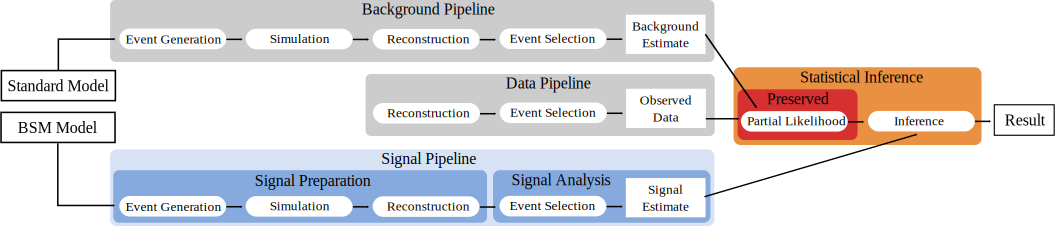
\includegraphics[width=\textwidth]{pipeline}
	\caption{Full analysis workflow including the three main processing pipelines for deriving background and signal estimates as well as observed data rates. The outputs of the three processing pipelines are combined into a likelihood forming the basis for statistical inference. Figure recreated from \reference\cite{ATL-PHYS-PUB-2019-032}.}
	\label{fig:pipeline_analysis}
\end{figure}

\subsection{Necessary ingredients}

As the event selection of an analysis is fixed, the background estimates and observed data in the targeted regions of interest do not change and can be archived in a suitable format. Reinterpreting a search in the light of a new signal model consequently only requires the signal pipeline in~\cref{fig:pipeline_analysis} to be run again, in order to derive the signal estimates that serve as input for the statistical inference. As the data and background processing pipelines shown in~\cref{fig:pipeline_analysis} only enter the statistical inference as estimated event rates, the volume of data that needs to be archived is significantly smaller than the original input data. As will be discussed in~\cref{sec:full_likelihood}, it has recently become technically possible to directly preserve the partial analysis likelihood built from the background estimates and observed data and including all details of the statistical model used for inference. Once the signal estimates are known, a new full analysis likelihood can be built, and the viability of the new signal model can be tested. 

Different approaches exist for deriving signal estimates. Manifestly the most precise approach involves running the original analysis using a different \gls{bsm} model. As this requires to preserve the entirety of the original software and workflows used in the analysis, this is arguably the most involved approach. A framework designed to facilitate such an effort, called \textsc{Recast}, has originally been proposed in \reference\cite{RECAST_cranmer} and aims to provide reintepretations as a service. Through a web interface, physicists would request a reinterpretation of a search, providing an alternative model, triggering a computational workflow executing the original analysis and delivering the recasted results. \Cref{sec:recast_implementation} discusses an attempt at fully preserving the search for electroweakinos presented in this work in the context of \textsc{Recast}. 

In many cases, the full precision of the original analysis pipeline is either not needed, or not accessible. As the full detector simulation requires access to the collaborations's detector description and is the most computationally expensive step in the signal pipeline, even when using fast simulations like \textsc{ATLFAST-II}, it is often approximated using simplified detector geometries and granularities. The most commonly used package for fast detector simulation outside of the collaboration is \textsc{Delphes}~\cite{Delphes:2009tx}. Other packages like \eg \textsc{Rivet}~\cite{Rivet1:2010ar,Rivet2:2019stt} approximate the detector response using dedicated 4-vector smearing techniques, assuming that the detector response roughly factorises into the responses of single particles. Internally, ATLAS also uses a dedicated framework for 4-vector smearing techniques, used in scenarios where other fast simulation techniques are still too expensive. \Cref{sec:truth_smearing} discusses these dedicated smearing functions further.

Similarly to the detector simulation, the analysis-specific event selection is also routinely approximated using different approaches. A number of public tools aiming to reimplement approximations of the event selections of various \gls{bsm} searches are available. Prominent examples include \textsc{CheckMate}~\cite{Checkmate2:2016npn,Checkmate:2013wra} and \textsc{MadAnalysis}~\cite{MadAnalysis:2012fm}. ATLAS has internally maintained a similar catalogue of its \gls{susy} analyses and has published event selection snippets in C++ on \textsc{HEPData}~\cite{HEPData:2017ypu}. Recently, this package maintained by ATLAS, called \textsc{SimpleAnalysis}~\cite{simpleanalysis}, has been made publicly available, allowing the C++ snippets published to be run outside the collaboration.

Instead of trying to estimate the signal rates of a new signal model using \gls{mc} simulation and (reimplemented) analysis event selections, some reinterpretation efforts like \eg \textsc{SModelS}~\cite{SModelS1:2013mwa,SModelS2:2017neo} use \textit{efficiency maps} encoding the selection efficiency of the analysis as a function of some of the analysis observables (typically the sparticle masses). Such efficiency maps are routinely published by the ATLAS \gls{susy} searches on \textsc{HEPData}, and allows for efficient reinterpretations as long as the signal efficiencies mostly depend on the signal kinematics and are largely independent from the specific details of the signal model~\cite{SModelS1:2013mwa}. For the analysis presented in the previous part of this work, the efficiency maps and further analysis data products are available at \reference\cite{HEPdata_1Lbb}. 

\section{Public full likelihood}\label{sec:full_likelihood}

The likelihood is arguably one of the most information-dense and thus valuable data products of an analysis. Without precise knowledge of the exact likelihood of the original analysis, approximations need to be made for the statistical inference \eg in terms of correlations between event rate estimates as well as the treatment of uncertainties. Recently, ATLAS has started to publish full analysis likelihoods built using the \textsc{HistFactory} \gls{pdf} template introduced in~\cref{ch:statistics}~\cite{ATL-PHYS-PUB-2019-029}. This extraordinary step towards more open and reproducible science has been praised by the theory community~\cite{REINP:2020pec} as it allows for considerably more trustful reinterpretations. This effort has been facilitated by the development of \texttt{pyhf} in conjunction with the introduction of a \texttt{JSON} specification fully describing the \textsc{HistFactory} template. As a pure-text format, the \texttt{JSON} likelihoods are human- and machine-readable, highly compressible and can easily be put under version control, all of which are properties that make them ideal for long-term preservation. 

The full likelihood (in \texttt{JSON} format) of the search for electroweakinos presented in the previous part of this work has been published~\cite{fullLH_1Lbb} and is not only heavily used in the following chapters, but also in various analysis reinterpretation and combination efforts currently ongoing in ATLAS. Several efforts outside of the ATLAS collaboration have already included the analysis likelihood into their reinterpretations, \eg \textsc{SModelS}~\cite{SModelS_pyhf:2020grj} and \textsc{MadAnalysis}~\cite{Goodsell:2020ddr,Fuks:2021wpe} both reporting significant precision improvements through the use of the full likelihood (as opposed to approximating the statistical model). Furthermore, the full likelihood of the search presented herein has recently been used to demonstrate the concept of scalable distributed statistical inference on \glspl{hpc}~\cite{Feickert:2021sua}. Through the \texttt{funcX} package~\cite{chard20funcx}, \texttt{pyhf} is used as a highly scalable function as a service to fit the entire signal grid of 125 signal points with a wall time of $\SI{156}{\second}$ using 85 available worker nodes\footnote{Theses benchmarks use \texttt{pyhf}'s \textsc{NumPy} backend and \textsc{SciPy} optimiser, which does have a slower log-likelihood minimisation time than \eg \textsc{PyTorch} coupled with \textsc{SciPy}.}.

\section{Analysis preservation using containerised workflows}\label{sec:recast_implementation}

In order to re-run the original analysis pipeline, the full software environment used for deriving the public analysis results needs to be archived and available. This not only includes the original analysis-specific code used for object definitions, calibrations, event selection and statistical inference, but also the full software necessary for event generation, simulation and reconstruction. Much of the software depends on the  operating system used and a number of low-level system libraries, which also need to be conserved. From a technical point of view, this can be achieved using \textit{Linux containers} 


\textsc{Recast}, originally proposed in \reference\cite{RECAST_cranmer} and recently used within ATLAS in \eg \reference\cite{ATL-PHYS-PUB-2019-032}




 \begin{figure}
	\centering\includegraphics[width=\textwidth]{yadage_workflow_instance}
	\caption{Workflow}
	\label{fig:recast_workflow}
\end{figure}


\cleardoublepage
%!TEX root = ../thesis.tex
%*******************************************************************************
%*********************************** Analysis Overview *********
%*******************************************************************************

\chapter{Simplified likelihoods}\label{ch:simplify}

\ifpdf
    \graphicspath{{chapter-simplify/Figs/Raster/}{chapter-simplify/Figs/PDF/}{chapter-simplify/Figs/}}
\else
    \graphicspath{{chapter-simplify/Figs/Vector/}{chapter-simplify/Figs/}}
\fi

In the previous chapter, the concept of preserving an analysis for the purpose of reinterpretations has been introduced, and an example of a fully preserved analysis pipeline using containerised workflows has been discussed. In large-scale reinterpretations involving a large number of \gls{susy} models to be tested against, the wall time needed for statistical inference can be a computational bottleneck and thus calls for simplifications of the statistical model of an analysis. This chapter therefore introduces the concept of \textit{simplified likelihoods} as approach to approximate the statistical model of an analysis.

\section{Motivation}\label{sec:simplified_likelihood_motivation}

Reinterpretations of ATLAS SUSY searches in more complete and realistic \gls{susy} scenarios (as opposed to simplified models) often involves high-dimensional parameter spaces that are computationally extremely challenging to sample and compare to ATLAS data in an exhaustive way. Large-scale reinterpretations of this type have already been performed in ATLAS after the Run~1 data-taking period in both the 19-dimensional \gls{pmssm}~\cite{SUSY-2014-08} (introduced in~\cref{sec:theory_pmssm}) as well as a 5-dimensional representation of the \gls{pmssm}~\cite{Aaboud:2016wna}. Due to the complexity of the statistical models of today's SUSY searches in ATLAS, originating from the large number of channels and the large amount of nuisance parameters typically considered, the wall time needed for the statistical inference is usually far from negligible. In a typical large-scale reinterpretation involving $\mathcal{O}(10^5-10^6)$ sampled models, an optimistic estimation of the wall time needed for the statistical inference per model of $\mathcal{O}(\SI{10}{\second}-\SI{e2}{\second})$ is too computationally expensive, especially when more than just a few ATLAS \gls{susy} searches are included.

One approach of alleviating this computational problem is to approximate the \gls{susy} searches through their model-independent limits published in conjunction with the model-dependent exclusion limits. By construction, the model-independent limits are derived using only cut-and-count signal regions without multi-bin or shape-fit setups, thus making minimal model assumptions. While computationally very fast, this approach naturally underestimates the true exclusion power of the respective analysis due to the fact that model-dependent properties are not exploited (as they typically are in the exclusion signal regions). \Cref{fig:single_bin} compares the exclusion contours obtained with the full set of exclusion signal regions (shown in orange) to the exclusion contours obtained using the discovery signal regions (shown in green), defined in~\cref{tab:SignalRegionDef}. As the discovery signal regions are not mutually exclusive, they are not statistically combined and thus three separate observed and expected contours can be drawn. From \cref{fig:single_bin}, it is clear that even a best-expected combination of the three discovery signal regions does not reach the sensitivity achieved using the two-dimensional shape-fit setup resulting from statistical combination of the nine exclusion signal regions. Nonetheless, this approach has been opted for in the large-scale scan of the \gls{pmssm} using ATLAS data from Run~1~\cite{SUSY-2014-08}, yielding conservative exclusion power and thus room for improvement.

Therefore, the following sections introduce a method for approximating ATLAS SUSY searches without disregarding their elaborate use of multi-bin signal regions exploiting the varying shapes of signal and \gls{sm} background distributions. 

\begin{figure}
	\centering
	\begin{subfigure}[b]{0.5\textwidth}
		\centering\includegraphics[width=\textwidth]{exclusion_1Lbb_SRLM_noLabel}
		\caption{Discovery SR-LM\label{fig:single_bin_SRLM}}
	\end{subfigure}\hfill
	\begin{subfigure}[b]{0.5\textwidth}
		\centering\includegraphics[width=\textwidth]{exclusion_1Lbb_SRMM_noLabel}
		\caption{Discovery SR-MM\label{fig:single_bin_SRMM}}
	\end{subfigure}\hfill
	\begin{subfigure}[b]{0.5\textwidth}
		\centering\includegraphics[width=\textwidth]{exclusion_1Lbb_SRHM_noLabel}
		\caption{Discovery SR-HM\label{fig:single_bin_SRHM}}
	\end{subfigure}%
	\caption{Comparison of exclusion limits obtained using a likelihood built from all nine exclusion signal regions (orange), and the discovery signal regions (green). As discussed in~\cref{sec:signal_region_definitions}, the discovery signal regions are simple cut-and-count regions with minimal model assumptions. They are not mutually exclusive, they cannot be fitted together, thus resulting in three separate exclusion contours. All statistical and systematic uncertainties on the background and the signal event rates are included.}\label{fig:single_bin}
\end{figure}

\section{Building simplified likelihoods}\label{sec:building_simplified_likelihoods}



In order to retain the full statistical combination of multiple signal region bins implemented in many SUSY searches, while still being able to achieve a sufficiently fast approximation, the statistical treatment of the systematic uncertainties as well as of the background model needs to be simplified. In the procedure presented in the following, this is achieved by first performing a background-only fit to data in all \glspl{sr} and \glspl{cr}, in order to determine the best-fit values of all the model parameters $\boldsymbol{\phi}$. This allows to calculate the post-fit total background estimate as well as the total uncertainty on the estimate in every bin, both of which can be used to construct a simplified likelihood.

As the full likelihood in \texttt{JSON} format defines the full statistical model used for the statistical inference, the above background-only fit can be performed using \texttt{pyhf} and the preserved full likelihood of the analysis. With the full likelihoods starting to become available on \textsc{HEPData} (see \eg \reference\cite{fullLH_1Lbb}) this procedure can rely on public information only and is therefore widely accessible to the \gls{hep} community. The simplified likelihoods introduced in the following, follow the same \texttt{JSON} specification introduced for the full likelihoods in \reference\cite{ATL-PHYS-PUB-2019-029}. The following description highlights the specification details relevant to the simplified likelihood. 

\subsubsection{Background model}

In the simplified likelihood, the background model is approximated with a single background sample, representing the total \gls{sm} background estimate in the different analysis channels (called \texttt{total\_bkg} in \cref{lst:bkg_sample}). The sample rate of the total background sample is set to the total post-fit background estimate obtained in the background-only fit using the full statistical model (in \cref{lst:bkg_sample} set to be $10.0$). Likewise, the complete set of nuisance parameters in the original full likelihood is reduced to a single constrained parameter $\alpha$ with up and down variations corresponding to the post-fit uncertainties on the total \gls{sm} background estimates in each bin (called \texttt{total\_error} in \cref{lst:bkg_sample}). It is constrained by a Gaussian $\mathrm{Gaus}(a = 0 \vert \alpha , \sigma = 1)$ and is correlated over all bins in each channel. Although the final uncertainty is constrained by a simple Gaussian, the full treatment of the uncertainties in the background-only fit using the full likelihood ensures that non-Gaussian effects are included to some extent.

\begin{minipage}{\linewidth}
\begin{lstlisting}[language=json,firstnumber=1,caption={Example of a total background sample with sample rate and total uncertainty as derived from a previous fit in the \glspl{sr} and \glspl{cr}.},captionpos=b, label=lst:bkg_sample]
{
	"name": "total_bkg",
	"data": [10.0],
	"modifiers": [{"data": {"hi_data": [12.0], "lo_data": [8.0]}, "name": "total_error", "type": "histosys"}]
}
\end{lstlisting}
\end{minipage}

\subsubsection{Analysis channels}

Each original channel in the full likelihood with the original number of bins is also entering the simplified likelihood, and each contains the total background sample as specified above. Apart from the total background sample, one additional sample is needed---the signal sample. An example of a signal sample is shown in \cref{lst:sig_sample}. It introduces the unconstrained signal strength parameter $\mu$ as second parameter of the statistical model. For simplicity, the example shown in \cref{lst:sig_sample} does not introduce any additional uncertainties on the signal rates, thereby assuming that them to be negligible. Depending on the \gls{bsm} scenario, signal uncertainties can be introduced through additional nuisance parameters (modifiers).

\begin{minipage}{\linewidth}
\begin{lstlisting}[language=json,firstnumber=1,caption={Example of a signal sample with sample rate and unconstrained normalisation parameter.},captionpos=b, label=lst:sig_sample]
{
	"name": "signal",
	"data": [7.0],
	"modifiers": [{"data": null, "name": "mu_Sig", "type": "normfactor"}]
}
\end{lstlisting}
\end{minipage}

\subsubsection{Observations and measurements}

According to the \texttt{JSON} specification defined in \reference\cite{ATL-PHYS-PUB-2019-029}, the data observed by the analysis in each channel (and each bin) is introduced by means of an \textit{observation}. In the case of the simplified likelihood, this is taken directly from the full likelihood and, by construction, does not need to be modified. An example of an observation including several channels and bins is shown in~\cref{lst:observation}.

\begin{minipage}{\linewidth}
\begin{lstlisting}[language=json,firstnumber=1,caption={Example of an observation in the simplified likelihood. It can be directly taken from the corresponding full likelihood. This example implements three channels, two with one bin, and one with three bins.},captionpos=b, label=lst:observation]
{
	"observations": {
		{"name": "channel_A" : "data": [25.0]},
		{"name": "channel_B" : "data": [20.0]},
		{"name": "channel_C" : "data": [11.0, 13.0]}
	}	
}
\end{lstlisting}
\end{minipage}

The only part of the \texttt{JSON} specification left to be defined is the \textit{measurement}, specifying the name of the parameter of interest as well as parameter set configurations not already covered in the channel definitions. For the simplified likelihood, it is straightforward to write down, as can be seen in~\cref{lst:measurement}.

\begin{minipage}{\linewidth}
\begin{lstlisting}[language=json,firstnumber=1,caption={Example of a measurement in the simplified likelihood. The signal strength is the parameter of interest, no additional parameters need further configuration.},captionpos=b, label=lst:measurement]
{
	"measurements": {
		"name": "myMeasurement",
		"config": { "poi": "mu_Sig", "parameters": []}
	}	
}
\end{lstlisting}
\end{minipage}

Put together, the above pieces result in a simplified likelihood for a given signal model, using a background model obtained from an initial background-only fit using the full likelihood considering the full treatment of systematic uncertainties. Replacing the signal sample by the means of \texttt{JSON} patches allows for systematic reinterpretations of any signal model for which the expected rates in the analysis regions are known.  


\section{Computational performance}\label{sec:cpu_performance}

One of the main figures of merit of an analysis approximation naturally is the reduction in wall time compared to the full analysis. \Cref{fig:benchmark_1Lbb} shows a benchmark for different likelihood configurations of the search for electroweakinos presented herein. The wall time of the full analysis likelihood is compared with that of the simplified likelihood constructed following the previously introduced prescription. In addition, the wall time of the single-bin likelihood using the discovery \glspl{sr} in a setup similar to that already used in the naive approximation in \cref{fig:single_bin}, is shown. For each likelihood, different computational backends are used for the tensor algebra operations in \texttt{pyhf}. All benchmarks have been performed on an Intel i7-4790 CPU with a nominal clock speed of $\SI{3.60}{\GHz}$, 4 cores and 8 threads. The CPU was not isolated but under minimal load. The original 125 signal points of the analysis where used in each configuration.

\begin{figure}
	\centering    
	\includegraphics[width=\textwidth]{benchmark_1Lbb}
	\caption{Benchmarks of the CPU-time necessary for hypothesis testing using different likelihood and \texttt{pyhf} configurations in the context of the ATLAS 1L electroweakino search, run on a non-isolated CPU with 4 threads. The full likelihood (left) includes the full statistical implementation of the original analysis, the simplified likelihood (center) represents the simplified likelihood approach presented in this document, and the single-bin likelihood (right) represents a single-bin approximation of the ATLAS 1L electroweakino search. The uncertainties represent the standard deviation of the benchmark test sample.}\label{fig:benchmark}
	\label{fig:benchmark_1Lbb}
\end{figure}

The use of automatic differentiation of the full likelihood gradient enabled by some of the tensor algebra backends to \texttt{pyhf} offers an efficient minimisation of the likelihood resulting in fast hypothesis tests of $\mathcal{O}(\SI{5}{\second})$ for the full analysis. In large-scale reinterpretations, this is however still to computationally expensive. The simplified likelihood, on the other hand, results in a wall time for hypothesis tests as fast as $\SI{0.04}{\second}$ per signal model. Thus, the computational performance of the simplified likelihood is in the same order of magnitude as that of the naive single-bin approach\footnote{In fact, the simplified likelihood is actually even faster than the single-bin approach, as the latter needs to be executed separately for each discovery \gls{sr} and thus the numbers quoted need to be multiplied by the number of discovery \glspl{sr} used in the analysis.}, but offers by construction a significantly better approximation oft the true analysis exclusion power.

Interestingly, the wall time of the simplified likelihood does not benefit from the usage of features like automatic differentiation offered by \eg \textsc{PyTorch}. This is due to the extreme simplicity of the simplified likelihood function, therefore the computational benefits from features like automatic differentiation do not outweigh the overhead of libraries like \textsc{PyTorch}.

In addition to the search for electroweakinos presented herein, the simplified likelihood approach has also been applied on a number of other ATLAS SUSY searches. \Cref{tab:simplified_performance} 

\begin{table}
	\begin{center}
	\small
			\begin{tabular} {l r r}
				\toprule
				Analysis & Full likelihood [s] & Simplified likelihood [s] \\
				\midrule
				ATLAS compressed search~\cite{SUSY-2018-16} & 0 & 0 \\
				ATLAS 3-lepton search & 0 & 0 \\
				ATLAS 2-lepton search~\cite{SUSY-2018-32} & 0 & 0 \\
				ATLAS 1-lepton search~\cite{SUSY-2019-08} & 0 & 0 \\
				ATLAS direct stau search~\cite{SUSY-2018-04} & 0 & 0 \\
				ATLAS sbottom search~\cite{SUSY-2018-31} & 0 & 0 \\
				ATLAS stop search & 0 & 0 \\
				\bottomrule
			\end{tabular}
		\caption{}
		\label{tab:simplified_performance}
	\end{center}
\end{table}

\section{Physics performance}\label{sec:physics_performance}

A comparison of the exclusion contours obtained with the full and simplified likelihoods in the context of the search for electroweakinos presented herein is shown in~\cref{fig:results_simplify_1Lbb}. The results obtained using the simplified likelihood are shown in blue, while the results obtained using the full likelihood are presented in orange. Both the observed (without the usual theoretical up and down variations on the signal cross section) and expected exclusion limits including the uncertainty band are shown. In the case of the full likelihood, the complete set of \gls{mc} statistical and systematic uncertainties introduced in \cref{ch:uncertainties} are taken into account. As discussed in \cref{sec:building_simplified_likelihoods}, the uncertainty band on the simplified likelihood contour results from the single nuisance parameter built by reducing the original nuisance parameters.

The exact observed and expected CL$_s$ values obtained using both likelihoods are shown in~\cref{fig:scatter_cls}. As expected from the exclusion contour, both the simplified and the full likelihood agree reasonably well across the majority of the shown range in CL$_s$. For signal models highly excluded with the full likelihood, \ie $\mathrm{CL}_s \ll 0.05$, the simplified likelihood tends to result in slightly larger CL$_s$ values than the full likelihood, thus giving a conservative sensitivity estimate. In the range relevant to the exclusion contour at 95\% CL, the results from the simplified likelihood agree well with those from the full likelihood.

\begin{figure}
\floatbox[{\capbeside\thisfloatsetup{capbesideposition={right,center},capbesidewidth=0.35\textwidth}}]{figure}[\FBwidth]
{\caption{Comparison of the simplified likelihood (blue contours) and full likelihood (orange contours) results for the search for electroweakinos presented previously. The observed contours are shown as solid lines, while the expected contours are shown as dashed lines. The uncertainty band includes all \gls{mc} statistical and systematic uncertainties in the case of the full likelihood, and only the simplified uncertainties in the case of the simplified likelihood.}\label{fig:results_simplify_1Lbb}}
{\includegraphics[width=0.60\textwidth]{exclusion_1Lbb_noLabel}}
\end{figure}

\begin{figure}
	\centering
	\begin{subfigure}[b]{0.5\textwidth}
		\centering\includegraphics[width=\textwidth]{cls_scatter_lin}
		\caption{Linear scale}
	\end{subfigure}\hfill
	\begin{subfigure}[b]{0.5\textwidth}
		\centering\includegraphics[width=\textwidth]{cls_scatter_log}
		\caption{Logarithmic scale}
	\end{subfigure}
	\caption{Scatter plots comparing the observed and expected CL$_s$ values obtained using the simplified and the full likelihoods for the same set of signal models considered in the search for electroweakinos. Both linear and logarithmic scale representations are shown.}\label{fig:scatter_cls}
\end{figure}


In addition to the search for electroweakinos presented herein, the simplified likelihood approach has been applied on a number of additional ATLAS SUSY searches. An overview of the results can be seen in~\cref{fig:results_analyses}



\begin{figure}
	\centering
	\begin{subfigure}[b]{0.5\textwidth}
		\centering\includegraphics[width=\textwidth]{exclusion_sbottom_noLabel}
		\caption{ATLAS sbottom search~\cite{SUSY-2018-31}\label{fig:results_sbottom}}
	\end{subfigure}\hfill
	\begin{subfigure}[b]{0.5\textwidth}
		\centering\includegraphics[width=\textwidth]{exclusion_stop1L_noLabel}
		\caption{ATLAS stop search\label{fig:results_stop1L}}
	\end{subfigure}\hfill
	\begin{subfigure}[b]{0.5\textwidth}
		\centering\includegraphics[width=\textwidth]{exclusion_2L0J_noLabel}
		\caption{ATLAS 1L search~\cite{SUSY-2019-08}\label{fig:results_2L0J}}
	\end{subfigure}\hfill
	\begin{subfigure}[b]{0.5\textwidth}
		\centering\includegraphics[width=\textwidth]{exclusion_directstaus_noLabel}
		\caption{\label{fig:results_directstaus}}
	\end{subfigure}\hfill
	\begin{subfigure}[b]{0.5\textwidth}
		\centering\includegraphics[width=\textwidth]{exclusion_3Loffshell_noLabel}
		\caption{ATLAS 2L search~\cite{SUSY-2018-32}\label{fig:results_3Loffshell}}
	\end{subfigure}\hfill
	\begin{subfigure}[b]{0.5\textwidth}
		\centering\includegraphics[width=\textwidth]{exclusion_compressed_noLabel}
		\caption{ATLAS compressed electroweakino search~\cite{SUSY-2018-16}\label{fig:results_compressed}}
	\end{subfigure}\hfill
	\caption{Simplified likelihood results for the different ATLAS searches studied in this document. The results from the simplified likelihood (blue) are compared with the results of the full analysis likelihood (orange). The coloured numbers represent the observed CL$_s$ numbers obtained with both likelihoods.}\label{fig:results_analyses}
\end{figure}


\section{Limitations and future prospects}

\cleardoublepage
%!TEX root = ../thesis.tex
%*******************************************************************************
%*********************************** Analysis Overview *********
%*******************************************************************************

\chapter{Reinterpretation in the pMSSM}\label{ch:pmssm}

\ifpdf
    \graphicspath{{chapter-pmssm/Figs/Raster/}{chapter-pmssm/Figs/PDF/}{chapter-pmssm/Figs/}}
\else
    \graphicspath{{chapter-pmssm/Figs/Vector/}{chapter-pmssm/Figs/}}
\fi

After having discussed to some extent efforts and methods to reinterpret ATLAS searches for \gls{susy}, this chapter presents a reinterpretation of the 1-lepton analysis in the \gls{pmssm}. The truth analysis and simplified likelihoods discussed in~\cref{ch:preservation,ch:simplify}, respectively, are instrumental for the following sections. 

\section{Motivation}

In today's searches for \gls{bsm} physics, it is common to use simplified models as a way of avoiding to necessity to deal with high-dimensional parameter spaces that are extremely challenging to sample and compare to data in an exhaustive way. The simplified model approach has also been used in the second part of this work, where results of the interpretation of the 1-lepton analysis in the $\charg\neutr\rightarrow Wh\lsp\lsp$ model have been presented. As has been discussed in~\cref{sec:simplified_models}, simplified models are however by no means complete \gls{susy} models and only serve as proxies for more complex and realistic \gls{susy} scenarios. As such, simplified model limits cannot trivially be translated into limits on model parameters of a more complete \gls{susy} model. Large-scale reinterpretations are necessary to understand the constraints today's \gls{susy} searches set on realistic \gls{susy} scenarios. 

One class of more complete models, focussing on phenomenologically viable models, is the \gls{pmssm}, introduced in~\cref{sec:theory_pmssm}. With its 19 parameters it offers much more complex \gls{susy} scenarios while still being of somewhat manageable dimensionality. Still, large-scale reinterpretations in the \gls{pmssm} are computationally challenging and require a set of approximation as those introduced in~\cref{ch:preservation,ch:simplify}.

Large-scale reinterpretations in the \gls{pmssm} using a collection of relevant ATLAS \gls{susy} searches not only allow to assess the sensitivity of the ATLAS \gls{susy} search program towards more realistic \gls{susy} scenarios, but can also potentially reveal interesting regions of the parameter space not yet covered by the current search programme. Moreover, such reinterpretations allow to demonstrate the sensitivity of simplified model searches beyond the simplified models they are originally interpreted in, thereby justifying the use of simplified models as proxies for more complete \gls{susy} scenarios. In addition, reinterpretations in the \gls{pmssm} can be used to connect the ATLAS \gls{susy} searches with dark matter constraints from non-collider experiments, as well as Higgs and flavour measurements. \unsure{might want to tweak this last sentence} 

Although the following sections will be restricted to a reinterpretation of the 1-lepton search presented in the second part of this thesis, efforts are ongoing in ATLAS to perform large-scale reinterpretations using a majority of the full Run~2 ATLAS \gls{susy} searches. These efforts will most likely result in one of the most comprehensive set of ATLAS constraints on \gls{susy} yetope.

\section{Truth-level analysis}\label{sec:truth_analysis}

As discussed in~\cref{ch:preservation}, the reinterpretation of an analysis involves re-executing the analysis pipeline in order to derived signal rate estimates in all regions. In large-scale reinterpretations, running a \textsc{Recast} implementation on all signal models considered is not computationally feasible and instead a \textit{truth-level} analysis is first performed for all signal models sampled. Only models with uncertain exclusion at truth-level are processed through the computationally expensive full analysis chain implemented in \textsc{Recast}. The truth-level analysis skips the detector simulation and uses generator-level objects instead. Any detector-level effects and inefficiencies will thus not be reflected in truth-level observables. In order to reproduce the kinematic distributions observed in the full analysis (using reconstruction-level objects), a dedicated \textit{truth smearing}---discussed in detail in~\cref{sec:truth_smearing}---is applied.

\subsection{Truth selection}\label{sec:truth_selection}

 \begin{figure}
	\centering
	\begin{subfigure}[b]{0.45\linewidth}
		\centering\includegraphics[width=\textwidth]{20210324_noLabel_noOR/700_150/lep1Pt_C1N2_Wh_hbb_700p0_150p0_smeared.pdf}
	\end{subfigure}\hfill
	\begin{subfigure}[b]{0.45\linewidth}
		\centering\includegraphics[width=\textwidth]{20210324_noLabel_noOR/700_150/jet1Pt_C1N2_Wh_hbb_700p0_150p0_smeared.pdf}
	\end{subfigure}\hfill
	\caption{Impact of the overlap removal procedure at truth-level illustrated in the lepton and leading jet transverse momenta distributions. The truth-distribution without overlap removal (green) generally underestimates the number of signal events at reconstruction-level (orange). Correct overlap removal procedure at truth-level (blue) improves the agreement. The exemplary benchmark signal point with $m(\charg/\neutr), m(\lsp) = 700, \SI{150}{\GeV}$ is shown in both plots (at truth- and reconstruction-level). All distributions are shown in a loose preselection requiring exactly one lepton, $\met>\SI{50}{\GeV}$, $\mt > \SI{50}{\GeV}$, and 2--3 jets, two of which need to be \textit{b}-tagged.}
	\label{fig:overlap_removal_truth}
\end{figure}

All signal and control regions considered in the original 1-lepton search are implemented at truth-level using \textsc{SimpleAnalysis}. The exact implementation is publicly available at \reference\cite{HEPdata_1Lbb} and was already used in~\cref{ch:uncertainties} for the derivation of some of the theory uncertainties in the full analysis.

The truth-level implementation full specifies all object definitions introduced in~\cref{sec:object_definitions} even though some of them, like \eg lepton isolation, are technically not well-defined at truth-level The subsequent smearing is in many cases implemented as a function of said object definitions and thus allows to consider them nonetheless. Additionally, as discussed in~\cref{sec:reinterpretations}, the full specification of the original analysis event selection including all object definitions allows for simpler reinterpretations by efforts outside of the ATLAS collaboration that generally do not have access to the original analysis software.

Following the object definitions, an overlap removal procedure following the same prescription as described for the reconstruction-level analysis is performed, \ie especially also using the same shrinking cone definitions introduced in~\cref{sec:overlap_removal}. Overlap removal step removing electrons sharing a track with a muon is approximated by using a distance parameter of $\Delta R = 0.01$ between the objects. Although often neglected\footnote{The overlap removal procedures in ATLAS \gls{susy} searches tend to be quite intricate, making them non-trivial to re-implement without ATLAS and analysis-specific knowledge.} in reinterpretation efforts outside of the collaboration, the correct implementation of the overlap removal procedure employed in the original analysis is typically crucial to reproduce the signal estimates of the original analysis, as illustrated in~\cref{fig:overlap_removal_truth}. Furthermore, the exact implementation of all analysis observables is explicitly given in the \textsc{SimpleAnalysis} implementation, followed by the full definition of all control and signal regions.

\subsection{Truth smearing}\label{sec:truth_smearing}

The general assumption of the truth smearing applied in the following is that the detector response roughly factorises into the responses of single particles. This allows to use detector performance results provided by ATLAS in order to construct detector response maps parameterised in different observables for each physics object. Detector response maps include object reconstruction and identification efficiencies as well as scale factors to correct for differences between \gls{mc} and observed data. Likewise, effects from the finite resolution of energy measurements in the detector are modelled through energy resolution maps. In the following, the 4-vector components of electrons, muons, jets and $\etmiss$ are smeared. The implementation of the smearing functions is internal to ATLAS and originates predominantly from various upgrade studies.

In the case of truth electrons, the identifications efficiencies considered are parameterised in $\eta$ and $\pt$ as well as the identification working point used. In $\eta$, nine fixed-width bins are used. In $\pt$, six bins are implemented and a linear interpolation between two adjacent $\pt$-bins is used to get the efficiency for the given $\pt$ of each truth electron. The probability of finding a fake electron in a truth jet is estimated through a similar two-dimensional map depending on the truth jet $\eta$ and $\pt$, again using fixed-width bins in $\eta$ and a linear interpolation in $\pt$. The range of the $\pt$ interpolation for identification efficiencies and fake rates extends from $\SI{7}{\GeV}$ to $\SI{120}{\GeV}$. If the truth $\pt$ of the electron is outside of that range, the identification efficiency and fake rate from the respective bound of the corresponding $\eta$-bin are used. The probability for misidentifying an electron as a photon is estimated using different fixed values for the barrel and end-cap regions. Finally, the transverse energy of the electron is smeared using a random number drawn from a Gaussian distribution with  standard deviation corresponding to the $\eta$- and $\pt$-dependent energy resolution.  

For truth muons, the identification efficiencies are also parameterised in $\eta$ and $\pt$ as well as the identification working point used. Similar to truth electrons, the  $\pt$ of the muon is smeared using a Gaussian distribution with standard deviation corresponding to the momentum resolution. The momentum resolution of combined truth muons, $\sigma_\mathrm{CB}$, is computed from the measured resolutions in the \gls{id},$\sigma_\mathrm{ID}$, and \gls{ms}, $\sigma_\mathrm{MS}$, as
\begin{equation}
	\sigma_\mathrm{CB} = \frac{\sigma_\mathrm{ID}\sigma_\mathrm{MS}}{\sqrt{\sigma_\mathrm{ID}^2 + \sigma_\mathrm{MS}^2}},
\end{equation}
where $\sigma_\mathrm{ID}$ and $\sigma_\mathrm{MS}$ are parameterised in $\eta$ and $\pt$.

The transverse momentum of truth jets is smeared using a Gaussian with standard deviation equal to the \gls{jer}, provided in a map parameterised in five bins in $\eta$ ranging from $\vert\eta\vert = 0$ to $\vert\eta\vert = 4.5$. Following~\cite{Aad:2020flx}, jet energy resolutions are provided using parameterisations of a noise $N$, stochastic $S$ and constant $C$ term for each of the seven bins in $\vert\eta\vert$, such that the resolution can be computed as
\begin{equation}
	\frac{\sigma(\pt)}{\pt} = \frac{N}{\pt}\oplus\frac{S}{\sqrt{\pt}}\oplus C.
\end{equation}
Only truth jets with $\SI{10}{\GeV} < \pt < \SI{1.5}{\TeV}$ are smeared. For truth jets with $\pt > \SI{20}{\GeV}$, the flavour tagging efficiency is considered using efficiencies parameterised in $\eta$, $\pt$ and the \textsc{MV2c10} working point (introduced in~\cref{sec:object_definitions}) used, measured in fully reconstructed simulated $\ttbar$ events~\cite{FTAG-2018-01}.

Finally, the smeared missing transverse energy is computed using the transverse momenta of all smeared truth objects in the event, including an approximation for the track soft term. The latter is approximated using results from $Z\rightarrow e^+e^-$ events, allowing to infer a distribution of the mean soft term projected in the direction longitudinal to the total transverse momentum of all hard objects in an event, $\boldsymbol{p}_\mathrm{T}^\mathrm{hard}$. The measured resolution parallel and perpendicular to $\boldsymbol{p}_\mathrm{T}^\mathrm{hard}$ is then used to smear the nominal soft track value.
 
  \begin{figure}
	\centering
	\begin{subfigure}[b]{0.45\linewidth}
		\centering\includegraphics[width=\textwidth]{20210324/700_150/met_C1N2_Wh_hbb_700p0_150p0_smeared.pdf}
	\end{subfigure}\hfill
	\begin{subfigure}[b]{0.45\linewidth}
		\centering\includegraphics[width=\textwidth]{20210324/700_150/mt_C1N2_Wh_hbb_700p0_150p0_smeared.pdf}
	\end{subfigure}\hfill
	\begin{subfigure}[b]{0.45\linewidth}
		\centering\includegraphics[width=\textwidth]{20210324/700_150/mct_C1N2_Wh_hbb_700p0_150p0_smeared.pdf}
	\end{subfigure}\hfill
	\begin{subfigure}[b]{0.45\linewidth}
		\centering\includegraphics[width=\textwidth]{20210324/700_150/mbb_C1N2_Wh_hbb_700p0_150p0_smeared.pdf}
	\end{subfigure}\hfill
	\begin{subfigure}[b]{0.45\linewidth}
		\centering\includegraphics[width=\textwidth]{20210324/700_150/lep1Pt_C1N2_Wh_hbb_700p0_150p0_smeared.pdf}
	\end{subfigure}\hfill
	\begin{subfigure}[b]{0.45\linewidth}
		\centering\includegraphics[width=\textwidth]{20210324/700_150/jet1Pt_C1N2_Wh_hbb_700p0_150p0_smeared.pdf}
	\end{subfigure}\hfill
	\begin{subfigure}[b]{0.45\linewidth}
		\centering\includegraphics[width=\textwidth]{20210324/700_150/mlb1_C1N2_Wh_hbb_700p0_150p0_smeared.pdf}
	\end{subfigure}\hfill
	\begin{subfigure}[b]{0.45\linewidth}
		\centering\includegraphics[width=\textwidth]{20210324/700_150/nBJet30_C1N2_Wh_hbb_700p0_150p0_smeared.pdf}
	\end{subfigure}\hfill
	\caption{Comparisons of the kinematic distributions of key observables at (smeared) truth- and reconstruction-level. The exemplary benchmark signal point with $m(\charg/\neutr), m(\lsp) = 700, \SI{150}{\GeV}$ is shown. The ratio pad shows the ratio between smeared and unsmeared truth-level distributions (blue and green) to reconstruction-level distributions (orange). Only \gls{mc} statistical uncertainty is included in the error bars. All distributions are shown in a loose preselection requiring exactly one lepton, $\met>\SI{50}{\GeV}$, $\mt > \SI{50}{\GeV}$, and 2--3 jets, two of which need to be \textit{b}-tagged. The latter requirement is dropped for the \textit{b}-jet multiplicity distribution.}
	\label{fig:smearing_preselection}
\end{figure}
 
\section{Validation of the truth-level analysis}

\subsection{Validation in loose preselection}

 The performance of the truth smearing is illustrated in a loose preselection for a single exemplary benchmark signal point in~\cref{fig:smearing_preselection}. The loose preselection applied requires exactly one lepton, $\met>\SI{50}{\GeV}$, $\mt > \SI{50}{\GeV}$, and 2--3 jets, two of which need to be \textit{b}-tagged. The reconstruction-level distributions are compared with the truth-level distributions before and after truth smearing. It can clearly be observed that the truth smearing noticeably improves the agreement between the truth- and reconstruction-level distributions. While the lepton and jet reconstruction and identification efficiencies are---due to their dependence on $\eta$, $\pt$ and individual working points---crucial for the overall agreement in shape, the inclusion of flavour-tagging efficiencies significantly improves the overall agreement in normalisation.
 
Although some minor differences remain, overall a good agreement is observed across all relevant kinematic distributions at loose preselection level. Most of the differences between smeared truth-level and reconstruction-level distributions in individual bins are well within the \gls{mc} statistical uncertainties arising from the relatively limited \gls{mc} statistics available.
 
 \subsection{Validation in signal regions}

 \begin{figure}
	\centering
	\begin{subfigure}[b]{0.49\linewidth}
		\centering\includegraphics[width=\textwidth]{yields_SR-LM_unsmeared}
	\end{subfigure}\hfill
	\begin{subfigure}[b]{0.49\linewidth}
		\centering\includegraphics[width=\textwidth]{yields_SR-LM_smeared}
	\end{subfigure}\hfill
	\begin{subfigure}[b]{0.49\linewidth}
		\centering\includegraphics[width=\textwidth]{yields_SR-MM_unsmeared}
	\end{subfigure}\hfill
	\begin{subfigure}[b]{0.49\linewidth}
		\centering\includegraphics[width=\textwidth]{yields_SR-MM_smeared}
	\end{subfigure}\hfill
	\begin{subfigure}[b]{0.49\linewidth}
		\centering\includegraphics[width=\textwidth]{yields_SR-HM_unsmeared}
	\end{subfigure}\hfill
	\begin{subfigure}[b]{0.49\linewidth}
		\centering\includegraphics[width=\textwidth]{yields_SR-HM_smeared}
	\end{subfigure}
	\caption{Comparison of the event rates at truth- and reconstruction-level before (left) and after (right) truth smearing. From top to bottom, the SR-LM, SR-MM and SR-HM signal regions are shown, with cumulative (integrated) $\mct$ bins. Every single point in the scatter plots represents a single signal model considered in the original 1-lepton analysis. Uncertainties include \gls{mc} statistical uncertainties.}
	\label{fig:smearing_signal_regions}
\end{figure}
 
 As the expected signal rates in the signal regions are ultimately what is entering the (simplified) likelihood, it is important that the good agreement observed at preselection is still present in the kinematically tighter selections of the signal regions. Additionally, it is worth investigating the agreement across all signal models considered in the original analysis, as opposed to only validating specific benchmark points. A comparison of the reconstruction-level and truth-level event rates before and after smearing in the signal regions SR-LM, SR-MM and SR-HM is shown in~\cref{fig:smearing_signal_regions} for all signal models considered in the 1-lepton analysis. For the sake of conciseness, only the cumulative $\mct$ bins are shown in each \gls{sr} in~\cref{fig:smearing_signal_regions}. The agreement in the individual $\mct$ bins in each SR-LM, SR-MM and SR-HM is provided in~\cref{fig:smearing_signal_regions_1,fig:smearing_signal_regions_2,fig:smearing_signal_regions_3}.
 
The truth smearing drastically improves the agreement in event rate estimates at truth- and reconstruction-level across all \gls{sr} bins considered. While the event rates are generally overestimated at truth-level before smearing, compared to reconstruction-level, both tend to agree well within statistical uncertainties after smearing. 
 
\subsection{Validation using likelihood}


 \begin{figure}
	\centering
	\begin{subfigure}[b]{0.49\linewidth}
		\centering\includegraphics[width=\textwidth]{exclusion_1Lbb_truthInput_compareReco_BkgOnly_noLabel}
		\caption{\label{fig:full_truth_result}}
	\end{subfigure}\hfill
	\begin{subfigure}[b]{0.49\linewidth}
		\centering\includegraphics[width=\textwidth]{exclusion_1Lbb_truthInput_BkgSignal_700_200_noLabel}
		\caption{\label{fig:simplified_truth_result}}
	\end{subfigure}\hfill
	\caption{Expected and observed exclusion contours obtained with the full and simplified likelihoods. Fig.~\subref{fig:full_truth_result} compares the full likelihood contours obtained with the reconstruction-level inputs (orange) to results obtained with truth inputs before (purple) and after (green) smearing. Fig.~\subref{fig:simplified_truth_result} compares the full likelihood reconstruction-level contours (orange) with those obtained using the simplified likelihood and smeared truth-level inputs (blue). Uncertainties include all statistical and systematic uncertainties on the background and signal for the reconstruction-level contours, but only statistical and systematic uncertainties on the background for truth-level signal inputs.}
	\label{fig:smearing_signal_regions}
\end{figure}

Using the nominal expected event rates at smeared truth-level for every signal model in the original signal grid considered in the 1-lepton analysis, expected and observed CL$_s$ values can be computed and exclusion contours can be derived. \Cref{fig:full_truth_result} compares the expected and observed exclusion contours obtained using the full likelihood and reconstruction-level signal inputs with those obtained using the full likelihood and truth-level signal inputs before and after truth smearing. While all theory and systematic uncertainties on the signal are included in the reconstruction-level contours, no signal uncertainties are considered when obtaining both the smeared and unsmeared truth-level contours. As expected from the previous validation steps in the signal regions, the sensitivity using unsmeared truth-level signal inputs is significantly overestimated compared to the published analysis exclusion limit using reconstruction-level inputs. The smeared truth-level inputs, however, yield exclusion contours with an acceptable match compared to the reconstruction-level results.

With the truth smearing validated at multiple selection levels of the analysis, the full two-fold approximation of signal pipeline and statistical inference can be constructed. \Cref{fig:simplified_truth_result} compares the exclusion contours of the original analysis results with those obtained using smeared truth-level signal inputs as well as the simplified likelihood. Even with the approximations made, overall a good agreement is found and the original analysis results can be reproduced to a relatively high degree of precision.

In summary, this validation process shows that the signal pipeline in~\cref{fig:pipeline_analysis} can be efficiently approximated using truth-level analysis and a simplified treatment of the statistical model, allowing a considerably faster evaluation of \gls{bsm} models while still offering reliable results. In large-scale reinterpretations, this approach thus enables an efficient classification of models into safely excluded and non-excluded models as well as models where exclusion is in doubt and where the full analysis pipeline using \textsc{Recast} is needed.

\section{Model sampling and processing}\label{sec:pmssm_sampling}


\subsection{Sampling}

\begin{table}[h]
	\centering
	\small
	\caption{Scan ranges used for each of the 19 pMSSM parameters. For parameters written with a modulus sign, both the positive and negative values are allowed. The term ``gen(s)'' refers to generation(s).}
	\setlength\heavyrulewidth{0.2ex}
	\begin{tabular} {l r r l}
		\toprule
		Parameter & min & max & Note \\ 
		\midrule
		$m_{\tilde{L}_1}$ $(=m_{\tilde{L}_2})$ & $\SI{10}{\TeV}$ & $\SI{10}{\TeV}$ & Left-handed slepton (first two gens.) mass \\
		$m_{\tilde{e}_1}$ $(=m_{\tilde{e}_2})$ & $\SI{10}{\TeV}$ & $\SI{10}{\TeV}$ & Right-handed slepton (first two gens.) mass \\ 
		$m_{\tilde{L}_3}$ & $\SI{10}{\TeV}$ & $\SI{10}{\TeV}$ & Left-handed stau doublet mass \\
		$m_{\tilde{e}_3}$ & $\SI{10}{\TeV}$ & $\SI{10}{\TeV}$ & Right-handed stau mass \\
		\midrule
		$m_{\tilde{Q}_1}$ $(=m_{\tilde{Q}_2})$ & $\SI{10}{\TeV}$ & $\SI{10}{\TeV}$ & Left-handed squark (first two gens.) mass \\
		$m_{\tilde{u}_1}$ $(=m_{\tilde{u}_2})$ & $\SI{10}{\TeV}$ & $\SI{10}{\TeV}$ & Right-handed up-type squark (first two gens.) mass \\
		$m_{\tilde{d}_1}$ $(=m_{\tilde{d}_2})$ &$\SI{10}{\TeV}$ & $\SI{10}{\TeV}$ & Right-handed down-type squark (first two gens.) mass \\
		$m_{\tilde{Q}_3}$ & $\SI{2}{\TeV}$ & $\SI{5}{\TeV}$ & Left-handed squark (third gen.) mass \\
		$m_{\tilde{u}_3}$ & $\SI{2}{\TeV}$ & $\SI{5}{\TeV}$ & Right-handed top squark mass \\
		$m_{\tilde{d}_3}$ & $\SI{2}{\TeV}$ & $\SI{5}{\TeV}$ & Right-handed bottom squark mass \\
		\midrule
		$\vert M_1\vert$ & $\SI{0}{\TeV}$ & $\SI{2}{\TeV}$ & Bino mass parameter \\
		$\vert M_2\vert$ & $\SI{0}{\TeV}$ & $\SI{2}{\TeV}$ & Wino mass parameter \\
		$\vert\mu\vert$ & $\SI{0}{\TeV}$ & $\SI{2}{\TeV}$ & Bilinear Higgs mass parameter \\
		$M_3$ & $\SI{1}{\TeV}$ & $\SI{5}{\TeV}$ & Gluino mass parameter \\
		\midrule
		$\vert A_t\vert$ & $\SI{0}{\TeV}$ & $\SI{8}{\TeV}$ & Trilinear top coupling \\
		$\vert A_b\vert$ & $\SI{0}{\TeV}$ & $\SI{2}{\TeV}$ & Trilinear bottom coupling \\
		$\vert A_\tau\vert$ & $\SI{0}{\TeV}$ & $\SI{2}{\TeV}$ & Trilinear $\tau$ lepton coupling \\
		$M_A$ & $\SI{0}{\TeV}$ & $\SI{5}{\TeV}$ & Pseudoscalar Higgs boson mass \\
		$\tan\beta$ & $1$ & $60$ & Ratio of the Higgs vacuum expectation values \\
		\bottomrule
	\end{tabular}

	\label{fig:pmssm_scan_ranges}   
\end{table}

All signal models considered in the following are sampled from the \gls{pmssm} using the parameter ranges shown in~\cref{fig:pmssm_scan_ranges}. Flat probability distributions are used to draw random values within the given ranges for each parameter and each unique set of \gls{pmssm} parameters generated that way is referred to as an independent \gls{susy} model. 

As this work discusses a search for electroweakinos, the \gls{susy} models drawn from the \gls{pmssm} are sampled with a special focus on said supersymmetric particles. This is achieved by setting the mass parameters of the first and second generation squarks as well as those of the sleptons to values much higher than those accessible at \gls{lhc} energies, effectively decoupling them. For naturalness arguments, third generation squarks and the gluino are not strictly decoupled but set to sufficiently high values such as not to affect the electroweak sector too much. The lower and upper bounds on the 12 scanned parameters are chosen to yield a high density of models with electroweakino masses accessible at \gls{lhc} energies. 

Once a value for each of the 19 \gls{pmssm} parameters has been chosen, a number of publicly available software packages are executed in order to compute the properties of each model point. In a first step, \textsc{SPheno}~v4.0.5~\cite{spheno_1:2003um,spheno_2:2011nf} is used to calculate the spectrum of the sparticles. The result of \textsc{SPheno} is used to determine the masses and mixings of the Higgs bosons using \textsc{FeynHiggs}~v2.15.0~\cite{FeynHiggs:1998yj,FeynHiggs_1:2018qog,FeynHiggs_2:2013ria}. An additional \gls{susy} spectrum calculation is performed with \textsc{SoftSusy}~v4.1.8~\cite{softsusy:2001kg}. Although the masses, mixings and branching fractions from \textsc{SoftSusy} will not directly be used in the following, the program is still required to complete successfully in order to reduce the number of \gls{pmssm} models with pathological properties. After the complete model spectrum has calculated, additional properties are determined. The dark matter relic abundance of each model is calculated with \textsc{micrOMEGAs}~v5.0.8~\cite{micromegas_1:2006is,micromegas_2:2010pz}. Finally, flavour physics and precision electroweak observables like $\Delta\rho$, $\Delta(g-2)_\mu$, $\mathrm{BR}(b\rightarrow s\gamma)$ and $\mathrm{BR}(B_s\rightarrow \mu^+\mu^-)$ are determined using  \textsc{SuperIso}~v4.0~\cite{superiso:2008tp}.

%\textsc{GM2Calc}~v1.7.1~\cite{gm2:2015rva} and

\subsection{Selection and processing}

In order to avoid models with pathological properties, all spectrum generators are required to finish execution without error. The cross section for surviving models is computed at \gls{nlo} using \textsc{Prospino}~v2.1~\cite{prospino:314229, prospino_2:1999xh}. Models with an inclusive cross sections for all electroweak production processes below $\SI{0.07}{\femto\barn}$ are discarded as they would result in less than 10 expected signal events with an integrated luminosity of \onethirtynineifb, not enough to be sensitive to with current electroweak \gls{susy} searches. 
%For the sake of experimental sensitivity, models are also required to have a lightest chargino with mass below $\SI{1.2}{\TeV}$ and produce a neutralino \gls{lsp}. 
Finally, models with long-lived or even stable (on the time scale needed for traversing the ATLAS detector) sparticles\footnote{Not considering the \gls{lsp}.} are discarded as \gls{susy} searches targeting prompt electroweakino decays (like the 1-lepton search), are not expected to be sensitive to these models. 

%As only $R$-parity conserving models are considered, the \gls{lsp} is stable and thus has a non-vanishing cosmological abundance. The resulting \gls{lsp} abundance is calculated but no upper limit is required in order to allow   required to be below the experimentally observed value of the cold dark matter relic density of $\Omega_c h^2 = 0.12$, thus not making a statement about whether or not the \gls{lsp} is the only \gls{dm} particle. 
No constraints on the computed cosmological \gls{lsp} abundance and precision electroweak and flavour observables are applied at this stage in order to give a more general view after the models are evaluated using the \onelepton search. Experimental constraints from \eg \gls{lep} are also not applied at this stage. 

Of the \num[group-separator={,}]{10000} unique models sampled from the \gls{pmssm} using the above prescription, \num[group-separator={,}]{5152} models survive the constraints and requirements discussed in this section and are analysed using the \onelepton search. The majority of the models rejected due to the cross section constraints.

\subsection{Event generation}

Event generation is performed using the software centrally provided by the ATLAS production system. The initial pair of sparticles with two one parton in the \gls{me} are generated using the \textsc{MadGraph5\_aMC@NLO} v2.6.1.~\cite{MGaMCNLO:2014hca,Frederix:2012ps} generator. Next, \textsc{Pythia8.230}~\cite{Pythia8:2007gs}  with the \textsc{A14} tune is used for the hadronisation and \gls{ps}, together with the NNPDF 2.3 LO~\cite{Ball:2012cx} \gls{PDF} set. The number of events generated scales with the cross section of the model, starting at $10^4$ and capping out at $10^6$ truth-level events.
		
\subsection{Truth-level analysis}

All models passing event generation are evaluated using the truth-level analysis described in~\cref{sec:truth_analysis}. This is the only evaluation done for the models considered in this work. A full scan over the \gls{pmssm} including multiple ATLAS \gls{susy} searches would most likely include an additional processing step reverting to reconstruction-level analysis including the original analysis pipelines and full detector reconstruction for model points where (non-)exclusion is uncertain based on truth-level analysis only.

\section{Phenomenology of the LSP}\label{sec:lsp_pheno}

The composition of the $\lsp$ in each \gls{pmssm} model sampled is shown in the $m(\charg)$--$m(\lsp)$ and $m(\neutr)$--$m(\lsp)$ plane in~\cref{fig:lsp_types,fig:lsp_types_N2}, respectively. The $\lsp$ is considered to be bino-like ($\tilde{B}$-like), wino-like ($\tilde{W}$-like) or higgsino-like ($\tilde{H}$-like) if the corresponding fraction from the neutralino mass mixing matrix is at least 80\%. If more than one component has a fraction of more than 20\%, then the $\lsp$ is considered to be of mixed nature. 

In the bulk of the $m(\charg)$--$m(\lsp)$ plane, \ie the parameter space targeted by the \onelepton search using the simplified model, the large majority of the models produce a bino-like \gls{lsp} with nearly mass-degenerate $\charg$ and $\neutr$. These models correspond to cases where $M_1 \ll M_2, \mu$ and are closest to the canonical simplified model considered in the \onelepton search. Some sensitivity can be expected towards these models using the \onelepton search, provided that the branching fractions of the decays $\charg \rightarrow W^\pm \lsp$ and especially $\neutr \rightarrow h \lsp$ are large enough and produce on-shell bosons.

Towards the diagonal of $m(\charg)$--$m(\lsp)$ plane, \ie for models where the $\charg$ and $\lsp$ are nearly mass-degenerate, the nature of the \gls{lsp} shows a larger variation. In a large set of models, the \gls{lsp} has a significant wino component, leading to a mass spectrum where the $\charg$ and $\lsp$ are nearly mass-degenerate while the mass of the $\neutr$ can take on higher values. In models where the \gls{lsp} has a large higgsino component, \ie $\mu \ll M_1, M_2$, all three sparticles ($\charg$, $\neutr$ and $\lsp$) are nearly mass-degenerate and result in very soft decay products, making these models inherently difficult to target.

 \begin{figure}
	\centering
	\begin{subfigure}[b]{0.5\linewidth}
		\centering\includegraphics[width=\textwidth]{scatter/lsp_types.pdf}
		\caption{\label{fig:lsp_types}}
	\end{subfigure}\hfill
	\begin{subfigure}[b]{0.5\linewidth}
		\centering\includegraphics[width=\textwidth]{scatter/lsp_types_N2.pdf}
		\caption{\label{fig:lsp_types_N2}}
	\end{subfigure}\hfill
	\caption{Scatter plot of all models sampled in the \subref{fig:lsp_types} $m(\charg)$--$m(\lsp)$ and \subref{fig:lsp_types_N2} $m(\neutr)$--$m(\lsp)$ planes. The colour encodes the composition of the $\lsp$ in each model. The $\lsp$ is considered to be bino-like ($\tilde{B}$-like), wino-like ($\tilde{W}$-like) or higgsino-like ($\tilde{H}$-like) if the corresponding fraction from the neutralino mass mixing matrix is at least 80\%. Additionally, the $\lsp$ is considered to be of mixed nature if more than one component has a fraction of 20\%. For example, a $\tilde{B}\tilde{W}$-like $\lsp$ has more than 20\% bino and wino components, but less than 20\% higgsino component.}
	\label{fig:lsp_phenomenology}
\end{figure}

\section{Impact of the 1-lepton search on the pMSSM}

The impact of the 1-lepton search on the \gls{pmssm} is discussed using one-dimensional and two-dimensional distributions in the following sections. As usual, a model is considered to be excluded if the observed CL$_s$ value obtained from the simplified likelihood using the smeared truth-level inputs is below 0.05. Of the 7264 models evaluated, the \onelepton search excludes a total of 98, or about 1.3\%, of the models.

For the one-dimensional distributions shown in the following, the total number of models is compared against the number of models excluded by the \onelepton search. An additional pad indicates the ratio between models excluded and total models sampled in each bin of the distribution. In the two-dimensional distributions, the numbers in the bins indicate the number of \gls{pmssm} models falling into each respective bin. In these distributions, the fraction of models excluded with the \onelepton search is encoded using the $z$-axis, represented by a colour bar.

\subsection{Impact on electroweakino masses}\label{sec:impact_electroweakino_masses}

 \begin{figure}
	\centering
	\begin{subfigure}[b]{0.5\linewidth}
		\centering\includegraphics[width=\textwidth]{cut_none/mchi1p_mlsp_contour}
		\caption{\label{fig:mchi1p_mlsp_contour}}
	\end{subfigure}\hfill
	\begin{subfigure}[b]{0.5\linewidth}
		\centering\includegraphics[width=\textwidth]{cut_none/mchi20_mlsp_contour}
		\caption{\label{fig:mchi20_mlsp_contour}}
	\end{subfigure}\hfill
	\begin{subfigure}[b]{0.5\linewidth}
		\centering\includegraphics[width=\textwidth]{cut_none/mchi1p_mchi20_contour}
		\caption{\label{fig:mchi1p_mchi20_contour}}
	\end{subfigure}\hfill
	\caption{Bin-by-bin fraction of excluded models as a function of the relevant sparticle masses. The numbers in the bins correspond to the total number of models sampled falling into the respective bin. The number of models excluded by the 1-lepton analysis is encoded with a colour bar ranging from 0 to 1. Where all models in a given bin are excluded, the bin is coloured in black. Bins without any models excluded are left white. Models are evaluated using the simplified likelihood of the \onelepton search. The simplified model contour is shown in orange.}
	\label{fig:impact_electroweakinos_2D}
\end{figure}


 \begin{figure}
	\centering
	\begin{subfigure}[b]{0.5\linewidth}
		\centering\includegraphics[width=\textwidth]{1D/m_chi_10}
	\end{subfigure}\hfill
	\begin{subfigure}[b]{0.5\linewidth}
		\centering\includegraphics[width=\textwidth]{1D/m_chi_20}
	\end{subfigure}\hfill
	\begin{subfigure}[b]{0.5\linewidth}
		\centering\includegraphics[width=\textwidth]{1D/m_chi_1p}
	\end{subfigure}\hfill
	\caption{Bin-by-bin number of excluded models as a one-dimensional function of the electroweakino masses. The bin-wise fraction of excluded models, $N^\mathrm{bin}_\mathrm{excl} / N^\mathrm{bin}_\mathrm{total}$, is shown in the lower pad. All models are evaluated using the simplified likelihood of the \onelepton search.}
	\label{fig:impact_electroweakinos_1D}
\end{figure}


\Cref{fig:impact_electroweakinos_2D,fig:impact_electroweakinos_1D} show the bin-by-bin fractions of models excluded by the \onelepton search as two- and one-dimensional distributions, respectively. From the $\charg$--$\lsp$ plane in \cref{fig:mchi1p_mlsp_contour}, it can be seen that the \onelepton search is most sensitive to \gls{pmssm} models in mass ranges similar to those excluded in the context of the simplified model. Most of the models excluded have $\charg$/$\neutr$ masses ranging from roughly $\SI{200}{\GeV}$ to about $\SI{700}{\GeV}$ and \gls{lsp} ranging masses from $\SI{0}{\GeV}$ to about $\SI{300}{\GeV}$. The proportion of excluded models peaks at $m(\charg,\neutr) \approx \SI{450}{\GeV}$ and light \glspl{lsp} with $\lsp < \SI{150}{\GeV}$, as visible in~\cref{fig:impact_electroweakinos_1D}. 

The models excluded by the \onelepton search can roughly be classified in two categories: models lying within the simplified model exclusion contour and models with nearly mass-degenerate $\charg$ and $\neutr$. As discussed in \cref{sec:lsp_pheno}, most models within the simplified model exclusion contour produce a bino-like \gls{lsp} and result in nearly mass-degenerate $\charg$ and $\neutr$. \Cref{fig:impact_electroweakinos_2D_bino_lsp} illustrates this behaviour further. Expectedly, the \onelepton search is thus most sensitive to $\charg\neutr$ production with wino-like electroweakinos and a bino-like $\lsp$, corresponding to models with a spectrum close to that of the canonical simplified model signature originally considered in the search. 

The second category of models excluded comprises cases where the \gls{lsp} is wino-like and nearly mass-degenerate with the $\charg$, corresponding to the diagonal in~\cref{fig:mchi1p_mlsp_contour} As the mass difference between the \gls{lsp} and the $\charg$ is typically much smaller than the \textit{W} boson mass, the $\charg$-decay  primarily proceeds through off-shell \textit{W} bosons, $\charg \rightarrow W^* \lsp$, resulting in soft leptons that often cannot be reconstructed in the analysis. Even though no sensitivity to these models is expected from the \onelepton search, a small set of models with a wino-like \gls{lsp} can still be excluded. These correspond to cases where the $\tilde{\chi}^\pm_2$ is not too heavy such that the \onelepton search is sensitive to $\tilde{\chi}^\pm_2\neutr$ production with cross sections of $\mathcal{O}(\SI{1}{\femto\barn})$. If the $\tilde{\chi}^\pm_2$ decays directly into the \gls{lsp} via $\tilde{\chi}^\pm_2 \rightarrow W^\pm \lsp$, enough events with an isolated lepton can occur, allowing to exclude the model. (see \eg~\cref{fig:mchi10_mchi2p_contour_wino_lsp}).

No sensitivity is observed for \gls{pmssm} models with higgsino-like electroweakinos and thus compressed mass spectra. This is expected, as such scenarios typically produce off-shell \textit{W}, \textit{Z} and \textit{h} bosons, resulting in very soft final state objects the \onelepton search is not optimised for. Dedicated searches (see \eg \reference\cite{SUSY-2018-16}) exist in ATLAS to target such compressed scenarios and work is ongoing to include these in the scans of the \gls{pmssm}.

 \begin{figure}
	\centering
	\begin{subfigure}[b]{0.5\linewidth}
		\centering\includegraphics[width=\textwidth]{scatter/fig_scatter_xsec_BFHiggs_bino}
		\caption{\label{fig:fig_scatter_xsec_BFHiggs_bino}}
	\end{subfigure}\hfill
	\begin{subfigure}[b]{0.5\linewidth}
		\centering\includegraphics[width=\textwidth]{scatter/fig_scatter_mchi10_BFHiggs_bino_withXsecCut}
		\caption{\label{fig:fig_scatter_mchi10_BFHiggs_bino_withXsecCut}}
	\end{subfigure}\hfill
	\caption{Density of the \gls{pmssm} models with bino-like $\lsp$ projected onto the plane spanned by \subref{fig:fig_scatter_xsec_BFHiggs_bino} $\charg\neutr$ pair-production cross section and $\mathrm{BF}(\neutr \rightarrow h \lsp)$ and \subref{fig:fig_scatter_mchi10_BFHiggs_bino_withXsecCut} $m(\lsp)$ and $\mathrm{BF}(\neutr \rightarrow h \lsp)$. The observed CL$_s$ value obtained for each model using the \onelepton search is encoded using the colour-palette. Models with a red tint cannot be excluded, models with a neutral white tint are on the boundary of exclusion, and models with a blue tint can be excluded. Only models satisfying $\sigma(\charg\neutr)>\SI{1}{\femto\barn}$ are shown in fig.~\subref{fig:fig_scatter_mchi10_BFHiggs_bino_withXsecCut}.}
	\label{fig:bino_sensitivity}
\end{figure}

In general, the sensitivity to \gls{pmssm} models is significantly reduced compared to the simplified model exclusion contour, even in the parameter space generating models similar to the simplified model. The crucial difference, responsible for the loss in sensitivity, is the fact that the simplified model assumes branching ratios of 100\% of the $\charg \rightarrow W^\pm \lsp$ and $\neutr \rightarrow h \lsp$ decays. While the former is in general a good assumption in \gls{pmssm} models where $m(\charg)\lesssim m(\neutr)$, the latter often is not the dominant decay of the $\neutr$ which may decay through $\neutr \rightarrow Z \lsp$ instead. The couplings of the $\neutr$ to the Higgs boson are suppressed by powers of $\vert\mu\vert/M_2$ in the gaugino-like regions~\cite{Arbey:2012fa}, meaning that the branching fraction of $\neutr \rightarrow h \lsp$ takes on reasonably high values only in models with an \gls{lsp} containing a substantial bino component. The Higgs coupling suppression is illustrated in \cref{fig:higgs_coupling_neutralino}. As can be seen from~\cref{fig:mchi1p_mlsp_contour}, even in the bulk of the $\charg$--$\lsp$ plane---containing mostly models with a bino-like \gls{lsp}---not all models can be excluded by the \onelepton search. \Cref{fig:fig_scatter_xsec_BFHiggs_bino} shows that many of these models have either a too small $\charg\neutr$ pair-production cross section or too low values for $\mathrm{BF}(\neutr \rightarrow h \lsp)$. For the few non-excluded models with reasonable $\charg\neutr$ pair-production cross section ($> \mathcal{O}(\SI{1}{\femto\barn})$) and high enough Higgs coupling to $\neutr$, the mass of the \gls{lsp} turns out to be too high (see \cref{fig:fig_scatter_mchi10_BFHiggs_bino_withXsecCut}), typically resulting in final states with insufficient $\etmiss$ and soft objects.  

As a cross-check, a significant portion of the models with bino-like \gls{lsp} were reprocessed with $\mathrm{BF}(\neutr \rightarrow h \lsp)$ fixed to unity and subsequently analysed with the \onelepton search. The results can be seen in \Cref{fig:mchi1p_mchi20_contour_bino_lsp_wh_only}, revealing that significantly more models can be excluded within the simplified model contour when the simplified model branching fraction assumption is restored. As the $\neutr$ decay into a $Z$ boson and $\lsp$ is the competing decay to $\neutr \rightarrow h \lsp$, combining searches targeting these decay modes could recover the loss in sensitivity. Likewise, the development of searches targeting both decay modes at the same time would also recover the full sensitivity\footnote{Provided that they are targeted with disjoint signal regions such that a combined likelihood can be built.}.  

\subsection{Impact on pMSSM parameters}

\begin{figure}
	\centering
	\begin{subfigure}[b]{0.5\linewidth}
		\centering\includegraphics[width=\textwidth]{1D/M1}
	\end{subfigure}\hfill
	\begin{subfigure}[b]{0.5\linewidth}
		\centering\includegraphics[width=\textwidth]{1D/M2}
	\end{subfigure}\hfill
	\begin{subfigure}[b]{0.5\linewidth}
		\centering\includegraphics[width=\textwidth]{1D/mu}
	\end{subfigure}\hfill
	\begin{subfigure}[b]{0.5\linewidth}
		\centering\includegraphics[width=\textwidth]{1D/mA}
	\end{subfigure}\hfill
	\begin{subfigure}[b]{0.5\linewidth}
		\centering\includegraphics[width=\textwidth]{1D/tanb}
	\end{subfigure}\hfill
	\caption{Bin-by-bin number of excluded models as a one-dimensional function of the \gls{pmssm} parameters sampled relevant to the electroweak sector. The bin-wise fraction of excluded models, $N^\mathrm{bin}_\mathrm{excl} / N^\mathrm{bin}_\mathrm{total}$, is shown in the lower pad. All models are evaluated using the simplified likelihood of the \onelepton search.}
	\label{fig:impact_pMSSM_parameters_1D}
\end{figure}

The impact of the \onelepton search on the \gls{pmssm} parameters relevant to the electroweak sector are shown in one-dimensional distributions in~\cref{fig:impact_pMSSM_parameters_1D}. As already discussed in~\cref{sec:impact_electroweakino_masses}, the \onelepton search has the largest impact for small values in the bino mass parameter $M_1$, leading to models with a bino-like \gls{lsp} when $M_1 \ll M_2 \lesssim \mu$. Consequently, the proportion of excluded models peaks at slightly higher values in the distribution of the wino mass parameter, $\vert M_2\vert\approx\SI{400}{\GeV}$. As the search is not sensitive to compressed scenarios with a higgsino-like \gls{lsp}, no models with small values in $\vert\mu\vert$ can be excluded. 

As the pseudoscalar Higgs boson does not directly enter the phenomenology of the models targeted by the \onelepton search, only indirect constraints are provided on $m_\mathrm{A}$, excluding models in the full range of the $m_\mathrm{A}$ distribution sampled. A similar behaviour is observed in $\tan\beta$ where the excluded models have values of $\tan\beta$ spanning the full range from 1 to 60. Likewise, no direct constraints on the trilinear scalar couplings ($A_t$, $A_b$, $A_\tau$), and the remaining gluino and third generation squark mass parameters ($M_3$, $m_{\tilde{Q}_3}$, $m_{\tilde{u}_3}$, $m_{\tilde{d}_3}$) is observed. As can be seen from \cref{fig:impact_pMSSM_parameters_1D_2}, the \onelepton search excludes values of these parameters across the entire range originally sampled. 

\improvement{why mA < 500?}

% \begin{figure}
%	\centering
%	\begin{subfigure}[b]{0.5\linewidth}
%		\centering\includegraphics[width=\textwidth]{cut_none/M1_vs_M2}
%		\caption{\label{fig:M1_vs_M2}}
%	\end{subfigure}\hfill
%	\begin{subfigure}[b]{0.5\linewidth}
%		\centering\includegraphics[width=\textwidth]{cut_none/M1_vs_mu}
%		\caption{\label{fig:M1_vs_mu}}
%	\end{subfigure}\hfill
%	\begin{subfigure}[b]{0.5\linewidth}
%		\centering\includegraphics[width=\textwidth]{cut_none/M2_vs_mu}
%		\caption{\label{fig:M2_vs_mu}}
%	\end{subfigure}\hfill
%	\caption{}
%	\label{fig:impact_electroweakinos_2D}
%\end{figure}

\subsection{Impact on dark matter relic density}

 \begin{figure}
	\centering
	\begin{subfigure}[b]{0.445\linewidth}
		\centering\includegraphics[width=\textwidth]{scatter/relic_density_lsp}
		\caption{\label{fig:relic_density_lsp}}
	\end{subfigure}\hfill
	\begin{subfigure}[b]{0.555\linewidth}
		\centering\includegraphics[width=\textwidth]{scatter/relic_density_lsp_cls}
		\caption{\label{fig:relic_density_lsp_cls}}
	\end{subfigure}\hfill
	\caption{Density of the \gls{pmssm} model points sampled in the plane spanned by the relic density and the $\lsp$ mass. The model points are additionally shown as a function of \subref{fig:relic_density_lsp} the nature of their $\lsp$ and \subref{fig:relic_density_lsp_cls} the observed CL$_s$ value obtained for \onethirtynineifb of data using the \onelepton search. The horizontal dashed line represents the \gls{dm} relic density measurement by the Planck collaboration, interpreted as an upper limit $\Omega_{\tilde{\chi}} h^2 < 0.12$ such that the $\lsp$ can be a sub-dominant \gls{dm} component.}
	\label{fig:relic_density}
\end{figure}

The $\lsp$ cosmological abundance in dependence of its type and mass is shown in~\cref{fig:relic_density_lsp}. The measurement of the \gls{dm} relic density by the Planck mission is shown as dashed line and interpreted as upper limit on the \gls{dm} relic density, allowing the $\lsp$ to be a sub-dominant \gls{dm} component. Some interesting features can be highlighted. First, most of the models sampled with bino-like $\lsp$ result in a cosmological abundance $\Omega_{\tilde{\chi}} h^2 > 0.12$ incompatible with the result from Planck. Of the \gls{pmssm} models sampled in this work, only models containing a $\lsp$ with a considerable wino or higgsino component satisfy $\Omega_{\tilde{\chi}} h^2 < 0.12$ over a large range of $m(\lsp)$. Models with $m(\lsp) \simeq m(Z)/2$ produce especially low values in $\Omega_{\tilde{\chi}} h^2$ as the $\lsp$ can resonantly annihilate through \textit{s}-channel $Z$ exchange. This is the so-called \textit{Z-funnel}~\cite{Cabrera:2016wwr}. A similar funnel exists around $m(h)/2$ but is not visible in~\cref{fig:relic_density_lsp} due to an additional resonant process: co-annihilation of a nearly mass-degenerate $\charg\lsp$ pair at $m(W)/2$ through \textit{s}-channel \textit{W} exchange.\unsure{is this correct?}

In practice, experimental constraints like \eg the \gls{lep} limit of $m(\charg) \gtrsim \SI{100}{\GeV}$ (the actual limit depends on the exact configuration of the \gls{susy} mass spectrum probed) rule out models with $\vert M_2\vert, \vert \mu \vert \lesssim \SI{100}{\GeV}$. The effect of this in the $\Omega_{\tilde{\chi}} h^2$--$m(\lsp)$ plane is shown in~\cref{fig:relic_density_lsp_withConstraint}, revaealing that models containing a $\lsp$ with a large wino or higgsino component and $m(\lsp) \lesssim \SI{100}{\GeV}$ are largely ruled out, leaving models with a bino-like $\lsp$ as the only remaining possibility in this region. Although theoretically models with a bino-like $\lsp$ could produce low $\lsp$ relic density values through the $Z$- and $h$-funnels, in practice they are not sampled in this work due to the limited number of bino-like $\lsp$ models sampled in combination with relative accumulation at large $\lsp$ masses of models with a bino-like $\lsp$. For this reason, in this work, only a very small number of models with a bino-like $\lsp$ with $m(\lsp) \lesssim \SI{100}{\GeV}$ have a relic density compatible with the Planck measurement. Oversampling this region in the parameter space still reveals the $Z$- and $h$-funnels for models with a bino-like $\lsp$, as can be seen in \eg \references\cite{pMSSM-scan-run1:2015baa,Aaboud:2016wna}. If the $\charg/\neutr$ masses of such models fall into the range where the \onelepton search is sensitive,\ie $\charg\neutr$ pair-production has high enough cross section, the \onelepton search can be excepted to exclude a large fraction of these models, warranting additional studies and dedicated \gls{pmssm} scans using experimental constraints in the sampling priors. 

Although of limited use due to the reasons just discussed, the impact of the \onelepton search on the \gls{dm} relic density can still be investigated with the models available. \Cref{fig:relic_density_lsp_cls} shows the $\lsp$ cosmological abundance in dependence of its mass. Instead of encoding the nature of the $\lsp$, the colour now encodes the observed CL$_s$ value obtained by the \onelepton search. By comparing with \cref{fig:relic_density_lsp} it can be seen that the majority of the models with a bino-like $\lsp$ excluded by the \onelepton search have a cosmological abundance not satisfying $\Omega_{\tilde{\chi}} h^2 < 0.12$. Through its limited sensitivity to some of the models with a wino-like $\lsp$, the \onelepton search is however still able to constrain $\Omega_{\tilde{\chi}} h^2$, even if only for a few select models. 



\section{Discussion}

Large-scale reinterpretations in high-dimensional \gls{susy} model spaces are crucial in order to assess the sensitivity of \gls{susy} searches in the context of realistic \gls{susy} scenarios. The evaluation of signal models at smeared truth level in combination with the simplified likelihoods introduced in~\cref{ch:simplify} offers a computationally efficient but still reliable approach for such reinterpretations.

A reinterpretation of the \onelepton search in a limited number of models sampled from the \gls{pmssm} with a focus on the electroweak sector revealed that the search is sensitive to \gls{susy} beyond the simplified model originally considered. In general, the simplified model phenomenology maps reasonably well onto a portion of the \gls{pmssm} parameter space. The sensitivity of the \onelepton search towards \gls{pmssm} models is however negatively impacted by the competing decays $\neutr \rightarrow Z \lsp$ and $\neutr \rightarrow h \lsp$, a circumstance that breaks one of the main assumptions of the simplified model. In order to maximise the sensitivity of future searches to $\charg\neutr$ pair-production in more complete \gls{susy} scenarios, it is crucial to target both decay modes at the same time. In searches targeting final states with one lepton, multiple jets and missing transverse momentum, both the \textit{b}-jet multiplicity as well as the invariant mass of the jets originating from the decays $h\rightarrow b\bar{b}$ and $Z\rightarrow q\bar{q}$ can easily be used to construct disjoint\footnote{Building signal regions that are not orthogonal to each other prevents the construction of a single likelihood and thus does not allow to fit all regions simultaneously.} signal regions targeting both decay modes.

Going even further than this, it would be worth targeting not only $\charg\neutr$ production, but also $\charg\charg$ production at the same time through a single likelihood. In ATLAS, work is ongoing to perform a \eg a \onelepton search with dedicated signal regions targeting both $\charg\neutr \rightarrow WZ\lsp\lsp\rightarrow \ell\nu_\ell q\bar{q} \lsp\lsp$ and $\charg\charg \rightarrow WW\lsp\lsp\rightarrow \ell\nu_\ell q\bar{q}' \lsp\lsp$ at the same time. 

Finally, the impact of the \onelepton search on the \gls{dm} relic density was discussed. Due to the parameter ranges chosen during sampling and the lack of experimental constraints applied, many models sampled are not directly relevant to the \gls{dm} phenomenology. Only a small number of models with a bino-like $\lsp$ are sampled in the $Z$- and $h$-funnel region where $\Omega_{\tilde{\chi}} h^2 < 0.12$ is satisfied. Outside of these two funnels, models with a bino-like $\lsp$ only satisfy the relic density constraint for $\charg$ and $\lsp$ masses outside of the parameter space the \onelepton search is sensitive to. In order to be able to further investigate the impact of the \onelepton search on \gls{dm} observables---especially in the $Z$ and $h$-funnels---a different sampling technique would need to be adopted and models with bino-like $\lsp$ need to be oversampled in the relevant region of the parameter space. 




\cleardoublepage

\part{Summary and Outlook}\label{part:summary}
%!TEX root = ../thesis.tex
%*******************************************************************************
%*********************************** Conclusions *********
%*******************************************************************************

%\titleformat{\chapter}[display]
%	{\normalfont\LARGE}
%	{\filleft\MakeUppercase{\chaptertitlename}\hspace{0.5cm}\rlap{\resizebox{!}{1.5cm}{\thechapter}~\rule{5cm}{1.5cm}}\hspace{0.5cm}}
%  	{10pt}
%  	{\bf\LARGE\filright}
%\titlespacing*{\chapter}{0pt}{30pt}{20pt}

\chapter{Conclusions}

\ifpdf
    \graphicspath{{chapter-summary/Figs/Raster/}{chapter-summary/Figs/PDF/}{chapter-summary/Figs/}}
\else
    \graphicspath{{chapter-summary/Figs/Vector/}{chapter-summary/Figs/}}
\fi


This thesis presented a search for direct production of electroweakinos in events with one lepton, missing transverse momentum and a Higgs boson decaying into two \textit{b}-jets.
The full dataset of Run~2 of the \gls{lhc}, amounting to \onethirtynineifb of $pp$ collisions at $\sqrt{s} = \SI{13}{\TeV}$, recorded with the ATLAS experiment, was analysed.
The search targets a simplified electroweakino ($\charg\neutr$) pair-production model with subsequent decays into $W$ and Higgs bosons together with two lightest neutralinos ($\lsp$). The $\lsp$ is the \gls{lsp} of the model, is electrically neutral and stable, and thus could be a good candidate for \gls{dm}.
It escapes the detector without leaving a trace, resulting, in general, in a significant amount of missing transverse momentum that can be triggered on.
The search further targets a $W$ boson decay into a lepton--neutrino pair and a Higgs boson decay into a \textit{b}-jet pair.

Both the lepton--neutrino and the \textit{b}-jet pairs offer powerful discriminative handles, exploited through the use of a number of kinematic observables in order to maximise the signal-to-background ratio in the phase space targeted.
Using a dedicated optimisation procedure, two sets of signal regions are defined, one targeting generic \gls{bsm} scenarios (called \textit{discovery} signal regions), and one optimised for the simplified model in question (called \textit{exclusion} signal regions). 
The exclusion signal regions are designed to be mutually exclusive through their requirements on the transverse mass ($\mt$) and the contransverse mass ($\mct$).
Contributions from \gls{sm} background processes in the signal regions originate primarily from $\ttbar$ and single top production, as well as $\wjets$ processes. Contributions from \gls{sm} backgrounds are estimated either with a semi-data-driven technique using dedicated control regions, or directly from \gls{mc} simulation.
A binned likelihood is constructed, statistically combining all exclusion signal regions into a two-dimensional shape-fit that exploits the varying shapes of the $\mt$ and $\mct$ distributions of \gls{susy} signal and \gls{sm} background processes. This approach allows to achieve sensitivity to a wide variety of kinematic regimes.
%A combined likelihood containing terms for all control and signal regions including all systematic uncertainties considered was constructed and fit to data. 

No significant excess has been observed in any of the signal regions, and thus model-dependent exclusion limits and model-independent upper limits on the visible cross section of \gls{bsm} processes have been derived.
Due to the introduction of the two-dimensional shape-fit and the unprecedented amount of \onethirtynineifb of \textit{pp} collision data analysed, the model-dependent exclusion limits set by previous searches targeting the same simplified model can be significantly extended.
For a massless \gls{lsp}, $\charg/\neutr$ masses up to $\SI{740}{\GeV}$ can be excluded at 95\% CL. In the case of a heavier \gls{lsp} with $m(\lsp)\approx\SI{250}{\GeV}$, the limits on the $\charg/\neutr$ masses weaken to about $\SI{600}{\GeV}$.
At the time of writing, the limits obtained by this search represent the most stringent constraints on $\charg\neutr$ pair-production set by ATLAS in the context of the simplified model considered~\cite{ATL-PHYS-PUB-2020-020}.
The model-independent 95\% CL upper limits on the visible cross section of \gls{bsm} processes vary between $\SI{0.26}{\femto\barn}$ and $\SI{0.11}{\femto\barn}$, depending on the signal region considered. 

The absence of physics beyond the \gls{sm} in the Run~2 dataset of the \gls{lhc} in the search presented herein, is in line with the results of other \gls{susy} searches performed by ATLAS and CMS.
While the existence of gluinos and squarks at the $\SI{}{\TeV}$-scale was already severely challenged by the end of Run~1 of the \gls{lhc}, the limits on electroweakinos and sleptons were, in general, weaker because of their smaller production cross sections.
Due to the large integrated luminosity available through the Run~2 dataset, and the improved analysis techniques and strategies developed over the last years, the limits on electroweakinos and sleptons are also significantly increasing, and in some cases start to approach the $\SI{1}{\TeV}$ mark~\cite{ATL-PHYS-PUB-2020-020,SUSY-2018-32}. 
%The diverse \gls{susy} search programs at ATLAS and CMS thus heavily constrain the existence of \gls{susy} at the $\SI{}{\TeV}$ scale.

Given these constraints, it might be tempting to discard the existence of \gls{susy} at the \gls{lhc} altogether. Such conclusions would, however, be drawn much too early.
On the one hand, \onethirtynineifb of \textit{pp} collision data only corresponds to a fraction of the total integrated luminosity the \gls{lhc} is designed to deliver. By the end of the lifetime of the high-luminosity \gls{lhc} upgrade, a projected amount of $\SI{3000}{\per\femto\barn}$~\cite{Apollinari:2116337} will have been delivered to the particle physics experiments.
Many supersymmetric models not accessible with the Run~2 dataset using today's analyses, will hence only come into reach in the upcoming runs of the \gls{lhc}.
On the other hand, most limits derived by \gls{susy} searches assume specific simplified models and are thus only valid in the context of the assumptions made in these models.
In any realistic \gls{susy} scenario, assumptions like 100\% branching ratios or small sets of participating, non-decoupled supersymmetric particles are, however, most likely not exactly fulfilled.
Thus, simplified model limits can in general not be trivially interpreted as the true underlying constraints on the respective parameters of a realistic \gls{susy} scenario.
 
Due to the rapidly changing landscape of models for physics beyond the \gls{sm} and the limited scope of parameter limits quoted by the experiments, reinterpretations of searches for supersymmetry are highly desirable and see significant interest from both the experimental and theory communities.
With this in mind, the search for \gls{susy} presented herein was implemented to be fully reinterpretable in the light of new \gls{bsm} models.
This is achieved by using a cyber-infrastructure called \textsc{Recast}~\cite{RECAST_cranmer}, relying on containerised workflows orchestrating parametrised job templates.
Additionally, the full likelihood of the search was made publicly available in a readily available format, allowing it to be incorporated in a number of reinterpretation efforts outside of ATLAS~\cite{SModelS_pyhf:2020grj,Goodsell:2020ddr}. 
 
Large-scale reinterpretations in high-dimensional model spaces are especially interesting, but computationally extremely challenging, and thus require suitable approximations. In this thesis, a method to generically approximate the likelihoods of \gls{susy} searches using binned distributions was introduced and validated using a selection of ATLAS searches for \gls{susy}.
The search previously presented was reinterpreted in the \gls{pmssm}, a 19-dimensional parameter space containing more realistic \gls{susy} scenarios (compared to simplified models). Due to the assumption of 100\% branching fractions not being satisfied in many of these more complete \gls{susy} scenarios, the sensitivity of the \onelepton search was found to be noticeably reduced. A small fraction of models sampled could, however, still be excluded.

The impact of the \onelepton search on electroweakino masses was investigated, revealing some sensitivity to $\tilde{\chi}_2^\pm\neutr$ production with a wino-like \gls{lsp}, in addition to sensitivity towards models phenomenologically close to the simplified model the search was optimised for.
The impact of the \onelepton search on the \gls{dm} relic density was also investigated.
While no conclusive statement could be made for models with a bino-like $\lsp$ because of the limited number of such models sampled in the relevant parameter space, some models with a wino-like $\lsp$ with cosmological abundance satisfying the Planck constraint could still be excluded. 
 
 Although hopes of quickly finding supersymmetric particles with the \gls{lhc} have not materialised, there is still a possibility of finding hints for physics beyond the \gls{sm} in the collision data recorded by the \gls{lhc} experiments.
 Considerable regions of the parameter space of realistic \gls{susy} scenarios are still largely unconstrained and offer ample space for \gls{susy} to hide in.
 In order to provide a comprehensive overview of the constrained parameter space, it is not only important to optimise searches to be sensitive to the complex phenomenology of realistic supersymmetric scenarios, but also to design the searches to be systematically reinterpretable, especially in light of more complete and realistic scenarios.
 After all, searches for \gls{bsm} physics are the tools that shine a light on the otherwise unilluminated landscapes of the parameter spaces of \gls{bsm} theories.
 Allowing these tools to be reusable significantly increases the area of parameter space they can shine a light onto.    
 

% ********************************** Back Matter *******************************
% Backmatter should be commented out, if you are using appendices after References


% ********************************** Appendices ********************************

\part{Appendices}
\begin{appendices} % Using appendices environment for more functionality
	
	%!TEX root = ../thesis.tex
% ******************************* Thesis Appendix A ****************************

\chapter{}
\section{N-1 plots for cut-scan results}\label{app:n-1_plots_cut_opt}

\ifpdf
\graphicspath{{chapter-optimisation/Figs/Raster/}{chapter-electroweak/Figs/PDF/}{chapter-optimisation/Figs/}}
\else
\graphicspath{{chapter-optimisation/Figs/Vector/}{chapter-electroweak/Figs/}}
\fi

\begin{figure}
	\centering
	\begin{subfigure}[b]{0.5\linewidth}
		\centering\includegraphics[width=1.0\textwidth]{N-1_cut_scan/z_vs_effs_800_150.pdf}
		\caption{}
	\end{subfigure}\hfill
	\begin{subfigure}[b]{0.5\linewidth}
		\centering\includegraphics[width=1.0\textwidth]{N-1_cut_scan/z_vs_effs_800_0.pdf}
		\caption{}
	\end{subfigure}\hfill
	\begin{subfigure}[b]{0.5\linewidth}
		\centering\includegraphics[width=1.0\textwidth]{N-1_cut_scan/z_vs_effs_600_300.pdf}
		\caption{}
	\end{subfigure}\hfill
	\begin{subfigure}[b]{0.5\linewidth}
		\centering\includegraphics[width=1.0\textwidth]{N-1_cut_scan/z_vs_effs_400_200.pdf}
		\caption{}
	\end{subfigure}\hfill

	\caption[N-dimensional cut scan results]{Results of the $N$-dimensional cut scan for two exemplary benchmark points. The binomial discovery significance $Z_\mathrm{B}$ is plotted against the signal efficiency for varying uncertainty configurations. Additionally, the expected \gls{sm} background rates are shown, including statistical uncertainty for one of the two statistically independent samples (shaded area). The solid and dashed lines represent the two statistically independent subset that the \gls{mc} samples are split into.}
	\label{fig:results_z_vs_eff_rest}
\end{figure}


\begin{figure}
	\centering
	\begin{subfigure}[b]{0.5\linewidth}
		\centering\includegraphics[width=0.7\textwidth]{N-1_cut_scan/n1_800_0/mt}
		\caption{}
	\end{subfigure}\hfill
	\begin{subfigure}[b]{0.5\linewidth}
		\centering\includegraphics[width=0.7\textwidth]{N-1_cut_scan/n1_800_0/mct}
		\caption{}
	\end{subfigure}\hfill
	\begin{subfigure}[b]{0.5\linewidth}
		\centering\includegraphics[width=0.7\textwidth]{N-1_cut_scan/n1_800_0/met}
		\caption{}
	\end{subfigure}\hfill
	\begin{subfigure}[b]{0.5\linewidth}
		\centering\includegraphics[width=0.7\textwidth]{N-1_cut_scan/n1_800_0/mlb1}
		\caption{}
	\end{subfigure}\hfill
	\begin{subfigure}[b]{0.5\linewidth}
		\centering\includegraphics[width=0.7\textwidth]{N-1_cut_scan/n1_800_0/mbb_lower}
		\caption{}
	\end{subfigure}\hfill
	\begin{subfigure}[b]{0.5\linewidth}
		\centering\includegraphics[width=0.7\textwidth]{N-1_cut_scan/n1_800_0/mbb_upper}
		\caption{}
	\end{subfigure}\hfill
	\begin{subfigure}[b]{0.5\linewidth}
		\centering\includegraphics[width=0.7\textwidth]{N-1_cut_scan/n1_800_0/nJet30}
		\caption{}
	\end{subfigure}

	\caption[N-1 plots for the chosen cut combination for the (800, 0) signal point]{N-1 plots for the chosen cut combination for the $(m(\charg/\neutr), m(\lsp)) = (\SI{800}{\GeV}, \SI{0}{\GeV})$ signal point. The shaded region includes \gls{mc} statistical uncertainty as well as 30\% systematic uncertainty (added quadratically) on the background. The significance is computed using the binomial discovery significance using the uncertainty on the background.}
	\label{fig:results_n1_800_0}
\end{figure}



\begin{figure}
	\centering
	\begin{subfigure}[b]{0.5\linewidth}
		\centering\includegraphics[width=0.7\textwidth]{N-1_cut_scan/n1_800_150/mt}
		\caption{}
	\end{subfigure}\hfill
	\begin{subfigure}[b]{0.5\linewidth}
		\centering\includegraphics[width=0.7\textwidth]{N-1_cut_scan/n1_800_150/mct}
		\caption{}
	\end{subfigure}\hfill
	\begin{subfigure}[b]{0.5\linewidth}
		\centering\includegraphics[width=0.7\textwidth]{N-1_cut_scan/n1_800_150/met}
		\caption{}
	\end{subfigure}\hfill
	\begin{subfigure}[b]{0.5\linewidth}
		\centering\includegraphics[width=0.7\textwidth]{N-1_cut_scan/n1_800_150/mlb1}
		\caption{}
	\end{subfigure}\hfill
	\begin{subfigure}[b]{0.5\linewidth}
		\centering\includegraphics[width=0.7\textwidth]{N-1_cut_scan/n1_800_150/mbb_lower}
		\caption{}
	\end{subfigure}\hfill
	\begin{subfigure}[b]{0.5\linewidth}
		\centering\includegraphics[width=0.7\textwidth]{N-1_cut_scan/n1_800_150/mbb_upper}
		\caption{}
	\end{subfigure}\hfill
	\begin{subfigure}[b]{0.5\linewidth}
		\centering\includegraphics[width=0.7\textwidth]{N-1_cut_scan/n1_800_150/nJet30}
		\caption{}
	\end{subfigure}

	\caption[N-1 plots for the chosen cut combination for the (800, 150) signal point]{N-1 plots for the chosen cut combination for the $(m(\charg/\neutr), m(\lsp)) = (\SI{800}{\GeV}, \SI{150}{\GeV})$ signal point. The shaded region includes \gls{mc} statistical uncertainty as well as 30\% systematic uncertainty (added quadratically) on the background. The significance is computed using the binomial discovery significance using the uncertainty on the background.}
	\label{fig:results_n1_800_150}
\end{figure}

\begin{figure}
	\centering
	\begin{subfigure}[b]{0.5\linewidth}
		\centering\includegraphics[width=0.7\textwidth]{N-1_cut_scan/n1_800_250/mt}
		\caption{}
	\end{subfigure}\hfill
	\begin{subfigure}[b]{0.5\linewidth}
		\centering\includegraphics[width=0.7\textwidth]{N-1_cut_scan/n1_800_250/mct}
		\caption{}
	\end{subfigure}\hfill
	\begin{subfigure}[b]{0.5\linewidth}
		\centering\includegraphics[width=0.7\textwidth]{N-1_cut_scan/n1_800_250/met}
		\caption{}
	\end{subfigure}\hfill
	\begin{subfigure}[b]{0.5\linewidth}
		\centering\includegraphics[width=0.7\textwidth]{N-1_cut_scan/n1_800_250/mlb1}
		\caption{}
	\end{subfigure}\hfill
	\begin{subfigure}[b]{0.5\linewidth}
		\centering\includegraphics[width=0.7\textwidth]{N-1_cut_scan/n1_800_250/mbb_lower}
		\caption{}
	\end{subfigure}\hfill
	\begin{subfigure}[b]{0.5\linewidth}
		\centering\includegraphics[width=0.7\textwidth]{N-1_cut_scan/n1_800_250/mbb_upper}
		\caption{}
	\end{subfigure}\hfill
	\begin{subfigure}[b]{0.5\linewidth}
		\centering\includegraphics[width=0.7\textwidth]{N-1_cut_scan/n1_800_250/nJet30}
		\caption{}
	\end{subfigure}

	\caption[N-1 plots for the chosen cut combination for the (800, 250) signal point]{N-1 plots for the chosen cut combination for the $(m(\charg/\neutr), m(\lsp)) = (\SI{800}{\GeV}, \SI{250}{\GeV})$ signal point. The shaded region includes \gls{mc} statistical uncertainty as well as 30\% systematic uncertainty (added quadratically) on the background. The significance is computed using the binomial discovery significance using the uncertainty on the background.}
	\label{fig:results_n1_800_250}
\end{figure}

\begin{figure}
	\centering
	\begin{subfigure}[b]{0.5\linewidth}
		\centering\includegraphics[width=0.7\textwidth]{N-1_cut_scan/n1_600_300/mt}
		\caption{}
	\end{subfigure}\hfill
	\begin{subfigure}[b]{0.5\linewidth}
		\centering\includegraphics[width=0.7\textwidth]{N-1_cut_scan/n1_600_300/mct}
		\caption{}
	\end{subfigure}\hfill
	\begin{subfigure}[b]{0.5\linewidth}
		\centering\includegraphics[width=0.7\textwidth]{N-1_cut_scan/n1_600_300/met}
		\caption{}
	\end{subfigure}\hfill
	\begin{subfigure}[b]{0.5\linewidth}
		\centering\includegraphics[width=0.7\textwidth]{N-1_cut_scan/n1_600_300/mlb1}
		\caption{}
	\end{subfigure}\hfill
	\begin{subfigure}[b]{0.5\linewidth}
		\centering\includegraphics[width=0.7\textwidth]{N-1_cut_scan/n1_600_300/mbb_lower}
		\caption{}
	\end{subfigure}\hfill
	\begin{subfigure}[b]{0.5\linewidth}
		\centering\includegraphics[width=0.7\textwidth]{N-1_cut_scan/n1_600_300/mbb_upper}
		\caption{}
	\end{subfigure}\hfill
	\begin{subfigure}[b]{0.5\linewidth}
		\centering\includegraphics[width=0.7\textwidth]{N-1_cut_scan/n1_600_300/nJet30}
		\caption{}
	\end{subfigure}

	\caption[N-1 plots for the chosen cut combination for the (600, 300) signal point]{N-1 plots for the chosen cut combination for the $(m(\charg/\neutr), m(\lsp)) = (\SI{600}{\GeV}, \SI{300}{\GeV})$ signal point. The shaded region includes \gls{mc} statistical uncertainty as well as 30\% systematic uncertainty (added quadratically) on the background. The significance is computed using the binomial discovery significance using the uncertainty on the background.}
	\label{fig:results_n1_600_300}
\end{figure}

\begin{figure}
	\centering
	\begin{subfigure}[b]{0.5\linewidth}
		\centering\includegraphics[width=0.7\textwidth]{N-1_cut_scan/n1_400_200/mt}
		\caption{}
	\end{subfigure}\hfill
	\begin{subfigure}[b]{0.5\linewidth}
		\centering\includegraphics[width=0.7\textwidth]{N-1_cut_scan/n1_400_200/mct}
		\caption{}
	\end{subfigure}\hfill
	\begin{subfigure}[b]{0.5\linewidth}
		\centering\includegraphics[width=0.7\textwidth]{N-1_cut_scan/n1_400_200/met}
		\caption{}
	\end{subfigure}\hfill
	\begin{subfigure}[b]{0.5\linewidth}
		\centering\includegraphics[width=0.7\textwidth]{N-1_cut_scan/n1_400_200/mlb1}
		\caption{}
	\end{subfigure}\hfill
	\begin{subfigure}[b]{0.5\linewidth}
		\centering\includegraphics[width=0.7\textwidth]{N-1_cut_scan/n1_400_200/mbb_lower}
		\caption{}
	\end{subfigure}\hfill
	\begin{subfigure}[b]{0.5\linewidth}
		\centering\includegraphics[width=0.7\textwidth]{N-1_cut_scan/n1_400_200/mbb_upper}
		\caption{}
	\end{subfigure}\hfill
	\begin{subfigure}[b]{0.5\linewidth}
		\centering\includegraphics[width=0.7\textwidth]{N-1_cut_scan/n1_400_200/nJet30}
		\caption{}
	\end{subfigure}

	\caption[N-1 plots for the chosen cut combination for the (400, 200) signal point]{N-1 plots for the chosen cut combination for the $(m(\charg/\neutr), m(\lsp)) = (\SI{400}{\GeV}, \SI{200}{\GeV})$ signal point. The shaded region includes \gls{mc} statistical uncertainty as well as 30\% systematic uncertainty (added quadratically) on the background. The significance is computed using the binomial discovery significance using the uncertainty on the background.}
	\label{fig:results_n1_400_200}
\end{figure}

\begin{figure}
	\centering
	\begin{subfigure}[b]{0.5\linewidth}
		\centering\includegraphics[width=0.7\textwidth]{N-1_cut_scan/n1_300_150/mt}
		\caption{}
	\end{subfigure}\hfill
	\begin{subfigure}[b]{0.5\linewidth}
		\centering\includegraphics[width=0.7\textwidth]{N-1_cut_scan/n1_300_150/mct}
		\caption{}
	\end{subfigure}\hfill
	\begin{subfigure}[b]{0.5\linewidth}
		\centering\includegraphics[width=0.7\textwidth]{N-1_cut_scan/n1_300_150/met}
		\caption{}
	\end{subfigure}\hfill
	\begin{subfigure}[b]{0.5\linewidth}
		\centering\includegraphics[width=0.7\textwidth]{N-1_cut_scan/n1_300_150/mlb1}
		\caption{}
	\end{subfigure}\hfill
	\begin{subfigure}[b]{0.5\linewidth}
		\centering\includegraphics[width=0.7\textwidth]{N-1_cut_scan/n1_300_150/mbb_lower}
		\caption{}
	\end{subfigure}\hfill
	\begin{subfigure}[b]{0.5\linewidth}
		\centering\includegraphics[width=0.7\textwidth]{N-1_cut_scan/n1_300_150/mbb_upper}
		\caption{}
	\end{subfigure}\hfill
	\begin{subfigure}[b]{0.5\linewidth}
		\centering\includegraphics[width=0.7\textwidth]{N-1_cut_scan/n1_300_150/nJet30}
		\caption{}
	\end{subfigure}

	\caption[N-1 plots for the chosen cut combination for the (300, 150) signal point]{N-1 plots for the chosen cut combination for the $(m(\charg/\neutr), m(\lsp)) = (\SI{300}{\GeV}, \SI{150}{\GeV})$ signal point. The shaded region includes \gls{mc} statistical uncertainty as well as 30\% systematic uncertainty (added quadratically) on the background. The significance is computed using the binomial discovery significance using the uncertainty on the background.}
	\label{fig:results_n1_300_150}
\end{figure}


\begin{figure}
	\centering
	\begin{subfigure}[b]{0.5\linewidth}
		\centering\includegraphics[width=1.0\textwidth]{HF/plot_binnings_cls}
		\caption{\label{fig:plot_binnings_cls}}
	\end{subfigure}\hfill
	\begin{subfigure}[b]{0.5\linewidth}
		\centering\includegraphics[width=1.0\textwidth]{HF/plot_mlb1_cls}
		\caption{\label{fig:plot_mlb1_cls}}
	\end{subfigure}\hfill
	\begin{subfigure}[b]{0.5\linewidth}
		\centering\includegraphics[width=1.0\textwidth]{HF/plot_2d_shapefit_cls}
		\caption{\label{fig:plot_2d_shapefit_cls}}
	\end{subfigure}\hfill

	\caption{}
	\label{fig:results_HF_scan_app}
\end{figure}

%	%!TEX root = ../thesis.tex
% ******************************* Thesis Appendix A2 ********************************

\ifpdf
\graphicspath{{chapter-background/Figs/Raster/}{chapter-background/Figs/PDF/}{chapter-background/Figs/}}
\else
\graphicspath{{chapter-background/Figs/Vector/}{chapter-background/Figs/}}
\fi

\section{Background estimation}\label{app:background_estimation}
\begin{figure}[H]
	\centering
	\begin{subfigure}[b]{0.5\linewidth}
		\centering\includegraphics[width=1.0\textwidth]{signal_contamination/plot_VRonLM}
		\caption{VRon-LM\label{fig:signal_contamination_VRon1}}
	\end{subfigure}\hfill
	\begin{subfigure}[b]{0.5\linewidth}
		\centering\includegraphics[width=1.0\textwidth]{signal_contamination/plot_VRoffLM}
		\caption{VRoff-LM\label{fig:signal_contamination_VRoff1}}
	\end{subfigure}\hfill
	\begin{subfigure}[b]{0.5\linewidth}
		\centering\includegraphics[width=1.0\textwidth]{signal_contamination/plot_VRonMM}
		\caption{VRon-MM\label{fig:signal_contamination_VRon2}}
	\end{subfigure}\hfill
	\begin{subfigure}[b]{0.5\linewidth}
		\centering\includegraphics[width=1.0\textwidth]{signal_contamination/plot_VRoffMM}
		\caption{VRoff-MM\label{fig:signal_contamination_VRoff2}}
	\end{subfigure}\hfill
	\begin{subfigure}[b]{0.5\linewidth}
		\centering\includegraphics[width=1.0\textwidth]{signal_contamination/plot_VRonHM}
		\caption{VRon-HM\label{fig:signal_contaminations_VRon3}}
	\end{subfigure}\hfill
	\begin{subfigure}[b]{0.5\linewidth}
		\centering\includegraphics[width=1.0\textwidth]{signal_contamination/plot_VRoffHM}
		\caption{VRoff-HM\label{fig:signal_contaminations_VRoff3}}
	\end{subfigure}\hfill

	\caption{Signal contamination (shown on the \textit{z-axis}) for all \glspl{vr} throughout the signal grid. The space between the signal points (indicated by the black circles) is interpolated using Delaunay triangles.}
	\label{fig:signal_contaminations_VRs}
\end{figure}
 % everything in app1
	%!TEX root = ../thesis.tex
% ******************************* Thesis Appendix B ********************************

\chapter{}
\ifpdf
\graphicspath{{chapter-simplify/Figs/Raster/}{chapter-simplify/Figs/PDF/}{chapter-simplify/Figs/}}
\else
\graphicspath{{chapter-simplify/Figs/Vector/}{chapter-simplify/Figs/}}
\fi

\section{Simplified likelihood results}

\begin{figure}
\floatbox[{\capbeside\thisfloatsetup{capbesideposition={right,center},capbesidewidth=0.35\textwidth}}]{figure}[\FBwidth]
{\caption{Comparison of the simplified likelihood (blue contours) and full likelihood (orange contours) results for the search for electroweakinos presented previously. The observed contours are shown as solid lines, while the expected contours are shown as dashed lines. Observed CL$_s$ values from both likelihoods are given. The uncertainty band includes all \gls{mc} statistical and systematic uncertainties in the case of the full likelihood, and only the simplified uncertainties in the case of the simplified likelihood.}\label{fig:app_results_simplify_1Lbb}}
{\includegraphics[width=0.60\textwidth]{exclusion_1Lbb_CLs_noLabel}}
\end{figure}



\begin{figure}
	\centering
	\begin{subfigure}[b]{0.5\textwidth}
		\centering\includegraphics[width=\textwidth]{exclusion_sbottom_CLs_noLabel}
		\caption{ATLAS sbottom search~\cite{SUSY-2018-31}\label{fig:results_sbottom}}
	\end{subfigure}\hfill
	\begin{subfigure}[b]{0.5\textwidth}
		\centering\includegraphics[width=\textwidth]{exclusion_stop1L_CLs_noLabel}
		\caption{ATLAS stop search\label{fig:results_stop1L}}
	\end{subfigure}\hfill
	\begin{subfigure}[b]{0.5\textwidth}
		\centering\includegraphics[width=\textwidth]{exclusion_2L0J_CLs_noLabel}
		\caption{ATLAS 2-lepton search~\cite{SUSY-2018-32}\label{fig:results_2L0J}}
	\end{subfigure}\hfill
	\begin{subfigure}[b]{0.5\textwidth}
		\centering\includegraphics[width=\textwidth]{exclusion_directstaus_CLs_noLabel}
		\caption{ATLAS direct stau search~\cite{SUSY-2018-04}\label{fig:results_directstaus}}
	\end{subfigure}\hfill
	\begin{subfigure}[b]{0.5\textwidth}
		\centering\includegraphics[width=\textwidth]{exclusion_3Loffshell_CLs_noLabel}
		\caption{ATLAS 3-lepton search\label{fig:results_3Loffshell}}
	\end{subfigure}\hfill
	\begin{subfigure}[b]{0.5\textwidth}
		\centering\includegraphics[width=\textwidth]{exclusion_compressed_noLabel}
		\caption{ATLAS compressed search~\cite{SUSY-2018-16}\label{fig:results_compressed}}
	\end{subfigure}\hfill
	\caption{Simplified likelihood results for the different ATLAS searches studied in this document. The results from the simplified likelihood (blue) are compared with the results of the full analysis likelihood (orange). The coloured numbers represent the observed CL$_s$ numbers obtained with both likelihoods.}\label{fig:results_analyses}
\end{figure}



\begin{figure}
	\centering
	\begin{subfigure}[b]{0.5\textwidth}
		\centering\includegraphics[width=\textwidth]{cls_scatter_sbottom_lin}
		\caption{ATLAS sbottom search~\cite{SUSY-2018-31}}
	\end{subfigure}\hfill
	\begin{subfigure}[b]{0.5\textwidth}
		\centering\includegraphics[width=\textwidth]{cls_scatter_sbottom_log}
		\caption{ATLAS sbottom search~\cite{SUSY-2018-31}}
	\end{subfigure}\hfill
	\begin{subfigure}[b]{0.5\textwidth}
		\centering\includegraphics[width=\textwidth]{cls_scatter_stop1L_lin}
	\caption{ATLAS stop search}
	\end{subfigure}\hfill
	\begin{subfigure}[b]{0.5\textwidth}
		\centering\includegraphics[width=\textwidth]{cls_scatter_stop1L_log}
		\caption{ATLAS stop search}
	\end{subfigure}\hfill
	\begin{subfigure}[b]{0.5\textwidth}
		\centering\includegraphics[width=\textwidth]{cls_scatter_2L0J_lin}
		\caption{ATLAS 2-lepton search~\cite{SUSY-2018-32}}
	\end{subfigure}\hfill
	\begin{subfigure}[b]{0.5\textwidth}
		\centering\includegraphics[width=\textwidth]{cls_scatter_2L0J_log}
		\caption{ATLAS 2-lepton search~\cite{SUSY-2018-32}}
	\end{subfigure}\hfill
	\caption{}\label{fig:app_results_cls_1}
\end{figure}


\begin{figure}
	\centering
	\begin{subfigure}[b]{0.5\textwidth}
		\centering\includegraphics[width=\textwidth]{cls_scatter_directstaus_lin}
		\caption{ATLAS direct stau search~\cite{SUSY-2018-04}}
	\end{subfigure}\hfill
	\begin{subfigure}[b]{0.5\textwidth}
		\centering\includegraphics[width=\textwidth]{cls_scatter_directstaus_log}
		\caption{ATLAS direct stau search~\cite{SUSY-2018-04}}
	\end{subfigure}\hfill
	\begin{subfigure}[b]{0.5\textwidth}
		\centering\includegraphics[width=\textwidth]{cls_scatter_3Loffshell_lin}
		\caption{ATLAS 3-lepton search}
	\end{subfigure}\hfill
	\begin{subfigure}[b]{0.5\textwidth}
		\centering\includegraphics[width=\textwidth]{cls_scatter_3Loffshell_log}
		\caption{ATLAS 3-lepton search}
	\end{subfigure}\hfill
	\begin{subfigure}[b]{0.5\textwidth}
		\centering\includegraphics[width=\textwidth]{cls_scatter_compressed_lin}
		\caption{ATLAS compressed search~\cite{SUSY-2018-16}}
	\end{subfigure}\hfill
	\begin{subfigure}[b]{0.5\textwidth}
		\centering\includegraphics[width=\textwidth]{cls_scatter_compressed_log}
		\caption{ATLAS compressed search~\cite{SUSY-2018-16}}
	\end{subfigure}\hfill
	\caption{}\label{fig:app_results_cls_2}
\end{figure}
	%!TEX root = ../thesis.tex
% ******************************* Thesis Appendix C ********************************

\chapter{}
\ifpdf
\graphicspath{{chapter-pmssm/Figs/Raster/}{chapter-pmssm/Figs/PDF/}{chapter-pmssm/Figs/}}
\else
\graphicspath{{chapter-pmssm/Figs/Vector/}{chapter-pmssm/Figs/}}
\fi

\section{Truth smearing}

\begin{figure}
	\centering
	\begin{subfigure}[b]{0.49\linewidth}
		\centering\includegraphics[width=\textwidth]{yields_SR-LM_low_mct_unsmeared}
	\end{subfigure}\hfill
	\begin{subfigure}[b]{0.49\linewidth}
		\centering\includegraphics[width=\textwidth]{yields_SR-LM_low_mct_smeared}
	\end{subfigure}\hfill
	\begin{subfigure}[b]{0.49\linewidth}
		\centering\includegraphics[width=\textwidth]{yields_SR-LM_med_mct_unsmeared}
	\end{subfigure}\hfill
	\begin{subfigure}[b]{0.49\linewidth}
		\centering\includegraphics[width=\textwidth]{yields_SR-LM_med_mct_smeared}
	\end{subfigure}\hfill
	\begin{subfigure}[b]{0.49\linewidth}
		\centering\includegraphics[width=\textwidth]{yields_SR-LM_high_mct_unsmeared}
	\end{subfigure}\hfill
	\begin{subfigure}[b]{0.49\linewidth}
		\centering\includegraphics[width=\textwidth]{yields_SR-LM_high_mct_smeared}
	\end{subfigure}
	\caption{Comparison of the event rates at truth- and reconstruction-level before (left) and after (right) truth smearing in SR-LM. From top to bottom, the low, medium and high $\mct$ bins are shown. Every single point in the scatter plots represents a single signal model considered in the original 1-lepton analysis. Uncertainties include only \gls{mc} statistical uncertainties.}
	\label{fig:smearing_signal_regions_1}
\end{figure}

\begin{figure}
	\centering
	\begin{subfigure}[b]{0.49\linewidth}
		\centering\includegraphics[width=\textwidth]{yields_SR-MM_low_mct_unsmeared}
	\end{subfigure}\hfill
	\begin{subfigure}[b]{0.49\linewidth}
		\centering\includegraphics[width=\textwidth]{yields_SR-MM_low_mct_smeared}
	\end{subfigure}\hfill
	\begin{subfigure}[b]{0.49\linewidth}
		\centering\includegraphics[width=\textwidth]{yields_SR-MM_med_mct_unsmeared}
	\end{subfigure}\hfill
	\begin{subfigure}[b]{0.49\linewidth}
		\centering\includegraphics[width=\textwidth]{yields_SR-MM_med_mct_smeared}
	\end{subfigure}\hfill
	\begin{subfigure}[b]{0.49\linewidth}
		\centering\includegraphics[width=\textwidth]{yields_SR-MM_high_mct_unsmeared}
	\end{subfigure}\hfill
	\begin{subfigure}[b]{0.49\linewidth}
		\centering\includegraphics[width=\textwidth]{yields_SR-MM_high_mct_smeared}
	\end{subfigure}
	\caption{Comparison of the event rates at truth- and reconstruction-level before (left) and after (right) truth smearing in SR-MM. From top to bottom, the low, medium and high $\mct$ bins are shown. Every single point in the scatter plots represents a single signal model considered in the original 1-lepton analysis. Uncertainties include only \gls{mc} statistical uncertainties.}
	\label{fig:smearing_signal_regions_2}
\end{figure}

\begin{figure}
	\centering
	\begin{subfigure}[b]{0.49\linewidth}
		\centering\includegraphics[width=\textwidth]{yields_SR-HM_low_mct_unsmeared}
	\end{subfigure}\hfill
	\begin{subfigure}[b]{0.49\linewidth}
		\centering\includegraphics[width=\textwidth]{yields_SR-HM_low_mct_smeared}
	\end{subfigure}\hfill
	\begin{subfigure}[b]{0.49\linewidth}
		\centering\includegraphics[width=\textwidth]{yields_SR-HM_med_mct_unsmeared}
	\end{subfigure}\hfill
	\begin{subfigure}[b]{0.49\linewidth}
		\centering\includegraphics[width=\textwidth]{yields_SR-HM_med_mct_smeared}
	\end{subfigure}\hfill
	\begin{subfigure}[b]{0.49\linewidth}
		\centering\includegraphics[width=\textwidth]{yields_SR-HM_high_mct_unsmeared}
	\end{subfigure}\hfill
	\begin{subfigure}[b]{0.49\linewidth}
		\centering\includegraphics[width=\textwidth]{yields_SR-HM_high_mct_smeared}
	\end{subfigure}
	\caption{Comparison of the event rates at truth- and reconstruction-level before (left) and after (right) truth smearing in SR-HM. From top to bottom, the low, medium and high $\mct$ bins are shown. Every single point in the scatter plots represents a single signal model considered in the original 1-lepton analysis. Uncertainties include only \gls{mc} statistical uncertainties.}
	\label{fig:smearing_signal_regions_3}
\end{figure}


\section{Impact of LSP type}

 \begin{figure}
	\centering
	\begin{subfigure}[b]{0.5\linewidth}
		\centering\includegraphics[width=\textwidth]{cut_bino_LSP/mchi1p_mlsp_contour}
		\caption{\label{fig:mchi1p_mlsp_contour_bino_lsp}}
	\end{subfigure}\hfill
	\begin{subfigure}[b]{0.5\linewidth}
		\centering\includegraphics[width=\textwidth]{cut_bino_LSP/mchi20_mlsp_contour}
		\caption{\label{fig:mchi20_mlsp_contour_bino_lsp}}
	\end{subfigure}\hfill
	\begin{subfigure}[b]{0.5\linewidth}
		\centering\includegraphics[width=\textwidth]{cut_bino_LSP/mchi1p_mchi20_contour}
		\caption{\label{fig:mchi1p_mchi20_contour_bino_lsp}}
	\end{subfigure}\hfill
	\caption{Bin-by-bin fraction of excluded models as a function of the relevant sparticle masses. Only \gls{pmssm} models with a bino-like \gls{lsp} are shown. The numbers in the bins correspond to the total number of models sampled falling into the respective bin. The number of models excluded by the 1-lepton analysis is encoded with a colour bar ranging from 0 to 1. Where all models in a given bin are excluded, the bin is coloured in black. Bins without a models excluded are left white. Models are evaluated using the simplified likelihood of the 1-lepton analysis. The simplified model contour is shown in orange.}
	\label{fig:impact_electroweakinos_2D_bino_lsp}
\end{figure}

 \begin{figure}
	\centering
	\begin{subfigure}[b]{0.5\linewidth}
		\centering\includegraphics[width=\textwidth]{cut_wino_LSP/mchi1p_mlsp_contour}
		\caption{\label{fig:mchi1p_mlsp_contour_wino_lsp}}
	\end{subfigure}\hfill
	\begin{subfigure}[b]{0.5\linewidth}
		\centering\includegraphics[width=\textwidth]{cut_wino_LSP/mchi20_mlsp_contour}
		\caption{\label{fig:mchi20_mlsp_contour_wino_lsp}}
	\end{subfigure}\hfill
	\begin{subfigure}[b]{0.5\linewidth}
		\centering\includegraphics[width=\textwidth]{cut_wino_LSP/mchi10_mchi2p_contour}
		\caption{\label{fig:mchi10_mchi2p_contour_wino_lsp}}
	\end{subfigure}\hfill
	\caption{Bin-by-bin fraction of excluded models as a function of the relevant sparticle masses. Only \gls{pmssm} models with a wino-like \gls{lsp} are shown. The numbers in the bins correspond to the total number of models sampled falling into the respective bin. The number of models excluded by the 1-lepton analysis is encoded with a colour bar ranging from 0 to 1. Where all models in a given bin are excluded, the bin is coloured in black. Bins without a models excluded are left white. Models are evaluated using the simplified likelihood of the 1-lepton analysis. The simplified model contour is shown in orange.}
	\label{fig:impact_electroweakinos_2D_wino_lsp}
\end{figure}

 \begin{figure}
	\centering
	\begin{subfigure}[b]{0.5\linewidth}
		\centering\includegraphics[width=\textwidth]{cut_higgsino_LSP/mchi1p_mlsp_contour}
		\caption{\label{fig:mchi1p_mlsp_contour_higgsino_lsp}}
	\end{subfigure}\hfill
	\begin{subfigure}[b]{0.5\linewidth}
		\centering\includegraphics[width=\textwidth]{cut_higgsino_LSP/mchi20_mlsp_contour}
		\caption{\label{fig:mchi20_mlsp_contour_higgsino_lsp}}
	\end{subfigure}\hfill
	\begin{subfigure}[b]{0.5\linewidth}
		\centering\includegraphics[width=\textwidth]{cut_higgsino_LSP/mchi1p_mchi20_contour}
		\caption{\label{fig:mchi1p_mchi20_contour_higgsino_lsp}}
	\end{subfigure}\hfill
	\caption{Bin-by-bin fraction of excluded models as a function of the relevant sparticle masses. Only \gls{pmssm} models with a higgsino-like \gls{lsp} are shown. The numbers in the bins correspond to the total number of models sampled falling into the respective bin. The number of models excluded by the 1-lepton analysis is encoded with a colour bar ranging from 0 to 1. Where all models in a given bin are excluded, the bin is coloured in black. Bins without a models excluded are left white. Models are evaluated using the simplified likelihood of the 1-lepton analysis. The simplified model contour is shown in orange.}
	\label{fig:impact_electroweakinos_2D_higgsino_lsp}
\end{figure}

\section{Impact of mixed branching fractions}


\begin{figure}
	\centering
	\begin{subfigure}[b]{0.49\linewidth}
		\centering\includegraphics[width=\textwidth]{cut_bino_LSP/mchi1p_mlsp_contour}
		\caption{\label{fig:mchi1p_mchi20_contour_bino_lsp}}
	\end{subfigure}\hfill
	\begin{subfigure}[b]{0.49\linewidth}
		\centering\includegraphics[width=\textwidth]{cut_none_bino_LSP_Wh-only/mchi1p_mlsp_contour}
		\caption{\label{fig:mchi1p_mchi20_contour_bino_lsp_wh_only}}
	\end{subfigure}\hfill
	\caption{}
	\label{fig:mixed_BFs}
\end{figure}




	
\end{appendices}

\bookmarksetup{startatroot}% this is it
%\printglossary[type=\acronymtype,title=Abbreviations,nonumberlist]
\printglossary[type=\acronymtype,title=Abbreviations]

% ********************************** Bibliography ******************************
\begin{spacing}{0.1}
%\backmatter
% To use the conventional natbib style referencing
% Bibliography style previews: http://nodonn.tipido.net/bibstyle.php
% Reference styles: http://sites.stat.psu.edu/~surajit/present/bib.htm

\bibliographystyle{References/utphys}
%\bibliographystyle{unsrt} % Use for unsorted references  
%\bibliographystyle{plainnat} % use this to have URLs listed in References
\cleardoublepage
\bibliography{References/references,References/websites,References/ATLAS,References/ATLAS-errata,References/ATLAS-SUSY,References/ATLAS-useful,References/PubNotes,References/ConfNotes,References/CMS,References/mc_generators} % Path to your References.bib file


% If you would like to use BibLaTeX for your references, pass `custombib' as
% an option in the document class. The location of 'reference.bib' should be
% specified in the preamble.tex file in the custombib section.
% Comment out the lines related to natbib above and uncomment the following line.

%\printbibliography[heading=bibintoc, title={References}]

\end{spacing}

\cleardoublepage

% ************************** Thesis Acknowledgements **************************

\begin{acknowledgements}[Acknowledgements]  




\begin{otherlanguage}{ngerman} 
An dieser Stelle möchte ich mich herzlich bei allen bedanken, die mich bei der Anfertigung dieser Arbeit unterstützt haben. Insbesondere danke ich herzlich
\begin{itemize}
	\item Prof.\@\xspace Dr.\@\xspace Dorothee Schaile für die Möglichkeit, diese Arbeit an ihrem Lehrstuhl durchzuführen sowie das Korrekturlesen der Arbeit. 
	\item Dr.\@\xspace Jeanette Lorenz für die ausgezeichnete Betreuung, die vielen Anregungen, sowie die ehrliche und konstruktive Kritik beim Korrekturlesen dieser Arbeit. Sie hat es mir ermöglicht aktiv im 1-Lepton Analyseteam an der Suche nach Supersymmetrie mitwirken zu können.  
	\item Dr.\@\xspace Nikolai Hartmann für die unzähligen Diskussionen über den Sinn und Unsinn der Datenanalyse mit und ohne ATLAS Software. Vielen Dank für die stets geduldige und ausführliche Beantwortung meiner Fragen, sowie das Bereitstellen unzähliger Zeilen Code, ohne die vieles schwieriger gewesen wäre. 
	\item Allen Mitgliedern des Lehrstuhls Schaile für die angenehme und freundliche Arbeitsatmosphäre.
	\item Allen Freunden, die stets da waren, wenn ich sie gebraucht habe.
\end{itemize}
\end{otherlanguage}  
\begin{otherlanguage}{british} 
I also want to thank the entire 1-lepton analysis team, especially the coordinators Jeanette Lorenz, Da Xu and Alberto Cervelli. Thank you for the always supportive and enjoyable work environment. Many thanks also to Valentina Tudorache for patiently answering all my questions as well as all the entertaining conversations.

I would further like to thank Dr.\@\xspace Brian Petersen without whom the presented pMSSM studies would not have been possible.

\end{otherlanguage}  

%\begin{otherlanguage}{french} 
En léiwen Merci och dem Yannick Erpelding fir d'Korrekturliesen---och wann en net alles verstanen huet---an dem Nick Beffort, fir all déi domm Reddit Posts, d'Korrekturliesen, an dei onzähleg Stonnen zesummen mat enger Spezi an der Hand. 

Zu gudder Läscht, wëll ech op dëser Platz menger ganzer Famill merci soen, virun allem mengen léiwen Elteren an menger wonnerbarer Schwëster. Merci dass dir mëch bei allem waat ech maachen ënnerstëtzt an dass ech ëmmer op iech zielen kann, och wann ech weit fort sin. Ouni iech wier daat heiten net méiglech gewiescht. Besonneschen Merci och dem Nathalie Münster, dofir dass et mech seit Joren ëmmer ënnerstëtzt an ëmmer fir mech do as, och wann ech heiansdo depriméiert oder duercherneen sin.
%\end{otherlanguage}  
\end{acknowledgements}



% *************************************** Index ********************************
\printthesisindex % If index is present

\end{document}
